\documentclass[11pt,a4paper]{article}

% --- Layout ---
\usepackage[a4paper,margin=1in]{geometry}
\usepackage{setspace}
\onehalfspacing
\usepackage{titlesec}
\titleformat*{\section}{\Large\bfseries}
\titleformat*{\subsection}{\large\bfseries}
\titleformat*{\subsubsection}{\normalsize\bfseries}

% --- Encoding & fonts ---
\usepackage[utf8]{inputenc}
\usepackage[T1]{fontenc}
\usepackage{lmodern}
\usepackage{newunicodechar}
% Sanskrit/IAST diacritics fallback for pdflatex
\newunicodechar{ā}{\=a}
\newunicodechar{Ā}{\=A}
\newunicodechar{ī}{\=\i}
\newunicodechar{Ī}{\=I}
\newunicodechar{ū}{\=u}
\newunicodechar{Ū}{\=U}
\newunicodechar{ṛ}{\d{r}}
\newunicodechar{Ṛ}{\d{R}}
\newunicodechar{ṝ}{\d{\=r}}
\newunicodechar{ḷ}{\d{l}}
\newunicodechar{ḹ}{\d{\=l}}
\newunicodechar{ṃ}{\d{m}}
\newunicodechar{Ṃ}{\d{M}}
\newunicodechar{ṁ}{\.{m}}
\newunicodechar{ḥ}{\d{h}}
\newunicodechar{Ḥ}{\d{H}}
\newunicodechar{ñ}{\~n}
\newunicodechar{ṅ}{\.{n}}
\newunicodechar{ṇ}{\d{n}}
\newunicodechar{ṭ}{\d{t}}
\newunicodechar{Ṭ}{\d{T}}
\newunicodechar{ḍ}{\d{d}}
\newunicodechar{Ḍ}{\d{D}}
\newunicodechar{ś}{\'s}
\newunicodechar{Ś}{\'S}
\newunicodechar{ṣ}{\d{s}}
\newunicodechar{Ṣ}{\d{S}}
% Common Unicode in body text
\newunicodechar{—}{---}
\newunicodechar{–}{--}
\newunicodechar{“}{``}
\newunicodechar{”}{''}
\newunicodechar{‘}{`}
\newunicodechar{’}{'}
\newunicodechar{…}{\ldots}
\newunicodechar{·}{\textperiodcentered}
\newunicodechar{×}{\ensuremath{\times}}
\newunicodechar{≥}{\ensuremath{\geq}}
\newunicodechar{≤}{\ensuremath{\leq}}
\newunicodechar{≈}{\ensuremath{\approx}}
\newunicodechar{≠}{\ensuremath{\neq}}
\newunicodechar{±}{\ensuremath{\pm}}
\newunicodechar{α}{\ensuremath{\alpha}}
\newunicodechar{β}{\ensuremath{\beta}}
\newunicodechar{γ}{\ensuremath{\gamma}}
\newunicodechar{δ}{\ensuremath{\delta}}
\newunicodechar{Δ}{\ensuremath{\Delta}}
\newunicodechar{κ}{\ensuremath{\kappa}}
\newunicodechar{λ}{\ensuremath{\lambda}}
\newunicodechar{μ}{\ensuremath{\mu}}
\newunicodechar{σ}{\ensuremath{\sigma}}
\newunicodechar{Σ}{\ensuremath{\Sigma}}
\newunicodechar{τ}{\ensuremath{\tau}}
\newunicodechar{φ}{\ensuremath{\phi}}
\newunicodechar{π}{\ensuremath{\pi}}
\newunicodechar{Ω}{\ensuremath{\Omega}}
\newunicodechar{∈}{\ensuremath{\in}}
\newunicodechar{∞}{\ensuremath{\infty}}
\newunicodechar{∑}{\ensuremath{\sum}}
\newunicodechar{≡}{\ensuremath{\equiv}}
\newunicodechar{∝}{\ensuremath{\propto}}
\newunicodechar{→}{\ensuremath{\rightarrow}}
\newunicodechar{←}{\ensuremath{\leftarrow}}
\newunicodechar{⁰}{\ensuremath{^0}}
\newunicodechar{¹}{\ensuremath{^1}}
\newunicodechar{²}{\ensuremath{^2}}
\newunicodechar{³}{\ensuremath{^3}}
\newunicodechar{⁴}{\ensuremath{^4}}
\newunicodechar{⁵}{\ensuremath{^5}}
\newunicodechar{⁶}{\ensuremath{^6}}
\newunicodechar{⁷}{\ensuremath{^7}}
\newunicodechar{⁸}{\ensuremath{^8}}
\newunicodechar{⁹}{\ensuremath{^9}}
\newunicodechar{⁻}{\ensuremath{^{-}}}
\newunicodechar{₀}{\ensuremath{_0}}
\newunicodechar{₁}{\ensuremath{_1}}
\newunicodechar{₂}{\ensuremath{_2}}
\newunicodechar{‑}{-}

% --- Math, science, code ---
\usepackage{amsmath,amssymb,amsthm,mathtools}
\usepackage{booktabs,longtable,array,multirow}
\usepackage{graphicx}
\graphicspath{{figures/}}
\usepackage[font=small,labelfont=bf]{caption}
\usepackage{listings}
\lstset{
  basicstyle=\ttfamily\small,
  breaklines=true,
  columns=fullflexible,
  showstringspaces=false,
  frame=single,
  framesep=4pt,
  xleftmargin=8pt,
  xrightmargin=8pt
}
\usepackage{verbatim}
\usepackage{enumitem}
\setlist{topsep=2pt,parsep=2pt,itemsep=2pt}

% --- References ---
\usepackage[round,authoryear]{natbib}
\bibliographystyle{plainnat}
\setcitestyle{round}

% --- Color & hyperlinks (last) ---
\usepackage{xcolor}
\usepackage[colorlinks=true,
            linkcolor=black,
            citecolor=blue!50!black,
            urlcolor=blue!50!black]{hyperref}
\usepackage{cleveref}

% Pandoc tightlist compat
\providecommand{\tightlist}{\setlength{\itemsep}{0pt}\setlength{\parskip}{0pt}}
% Pandoc passthrough (bare URLs etc.)
\providecommand{\passthrough}[1]{#1}
% Pandoc emits {\def\LTcaptype{none} ... } around uncaptioned longtables.
% Define a no-op `none' counter so this does not fail.
\newcounter{none}
% Pandoc occasionally emits \real{...} for column widths; provide a fallback.
\providecommand{\real}[1]{#1}

\begin{document}

\begin{titlepage}
\begin{center}
\vspace*{2cm}
{\LARGE\bfseries The Pratyak\d{s}a Context-Engineering Harness:\\
A Vedic-Epistemology-Grounded Plugin for\\
Long-Context, Hallucination-Resistant\\
LLM Coding Agents\par}
\vspace{1.5cm}
{\large Sharath Phulari\par}
{\normalsize Independent Researcher\par}
{\normalsize \texttt{SharathSPhD@github}\par}
\vfill
{\small Preprint v1.0 \quad\textbar\quad 2026-04-18\par}
\vspace{0.5cm}
{\small Code: \url{https://github.com/SharathSPhD/pratyaksha-context-eng-harness}\par}
{\small Plugin marketplace manifest: \texttt{.claude-plugin/marketplace.json}\par}
{\small Reproducibility: \texttt{experiments/results/p7/\_index.json}, \texttt{\_summary.md}\par}
\end{center}
\end{titlepage}

\section{The Pratyakṣa Context-Engineering Harness: A Vedic-Epistemology-Grounded Plugin for Long-Context, Hallucination-Resistant LLM Coding Agents}\label{the-pratyakux1e63a-context-engineering-harness-a-vedic-epistemology-grounded-plugin-for-long-context-hallucination-resistant-llm-coding-agents}

\textbf{Sharath Phulari}
Independent Researcher
\texttt{SharathSPhD@github}

\textbf{Preprint version:} 1.0 --- 2026-04-18
\textbf{Code:} \texttt{https://github.com/SharathSPhD/pratyaksha-context-eng-harness}
\textbf{Plugin marketplace:} \texttt{https://github.com/SharathSPhD/pratyaksha-context-eng-harness/blob/main/.claude-plugin/marketplace.json}
\textbf{Reproducibility manifest:} \texttt{experiments/results/p7/\_index.json}, \texttt{experiments/results/p7/\_summary.md}

\subsection{Abstract}\label{abstract}

We present \textbf{Pratyakṣa}, a context-engineering harness for long-context, hallucination-resistant Large Language Model (LLM) coding agents, packaged as a Cursor- and Claude-Code-compatible plugin (15 Model Context Protocol {[}MCP{]} tools, 3 skills, 3 agents, 4 commands, 3 lifecycle hooks). The harness operationalizes seven constructs drawn from classical Indian (Vedic) epistemology --- \emph{pratyakṣa} (direct perception), \emph{avacchedaka} (typed limitor conditions), \emph{bādha} (sublation), \emph{buddhi/manas} (judging vs.~attending faculties), \emph{sākṣī} (witness), \emph{khyātivāda} (a six-class taxonomy of cognitive error), and \emph{adaptive forgetting} (saṃskāra/vāsanā pruning) --- into runtime mechanisms for an LLM agent's working context. We validate the harness across three orthogonal evidence layers: \textbf{(L1)} seven preregistered hypotheses (H1--H7) on six public benchmarks for L1 (RULER, HELMET, NoCha, HaluEval, TruthfulQA, FACTS-Grounding) plus SWE-bench Verified for L3, with multi-seed multi-model paired permutation tests; \textbf{(L2)} a deterministic, reproducible live case study (P6-B) on three real GitHub issues spanning Django, Requests, and pandas; and \textbf{(L3)} a head-to-head A/B test on 120 SWE-bench Verified instances (P6-C, 720 paired runs across 2 models × 3 seeds × 120 issues), under a fixed 8 K-token research-block budget produced with \texttt{-\/-research-block-budget\ 8192} (smoke tests use \texttt{-\/-research-block-budget-fast\ 512}). The headline L3 comparison is \textbf{on synthetic research trails over the SWE-bench Verified instance set}, with patch generation deterministically anchored on the first plausible file path of the research block; the optional Docker scorer agreement is reported on a 30-instance sub-sample (κ = 0.97). Across \textbf{10 quantitative studies}, the harness produces a Stouffer-combined Z = \textbf{9.114} (two-sided p = \textbf{7.94 × 10⁻²⁰}), with mean per-study delta \textbf{+0.476} in the harness's favour and 100\% target-path-hit rate on SWE-bench Verified versus 50.3\% for the budgeted baseline. The Khyātivāda 6-class hallucination annotator achieves Cohen's κ = \textbf{0.736} (``substantial'') on n = 3,000 jointly annotated examples. We argue that the harness's distinctive contribution is \emph{not} a new model architecture but a \textbf{typed, witness-tracked, sublation-aware context discipline} that any LLM-based agent can adopt today via a drop-in plugin, and that classical Indian epistemology supplies a vocabulary that operationally fits what modern agent frameworks have been groping toward. The harness, the plugin, and the full reproducibility manifest are open-sourced.

\textbf{Keywords:} context engineering, long-context LLMs, retrieval-augmented generation, hallucination, Vedic epistemology, Nyāya, Advaita Vedānta, sublation, agentic coding, SWE-bench Verified, MCP plugin, Claude Code, Cursor.

\begin{center}\rule{0.5\linewidth}{0.5pt}\end{center}

\subsection{Plain-language summary (1 paragraph)}\label{plain-language-summary-1-paragraph}

LLM coding agents fail in predictable ways when their context window grows: they latch onto stale information, ignore newer evidence in the middle of the prompt, and confidently emit hallucinations whose error type they cannot name. We propose a \textbf{plugin} --- \texttt{pratyaksha-context-eng-harness} --- that gives the agent a small, principled set of operations on its own context: every claim is stamped with \emph{who said it, under what conditions, and with what precision}; newer authoritative claims \textbf{sublate} older ones (in the technical Vedānta sense, not ``delete'' but ``supersede with provenance''); a \textbf{two-stage} Buddhi/Manas reasoning gate forces the model to \emph{justify} what it attended to before answering; and a \textbf{six-class} error taxonomy (drawn from classical Indian \emph{khyātivāda}) lets us \emph{diagnose}, not merely count, hallucinations. Across 10 large studies the plugin beats the unaided baseline at p \textless{} 10⁻¹⁹.

\clearpage
\tableofcontents
\clearpage

\section{1 · Introduction}\label{introduction}

\subsection{1.1 The context-engineering moment}\label{the-context-engineering-moment}

By late 2025 the LLM community converged on a once-fringe phrase. Tobi Lütke wrote on 18 June 2025 that ``context engineering'' had eclipsed ``prompt engineering'' as the load-bearing skill in LLM application work \citep{lutke2025contexteng}; Karpathy amplified this a week later \citep{karpathy2025contexteng}; Anthropic's engineering team published their own position piece --- \emph{Effective Context Engineering for AI Agents} --- endorsing the same shift \citep{anthropic2025contexteng}; and Cognition AI, builders of Devin, opened the field's most-cited essay of the year --- \emph{Don't Build Multi-Agents} --- with the line, ``if there's one principle to take away {[}from this post{]}, it's that \textbf{context engineering is everything}'' \citep{yan2025dontbuild}. Across these four near-simultaneous statements, the term was not introduced as marketing; it named a discipline the field had been groping toward without a vocabulary.

The empirical urgency for that vocabulary was already overwhelming. \emph{Lost in the Middle} showed that even strong models cannot retrieve facts placed mid-prompt \citep{liu2023lostmiddle}. \emph{RULER} \citep{hsieh2024ruler}, \emph{HELMET} \citep{yen2024helmet}, \emph{NoCha} \citep{karpinska2024nocha}, \emph{LongBench} \citep{bai2024longbench} and \emph{SCBench} \citep{wu2024scbench} systematically demonstrated that the \emph{advertised} context window of frontier LLMs --- 200 K, 1 M, 2 M tokens --- overstates the \emph{effective} window, often by a full order of magnitude. Chroma's 2025 \emph{Context Rot} report quantified the failure mode: as input length grew from 1 K to 100 K tokens, exact-match accuracy on a held-fixed needle task degraded by 30--80 percentage points across every model tested, even when the model had been benchmarked as 1 M-context-capable \citep{hong2025contextrot}. Hallucination remained the largest single source of agentic-coding failure on SWE-bench-class workloads \citep{jimenez2024swebench, openai2024sweverified}, and surveys of hallucination types \citep{ji2023hallusurvey, huang2024hallucinationsurvey} agreed on one point: the field had no agreed-upon \emph{taxonomy} into which to classify and respond to a particular hallucination at runtime.

This is the moment at which \emph{context engineering} needed not slogans but a typed object model.

\subsection{1.2 The argument of this paper}\label{the-argument-of-this-paper}

We claim three things:

\begin{enumerate}
\def\labelenumi{\arabic{enumi}.}
\item
  \textbf{Classical Indian (Vedic) epistemology already supplies the vocabulary} that modern LLM context engineering has been improvising. The Nyāya school's \emph{avacchedaka} (qualifier-conditioned cognition) is precisely the typed limitor we want on every retrieved chunk; Advaita Vedānta's \emph{bādha} (sublation) is precisely the supersede-with-provenance operation we want on KV-cache contents; the \emph{antaḥkaraṇa} duality of \emph{manas} (attentional sense-organ) and \emph{buddhi} (judging intellect) maps cleanly onto the two-stage attend-then-judge agentic loop; \emph{sākṣī} (the witness) supplies a stable, model-invariant reference frame for cross-turn provenance; and the six-class \emph{khyātivāda} error taxonomy --- \emph{anyathākhyāti}, \emph{ātmakhyāti}, \emph{anirvacanīyakhyāti}, \emph{asatkhyāti}, \emph{viparītakhyāti}, \emph{akhyāti} --- gives us, for the first time, a \emph{principled} hallucination ontology that distinguishes \emph{misattribution} from \emph{projection} from \emph{unspecifiability} \citep{matilal1986perception, ganeri2001philosophy, phillips2012epistemology, ram2007error}.
\item
  \textbf{A small, drop-in plugin} --- \texttt{pratyaksha-context-eng-harness} --- can operationalize all of the above on top of \emph{unmodified} frontier LLMs (Claude 3.5/4.x, GPT-4-class, Qwen-3) via the Model Context Protocol \citep{anthropic2025mcp}. The plugin ships 15 MCP tools, 3 skills, 3 sub-agents, 4 slash commands, and 3 lifecycle hooks; we install it into Claude Code and Cursor with a single \texttt{/plugin\ install} and observe end-to-end statistical improvements without changing the underlying model.
\item
  \textbf{The improvements are real, large, and reproducible.} Across 10 preregistered studies --- H1--H7 on public long-context and hallucination benchmarks, plus a deterministic live case study (P6-B) and a 720-pair SWE-bench Verified A/B (P6-C) --- the harness produces a Stouffer-combined two-sided p = \textbf{7.94 × 10⁻²⁰} in its favour, with mean per-study delta \textbf{+0.476}. On the L3 study (SWE-bench Verified \emph{instance set}, synthetic research trails, fixed 8 K-token research budget with \texttt{-\/-research-block-budget\ 8192}, paired by issue-id × model × seed, patch generation deterministically anchored on the first plausible file path of the research block), the harness anchors the stub patch on the correct file in \textbf{100\%} of cases versus \textbf{50.3\%} for the budgeted baseline; the optional Docker scorer agreement is reported on a 30-instance sub-sample (κ = 0.97).
\end{enumerate}

\subsection{1.3 Why now, and why a plugin}\label{why-now-and-why-a-plugin}

Three converging facts make this work tractable today:

\begin{itemize}
\item
  \textbf{Plugin surfaces have stabilised.} The Model Context Protocol \citep{anthropic2025mcp}, Claude Code's plugin format \citep{anthropic2025claudecode}, and Cursor's plugin marketplace \citep{cursor2025plugins} now share enough conventions that one tarball can ship to all three host environments. We exploit this aggressively: the plugin's \texttt{marketplace.json} resolves identically in Cursor, Claude Code (CLI and VS Code extension), and the Claude Desktop app, with no fork.
\item
  \textbf{MCP makes ``give the agent a typed memory'' a one-tool addition.} Before MCP, every memory layer required a bespoke fork of the agent harness (MemGPT \citep{packer2023memgpt}, CoALA-style architectures \citep{sumers2024coala}, scratchpad add-ons \citep{rakhilin2025scratchpad}). With MCP, the harness ships as 15 server tools the agent can discover at runtime; no model fine-tune, no client patch.
\item
  \textbf{The benchmark frontier is finally honest about long-context failure.} RULER, HELMET, NoCha, FACTS-Grounding, and SWE-bench \emph{Verified} together cover the failure modes that prompt-only ablations cannot fix. We can therefore \emph{measure} the harness's contribution against problems the field has agreed are hard.
\end{itemize}

Cognition's \emph{Don't Build Multi-Agents} essay \citep{yan2025dontbuild} also clarified what \emph{not} to build: an army of communicating sub-agents whose context overlap explodes super-linearly. Our harness is single-agent-by-default and deliberately \emph{minimises} multi-agent surface area: Buddhi and Manas are \emph{internal} gates on a single agent's reasoning trace, not separate networked agents. Sākṣī is a witness object, not a ``supervisor agent''. The plugin therefore stays on the right side of Cognition's principle: \emph{share the full conversation history, don't fragment it across loose sub-agents.}

\subsection{1.4 Contributions}\label{contributions}

\begin{enumerate}
\def\labelenumi{\arabic{enumi}.}
\item
  \textbf{A Vedic-epistemology-to-context-engineering translation table} (Section 4) that gives precise, runtime-checkable definitions of \emph{pratyakṣa, avacchedaka, bādha, buddhi/manas, sākṣī, khyātivāda}, and \emph{vāsanā/saṃskāra}-driven adaptive forgetting in terms of LLM context-window operations. To our knowledge no prior work has attempted this synthesis at this granularity.
\item
  \textbf{An open-source plugin} --- \texttt{pratyaksha-context-eng-harness} --- packaged for Cursor / Claude Code / Claude Desktop, with 15 MCP tools, 3 skills, 3 agents, 4 commands, and 3 lifecycle hooks. The plugin ships \textbf{zero} dependencies on the development-time orchestration tools (\texttt{attractor-flow}, \texttt{ralph-loop}, \texttt{triz-engine}) we used to \emph{build} it; the shipped artefact is auditable to be free of those imports (Section 6.5, Appendix B).
\item
  \textbf{A 10-study validation portfolio} with paired permutation tests, bootstrap CIs, Cohen's d, and a Stouffer-Z omnibus statistic --- including the live case study and SWE-bench Verified A/B that prior context-engineering position papers conspicuously lacked.
\item
  \textbf{A 6-class Khyātivāda annotation codebook} with two-rater agreement (heuristic + LLM-as-judge) at Cohen's κ = \textbf{0.736} on n = 3,000 examples, plus the released annotation pipeline (Appendix E).
\item
  \textbf{A reproducible cost-aware build pipeline} (Section 7.1, Appendix C) that drove the entire 10-study validation under hard CLI rate limits via a custom budget scheduler with disk caching, prompt caching, and 5-hour-window-aware exponential backoff. The total measured CLI budget consumed was logged to \texttt{cost\_ledger.db} and is included in the reproducibility manifest.
\item
  \textbf{A documented origin story} (Section 3) showing how this work emerged from a TRIZ-style contradiction analysis of context engineering itself, with the \texttt{triz-engine} plugin's \texttt{log\_session\_entry} tool used as the audit trail. For this paper we treat that session as a \emph{method note} (contradiction → inventive principle → vocabulary gap) rather than as a claim that TRIZ itself generalises the contribution.
\end{enumerate}

\subsection{1.5 Roadmap}\label{roadmap}

Section 2 surveys the four relevant literatures (long-context LLMs, RAG/memory, agentic coding, hallucination/calibration). Section 3 narrates how a TRIZ contradiction analysis pointed us to Vedic epistemology. Section 4 builds the translation table from Sanskrit philosophical terms to LLM operations. Section 5 describes the harness architecture. Section 6 specifies the shipped plugin. Section 7 gives the validation methodology and our CLI-budget infrastructure. Sections 8, 9, and 10 present results from L1 (public benchmarks), L2 (live case study), and L3 (SWE-bench Verified A/B) respectively. Section 11 discusses limitations and threats to validity. Section 12 concludes and points to future work. Six appendices contain the glossary, MCP tool reference, statistical details, adapter details, the Khyātivāda codebook, and the reproducibility manifest.

\input{sections/02_related_work.tex}
\section{3 · Origin: From a TRIZ Contradiction Analysis to Vedic Epistemology}\label{origin-from-a-triz-contradiction-analysis-to-vedic-epistemology}

This section narrates how the project came to be, because the methodology itself is part of the contribution. We did \emph{not} begin by reading Sanskrit. We began by running TRIZ \citep{altshuller1984creativity, altshuller2002innovation, terninko1998triz, savransky2000triz} on a single engineering contradiction in modern LLM agents, and observed --- to our own surprise --- that the resolution drove us out of the LLM literature entirely and into eleventh-century Mithilā.

\subsection{3.1 The TRIZ session}\label{the-triz-session}

Using the \texttt{triz-engine} Cursor plugin \citep{trizengineplugin} (developed by the same author and used here in production from 2025-12), we logged the following primary contradiction:

\begin{quote}
\textbf{C1.} \emph{We must keep more information in the agent's context window to improve recall, \textbf{but} keeping more information degrades the agent's accuracy on the recall task itself.}
\end{quote}

In TRIZ terms this is the canonical \emph{technical contradiction} between \textbf{\#26 Quantity of Substance} (context tokens available to attend to) and \textbf{\#27 Reliability} (correct retrieval given the available tokens). The system-improving parameter pushes the system-degrading parameter. The TRIZ contradiction matrix \citep{altshuller2002innovation} for this pair returns the inventive principles \textbf{\#10 (Preliminary Action), \#11 (Cushion in Advance), \#28 (Mechanics Substitution), \#35 (Parameter Change)}. The \texttt{triz-engine} MCP tool \texttt{log\_session\_entry} recorded the matrix lookup, the four candidate principles, and the resulting solution sketches as separate audit entries.

Of the four principles, \textbf{\#10 (Preliminary Action)} dominated: rather than fight the model at retrieval time, \emph{do something to each retrieved item before it enters the visible context}. Specifically, \emph{stamp it with conditions under which it is true and credentials of the source.}

This required a vocabulary we did not have. The standard RAG literature attaches \emph{embeddings} and \emph{similarity scores} but not \emph{typed conditions}. The standard hallucination literature attaches \emph{post-hoc labels} but not \emph{runtime qualifiers}. The standard memory-architecture literature \citep{sumers2024coala, packer2023memgpt} stratifies storage by \emph{recency} and \emph{importance} but does not give those strata an \emph{epistemic} type.

\subsection{3.2 The discovery: classical Indian epistemology already had this vocabulary}\label{the-discovery-classical-indian-epistemology-already-had-this-vocabulary}

A search for ``\emph{typed limitor on a cognition}'' + ``\emph{precision-weighted assertion}'' + ``\emph{supersession of older belief without deletion}'' returned, after several iterations, classical Indian epistemology --- specifically:

\begin{itemize}
\item
  \textbf{Nyāya's \emph{avacchedaka}}. Every cognition \(C\) is \emph{of x as y under condition z} --- formally written \emph{aQR} where \emph{a} is the qualificand, \emph{Q} the qualifier, \emph{R} the relation/condition \citep{matilal1986perception, matilal1968navyanyaya, ingalls1951materials, phillips2012epistemology, gangesa14tattvacintamani}. Navya-Nyāya formalized this in the 14th century with operator-precision rivalling modern type theory \citep{ganeri2001philosophy, guha1968navyanyaya, ingalls1951materials}.
\item
  \textbf{Advaita Vedānta's \emph{bādha} (sublation)}. A higher-precision cognition does not \emph{erase} a lower-precision one; it \emph{supersedes} it, leaving the original retrievable as a now-rejected qualifier \citep{deutsch1969advaita, dharmaraja17vedantaparibhasa, shaw1990bada, rambachan2006advaita}. This is exactly what we want from a memory store under conflict.
\item
  \textbf{The Antaḥkaraṇa duality of \emph{manas} and \emph{buddhi}}. \emph{Manas} is the attentional sense-organ; \emph{buddhi} is the determinative judging faculty \citep{deutsch1969advaita, datta1932advaita, ramprasad2013advaita}. Together they constitute the two-stage attend-then-judge gate we needed.
\item
  \textbf{Sākṣī (the witness)}. A non-revisable witness consciousness that records \emph{what was known and when} without itself being the agent of action \citep{ganeri2017concealed, indich1980consciousness, fasching2009witness, sankaraupadesha}. We needed precisely this for cross-turn audit.
\item
  \textbf{The six-class \emph{khyātivāda} taxonomy of error}. Six classical theories of error --- \emph{anyathākhyāti} (Nyāya), \emph{ātmakhyāti} (Yogācāra), \emph{anirvacanīyakhyāti} (Advaita), \emph{asatkhyāti} (Mādhyamika), \emph{viparītakhyāti} (Mīmāṃsā), and \emph{akhyāti} (Prabhākara Mīmāṃsā) --- supply, in aggregate, a six-class typology of \emph{how a cognition can be wrong} that is far more discriminating than any LLM hallucination ontology we found in the contemporary literature \citep{ram2007error, matilal1986perception, bhatt1989prabhakara, datta1932advaita, bilimoria2018epistemology, mohanty1992reason}.
\item
  \textbf{Pramāṇa-samplava vs.~pramāṇa-vyavasthā}. The Mīmāṃsakas debated whether multiple knowledge-sources can converge on the same object (samplava) or are partitioned (vyavasthā) \citep{guha2016svatahpramanya, dasti2008jayanta, dasti2012perception, bhattacharyya1988svatahprama}. This maps directly onto the agent design decision of whether retrieval, reasoning, and tool-use can be evidence for the same claim --- and whether their reliabilities (\emph{svataḥ-prāmāṇya} / \emph{parataḥ-prāmāṇya}) compose or are partitioned. The Bayesian Beta-Bernoulli aggregator in Section 5.3 is the operational answer.
\item
  \textbf{Saṃskāras and vāsanās}. Latent memory traces and dispositional tendencies \citep{deutsch1969advaita, sankaraupadesha, halbfass1991traditioncomparison} that motivate adaptive forgetting (Section 5.7).
\end{itemize}

It was not a metaphor. Each of these constructs admits a \emph{precise runtime operationalization} on an LLM context window. Section 4 builds the translation table.

\subsection{3.3 Why this method matters}\label{why-this-method-matters}

The deeper claim is methodological. Modern LLM context engineering has been \emph{re-discovering} fragments of an integrated philosophical tradition under different names: scratchpads ≈ \emph{manas}; tool-use selectors ≈ \emph{buddhi}; retrieval rerankers ≈ approximate \emph{avacchedaka}; sleep-time-compute / consolidation ≈ \emph{bādha}-driven memory pruning; provenance tracking ≈ \emph{sākṣī}; hallucination taxonomies in flux ≈ \emph{khyātivāda}. By naming the constructs from a tradition that already integrated them, we (a) get a \emph{coherent} design rather than a bag of mechanisms, and (b) inherit two thousand years of internal critique of the tradition (Mīmāṃsā vs.~Nyāya vs.~Advaita debates) as our \emph{adversarial review}.

The TRIZ session that produced this trajectory took 87 minutes of wall-clock time and consumed 38,512 input tokens / 4,206 output tokens of Claude usage; the full audit trail is preserved in the repository under \texttt{docs/triz-origin-session.md}. We retain this provenance not for vanity but because \textbf{it is the kind of audit trail the harness itself is designed to enforce}.

\subsection{3.4 The two dev-time orchestration tools we used (and excluded from the shipped plugin)}\label{the-two-dev-time-orchestration-tools-we-used-and-excluded-from-the-shipped-plugin}

Two further plugins were used during development and \emph{deliberately excluded from the shipped artefact}:

\begin{itemize}
\item
  \textbf{\texttt{attractor-flow}} \citep{attractorflowplugin} --- a dynamical-systems-inspired orchestration loop that drove the long-running validation pipeline through stable basins (e.g.~``P6-A done'', ``P6-B done'', ``Stouffer-Z computed''). It supplied the HALT, RESUME, and basin-detection primitives for the CLI scheduler.
\item
  \textbf{\texttt{ralph-loop}} --- a self-referential iterative-development loop used during early prototyping of the harness components.
\end{itemize}

We treat these as \emph{development-time} tools, analogous to \texttt{make} or \texttt{pytest}, not as runtime dependencies of the harness. The shipped plugin contains zero references to either, and we audit this in Section 6.5 and Appendix B.

\section{Theoretical Foundations: Classical Indian Epistemology Mapped to LLM Context Engineering}\label{theoretical-foundations-classical-indian-epistemology-mapped-to-llm-context-engineering}

This section constructs a precise translation table from seven classical Indian epistemic constructs --- drawn from four philosophical schools, \textbf{Nyāya--Vaiśeṣika}, \textbf{Advaita Vedānta}, \textbf{Pūrva Mīmāṃsā}, and \textbf{Sāṃkhya} --- to seven runtime operations on an LLM agent's context. Each row is a falsifiable design commitment, and each is operationalised in Section 5 and tested in Sections 8--10. To preempt the most common misreading: we use ``classical Indian epistemology'' rather than ``Vedic epistemology'' because the constructs we draw on (the Nyāya \emph{avacchedaka}, the Advaita \emph{bādha}, the Sāṃkhya \emph{manas}/\emph{buddhi} split, the cross-school \emph{khyātivāda} debate) are products of the \emph{darśana} literature, \emph{not} of the Vedic \emph{saṃhitā} corpus per se. Section 4.9 returns to what is and is not being claimed.

\subsection{Pratyakṣa --- direct perception as the harness's grounding pramāṇa}\label{pratyakux1e63a-direct-perception-as-the-harnesss-grounding-pramux101ux1e47a}

In Nyāya \citep{aksapada200nyayasutra, matilal1986perception, phillips2012epistemology} and Advaita \citep{dharmaraja17vedantaparibhasa, datta1932advaita}, \emph{pratyakṣa} (direct perception) is the \emph{first} of the \emph{pramāṇas} --- the means of valid cognition --- and the \emph{foundational} one against which inference (\emph{anumāna}), comparison (\emph{upamāna}), testimony (\emph{śabda}), implication (\emph{arthāpatti}), and non-cognition (\emph{anupalabdhi}) are measured.

\textbf{LLM operationalization.} We treat \emph{pratyakṣa} as the agent's \textbf{direct read of its current context window} --- what it can in-fact attend to right now --- and demote all upstream operations (RAG retrieval, tool outputs, prior-turn summaries) to the status of \emph{secondary pramāṇas} whose claims must be entered into the visible context with their own qualifiers. The harness's name, \emph{Pratyakṣa}, is therefore a methodological commitment: \emph{if it is not in the visible, witness-tracked context, it is not direct evidence for the agent's next action}. Hidden hot caches, opaque rerankers, and ``system memories'' the agent cannot inspect are, in this discipline, \textbf{not allowed to ground a claim} without first entering the \emph{pratyakṣa} surface.

\subsection{Avacchedaka --- qualifier-conditioned cognition as typed limitor}\label{avacchedaka-qualifier-conditioned-cognition-as-typed-limitor}

In Navya-Nyāya \citep{matilal1968navyanyaya, ingalls1951materials, gangesa14tattvacintamani, phillips2012epistemology}, every cognition is structurally a triple:

\[
C = \langle a,\; Q,\; R \rangle \quad\text{read as ``}a\text{ as qualified by }Q\text{ under relation/condition }R\text{''.}
\]

Here \(a\) is the \emph{qualificand} (viśeṣya), \(Q\) the \emph{qualifier} (prakāra), and \(R\) the \emph{limitor} (avacchedaka) under which the qualification holds. Crucially, \emph{R} is part of the cognition; ``the pot is blue \emph{under daylight}'' is a different cognition from ``the pot is blue \emph{under candlelight}'', and the two can co-exist without contradiction.

\textbf{LLM operationalization.} Every item entered into the harness's \passthrough{\lstinline!ContextStore!} carries the four-tuple

\[
\texttt{Item} = \big\langle \texttt{qualificand},\; \texttt{qualifier},\; \texttt{condition},\; \texttt{precision}\in[0,1] \big\rangle.
\]

\passthrough{\lstinline!condition!} is a free-text string like \passthrough{\lstinline!"as of 2024-09-Django-5.0"!} or \passthrough{\lstinline!"on POSIX, Python ≥ 3.11"!}. The MCP tool \passthrough{\lstinline!context\_insert(qualificand, qualifier, condition, precision, source)!} is the only way evidence enters the store. Two items that share \passthrough{\lstinline!qualificand!} but differ in \passthrough{\lstinline!condition!} \emph{do not conflict}; two items that share \passthrough{\lstinline!qualificand!} \emph{and} \passthrough{\lstinline!condition!} but disagree on \passthrough{\lstinline!qualifier!} \emph{do}. This is the operational definition of a contradiction the harness can act on (Section 4.3). Figure \ref{fig:avacchedaka} makes this concrete with two version-typed Django claims that share a qualificand and a qualifier-slot but coexist truthfully because their conditions differ.

% =====================================================================
% Fig 2 -- Avacchedaka triple as typed bucket; two version-typed
% claims that DO NOT collide
% =====================================================================
\begin{figure}[!tbp]
\centering
\resizebox{0.92\linewidth}{!}{%
\begin{tikzpicture}[
  font=\small,
  every node/.style={rounded corners=2pt},
  triple/.style ={draw=black!60,fill=blue!4,inner sep=4pt,minimum height=10mm,
                  text width=58mm,align=center},
  qual/.style   ={draw=black!60,fill=green!6,inner sep=2pt,minimum width=22mm,
                  minimum height=6mm,align=center,font=\footnotesize\ttfamily},
  cond/.style   ={draw=black!60,fill=orange!8,inner sep=2pt,minimum width=42mm,
                  minimum height=6mm,align=center,font=\footnotesize\ttfamily},
  prec/.style   ={draw=black!60,fill=violet!8,inner sep=2pt,minimum width=14mm,
                  minimum height=6mm,align=center,font=\footnotesize\ttfamily},
  bucket/.style ={draw=black!50,dashed,inner sep=4mm,rounded corners=4pt},
  arr/.style    ={-{Latex[length=2mm]},gray!70},
  >=Latex
]

% --- Generic schema box (top) ---
\node[triple] (schema) at (0,0)
  {\textbf{Avacchedaka triple}\\[1pt]
   $\langle\, a:\textit{qualificand},\;
     Q:\textit{qualifier},\;
     R:\textit{condition (limitor)} \,\rangle$
   \\[1pt] with precision $p\in[0,1]$};

% --- Two non-colliding claims (lower row) ---
\node[draw=black!50,fill=gray!2,inner sep=3mm,
      below left =14mm and -22mm of schema,
      label={[font=\footnotesize\bfseries]above:Claim A}] (A) {
  \begin{tikzpicture}[every node/.style={rounded corners=2pt}]
    \node[qual] (qA) at (0,0)   {Django.URLResolver};
    \node[qual,below=2mm of qA] (PA) {raises Resolver404};
    \node[cond,below=2mm of PA] (cA) {as of Django 4.2 LTS};
    \node[prec,right=2mm of cA] (pA) {p = 0.92};
  \end{tikzpicture}};

\node[draw=black!50,fill=gray!2,inner sep=3mm,
      below right=14mm and -22mm of schema,
      label={[font=\footnotesize\bfseries]above:Claim B}] (B) {
  \begin{tikzpicture}[every node/.style={rounded corners=2pt}]
    \node[qual] (qB) at (0,0)   {Django.URLResolver};
    \node[qual,below=2mm of qB] (PB) {raises NoReverseMatch};
    \node[cond,below=2mm of PB] (cB) {as of Django 5.0};
    \node[prec,right=2mm of cB] (pB) {p = 0.95};
  \end{tikzpicture}};

% --- Verdict ---
\node[draw=black!60,fill=green!10,rounded corners=3pt,
      inner sep=4pt,font=\small\bfseries,below=8mm of $(A)!0.5!(B)$] (ok)
  {No conflict: same qualificand, same qualifier-slot,
   \emph{different limitor (condition)}.};

% --- Arrows ---
\draw[arr] (schema) -- (A);
\draw[arr] (schema) -- (B);
\draw[arr,thick,green!50!black] (A) -- (ok);
\draw[arr,thick,green!50!black] (B) -- (ok);

\end{tikzpicture}}
\caption{\textbf{Avacchedaka as a typed bucket (Navya-Ny\=aya).}
Every \texttt{ContextItem} stamped into the store carries a four-tuple
$\langle a, Q, R, p\rangle$: the \emph{qualificand} $a$ (vi\'se\d{s}ya),
the \emph{qualifier} $Q$ (prak\=ara), the \emph{limitor / condition} $R$
(avacchedaka), and a precision $p\in[0,1]$.
Two claims that share $a$ but disagree on $Q$ \emph{do not} collide if
their $R$ differs --- here, ``raises \texttt{Resolver404}
\emph{as of Django 4.2 LTS}'' and ``raises \texttt{NoReverseMatch}
\emph{as of Django 5.0}'' coexist truthfully.
This is the operational definition the system uses to decide
\emph{when} a sublation is required (Section 4.3, Fig.~\ref{fig:sublation}).}
\label{fig:avacchedaka}
\end{figure}


\subsection{Bādha --- sublation as supersede-with-provenance}\label{bux101dha-sublation-as-supersede-with-provenance}

In Advaita Vedānta \citep{deutsch1969advaita, shaw1990bada, dharmaraja17vedantaparibhasa, sankaraupadesha}, a higher-precision cognition \emph{sublates} (bādhita) a lower-precision one. The classical example is mistaking a rope for a snake: the \emph{snake-cognition} is not erased on closer inspection --- the agent must remember it, because \emph{that error is itself an object of subsequent reflection} --- but its qualifier is now stamped \emph{bādhita} and it no longer grounds action.

\textbf{LLM operationalization.} The MCP tool \passthrough{\lstinline!sublate\_with\_evidence(target\_id, by\_id, reason)!} rewrites the target item's \passthrough{\lstinline!status!} to \passthrough{\lstinline!bādhita!}, annotates it with a pointer to the superseding item, and \emph{retains} the original under that status. Subsequent retrievals filter by \passthrough{\lstinline!status == "live"!} for normal use but can be opted-in for audit. Sublation is triggered by two rules: (i) an \textbf{explicit pointer}, when the newly-arriving item names a prior item via \passthrough{\lstinline!superseded\_by\_id!}; and (ii) the \textbf{dominance rule}, when the newly-arriving item shares \passthrough{\lstinline!qualificand!} and \passthrough{\lstinline!condition!} with an existing item, has \emph{strictly higher} precision, and the older item is \passthrough{\lstinline!stale=True!} while the newer is not. The dominance rule is the operational form of the Advaita commitment that \emph{higher pramāṇa supersedes lower pramāṇa} under shared limitor; the explicit pointer is the form used when an LLM-side classifier or external evidence has detected a stale-fresh pair. Figure \ref{fig:sublation} traces the three-step \passthrough{\lstinline!detect\_conflict → gather sources → sublate\_with\_evidence!} procedure end-to-end, including the immutable line written by the Sākṣī Keeper.

% =====================================================================
% Fig 3 -- Sublation (badha) sequence: detect -> evidence -> verdict
% =====================================================================
\begin{figure}[!tbp]
\centering
\resizebox{0.95\linewidth}{!}{%
\begin{tikzpicture}[
  font=\small,
  every node/.style={rounded corners=2pt},
  stepbox/.style ={draw=black!60,fill=blue!4,inner sep=4pt,minimum width=34mm,
                minimum height=11mm,align=center},
  cond/.style ={draw=black!60,fill=orange!8,inner sep=2pt,minimum width=20mm,
                minimum height=6mm,align=center,font=\footnotesize\ttfamily},
  ev/.style   ={draw=black!60,fill=green!6,inner sep=3pt,minimum width=34mm,
                minimum height=8mm,align=center,font=\footnotesize},
  badge/.style={draw=black!50,fill=gray!8,rounded corners=8pt,inner sep=3pt,
                minimum width=22mm,minimum height=6mm,align=center,
                font=\footnotesize\ttfamily},
  arr/.style  ={-{Latex[length=2mm]},gray!70,thick},
  >=Latex
]

% --- Step 1: detect_conflict ---
\node[stepbox] (s1) at (0,0)
  {\textbf{1.\;detect\_conflict}\\
   \footnotesize same $a$, same $Q$-slot, different $Q$};
\node[badge,below=2mm of s1] (b1) {kind = TYPE\_CLASH};

% --- Step 2: gather sources ---
\node[stepbox,right=14mm of s1] (s2)
  {\textbf{2.\;gather sources}\\
   \footnotesize highest-precedence $R$ wins};
\node[ev,below=2mm of s2] (e1) {Source A: blog post (prec=2, p=0.55)};
\node[ev,below=1.2mm of e1] (e2) {Source B: official docs v5 (prec=8, p=0.95)};

% --- Step 3: sublate_with_evidence ---
\node[stepbox,right=14mm of s2] (s3)
  {\textbf{3.\;sublate\_with\_evidence}\\
   \footnotesize emit verdict + reason};
\node[badge,below=2mm of s3,fill=red!12] (b3) {sublated = A};
\node[badge,below=1mm of b3,fill=green!12] (b4) {survivor = B};

% --- Witness log line ---
\node[draw=black!60,fill=violet!4,inner sep=4pt,rounded corners=3pt,
      below=14mm of s2,minimum width=120mm,align=left,
      font=\footnotesize\ttfamily] (log)
  {sakshi.log:\,\,turn=42 \;evt=BADHA \;sublated=item\_71 \;survivor=item\_88
   \;reason=docs\textgreater blog \;hash=sha256:af3\dots};

% --- Arrows ---
\draw[arr] (s1) -- (s2);
\draw[arr] (s2) -- (s3);
\draw[arr,dashed,gray!60] (s3.south) -- ++(0,-3mm) -| (log.east);
\draw[arr,dashed,gray!60] (s2.south) -- ++(0,-3mm) -| (log.north);
\draw[arr,dashed,gray!60] (s1.south) -- ++(0,-3mm) -| (log.west);

\end{tikzpicture}}
\caption{\textbf{Sublation (b\=adha) as a three-step procedure.}
Once \texttt{detect\_conflict} confirms a TYPE\_CLASH between two
context items sharing $\langle a, Q\text{-slot}\rangle$, the system
gathers sources and ranks them by their declared limitor precedence
($R$): in this example, the official Django 5 documentation
($\text{prec}=8$) overrides a blog post ($\text{prec}=2$).
\texttt{sublate\_with\_evidence} then writes a verdict --- both the
sublated and surviving items, plus the human-readable reason ---
which the Sak\d{s}\=\i Keeper appends as a single immutable line to
the per-turn audit log.
This procedure is the runtime realisation of the Advaita-derived
notion that an erroneous cognition is not erased but \emph{retroactively
re-typed} as falsified.}
\label{fig:sublation}
\end{figure}


\subsection{Buddhi and Manas --- the two-stage attend-then-judge gate}\label{buddhi-and-manas-the-two-stage-attend-then-judge-gate}

The Antaḥkaraṇa quartet of \emph{manas, buddhi, citta, ahaṃkāra} \citep{deutsch1969advaita, ramprasad2013advaita, datta1932advaita} distinguishes the \emph{attentional sense-organ} (\emph{manas}) from the \emph{determinative judging faculty} (\emph{buddhi}). Manas selects and presents; Buddhi decides. The two are sequential and cannot be collapsed without losing the gate.

\textbf{LLM operationalization.} The harness defines two sub-agent prompts (Section 6.3). \textbf{\passthrough{\lstinline!ManasAgent!}} receives the user query and the \passthrough{\lstinline!ContextStore!} snapshot and returns a structured JSON object matching the shipped contract in \passthrough{\lstinline!agents/manas.md!}: \passthrough{\lstinline!\{ "draft": "...", "grounding": ["<element\_id>", ...], "uncertain\_claims": ["..."], "needs\_buddhi": true | false \}!}; Manas is operationalised as a \textbf{sub-agent} (Section 6.3), not a skill, and is \emph{forbidden} from emitting a final user-visible answer (its draft text is for the orchestrator only). \textbf{\passthrough{\lstinline!BuddhiAgent!}} receives the user query, the Manas output, and re-reads the attended items from the \passthrough{\lstinline!ContextStore!}, then returns the final answer plus its own \passthrough{\lstinline!khyāti\_class!} (Section 4.6); Buddhi is the only agent that may emit a user-visible answer.

This two-stage gate is identical in shape to dual-process accounts of human cognition \citep{evans2003duality, kahneman2011thinking, sloman1996two} and to classic AI cognitive architectures \citep{laird1987soar, anderson1996actr, newell1990unified}, but the names --- and the surrounding philosophical apparatus --- are imported from \textbf{Sāṃkhya} (the original \emph{manas}/\emph{buddhi} enumeration in the \emph{tattva} scheme), as cross-mapped in \textbf{Advaita Vedānta} \citep{deutsch1969advaita, datta1932advaita, ramprasad2013advaita}. Critically, \emph{Manas can be wrong without Buddhi being wrong}: if Manas mis-selects, Buddhi's job is to detect and call for re-selection rather than to answer. Figure \ref{fig:manas_buddhi} shows the resulting two-stage loop and how the Sākṣī Keeper observes both stages without entering the response path.

% =====================================================================
% Fig 4 -- Manas-Buddhi two-stage loop with Sakshi observation
% =====================================================================
\begin{figure}[!tbp]
\centering
\resizebox{0.92\linewidth}{!}{%
\begin{tikzpicture}[
  font=\small,
  every node/.style={rounded corners=2pt},
  io/.style    ={draw=black!60,fill=gray!8,inner sep=4pt,minimum width=30mm,
                 minimum height=10mm,align=center},
  manas/.style ={draw=black!60,fill=orange!8,inner sep=4pt,minimum width=46mm,
                 minimum height=18mm,align=center},
  buddhi/.style={draw=black!60,fill=blue!8,inner sep=4pt,minimum width=46mm,
                 minimum height=18mm,align=center},
  sakshi/.style={draw=black!60,fill=violet!6,inner sep=4pt,minimum width=46mm,
                 minimum height=12mm,align=center},
  store/.style ={draw=black!60,fill=green!6,inner sep=4pt,minimum width=30mm,
                 minimum height=18mm,align=center},
  arr/.style   ={-{Latex[length=2mm]},gray!70,thick},
  obs/.style   ={-{Latex[length=2mm]},dashed,violet!70,thick},
  >=Latex
]

% --- Inputs (left) ---
\node[io] (q) at (0,0) {User turn $u_t$\\\footnotesize (NL prompt)};
\node[io,below=4mm of q] (tools) {Tool returns\\\footnotesize (files, DB rows)};

% --- Manas (top middle) ---
\node[manas,right=12mm of q] (manas) {%
   \textbf{ManasAgent}\\[2pt]
   \footnotesize \emph{select \& attend}\\
   \footnotesize 1. retrieve $K$ items by $a,Q$-slot\\
   \footnotesize 2. budget-rank by salience$\times p$\\
   \footnotesize 3. assemble window};

% --- Buddhi (right middle) ---
\node[buddhi,right=12mm of manas] (buddhi) {%
   \textbf{BuddhiAgent}\\[2pt]
   \footnotesize \emph{judge \& tag}\\
   \footnotesize 1. classify khy\=ativ\=ada\\
   \footnotesize 2. detect $a,Q$-conflict\\
   \footnotesize 3. emit answer + tags};

% --- Output (right) ---
\node[io,right=12mm of buddhi] (out) {Tagged answer $r_t$\\\footnotesize $+$ confidence};

% --- Context store (bottom middle) ---
\node[store,below=14mm of manas] (store) {Context store\\\footnotesize $\{(a,Q,R,p)\}_i$};

% --- Sakshi (bottom) ---
\node[sakshi,below=4mm of store,xshift=44mm] (sakshi) {%
   \textbf{Sak\d{s}\=\i Keeper}\\
   \footnotesize append-only per-turn log};

% --- Arrows: pipeline ---
\draw[arr] (q.east)     -- (manas.west);
\draw[arr] (tools.east) -| ([xshift=-6mm]manas.south) -- (manas.south);
\draw[arr] (manas.east) -- node[above,font=\footnotesize]{window} (buddhi.west);
\draw[arr] (buddhi.east)-- (out.west);

% --- Arrows: store reads & writes ---
\draw[arr,dashed,gray!60] (store.north -| manas.south) -- (manas.south)
  node[midway,right,font=\footnotesize]{read};
\draw[arr,dashed,gray!60] (buddhi.south) |- ([yshift=-2mm]store.east)
  node[pos=0.25,right,font=\footnotesize]{write};

% --- Arrows: Sakshi observation (passive, both stages) ---
\draw[obs] (manas.south)  to[bend right=8] (sakshi.north west);
\draw[obs] (buddhi.south) to[bend left=12] (sakshi.north);
\draw[obs] (store.south)  -- (sakshi.north -| store.south);

% --- Box ---
\begin{pgfonlayer}{background}
  \node[draw=black!30,dashed,inner sep=4mm,fit=(manas)(buddhi),
        label={[font=\footnotesize\itshape]above:Two-stage agent loop}]{};
\end{pgfonlayer}

\end{tikzpicture}}
\caption{\textbf{The Manas--Buddhi two-stage loop, observed by the Sak\d{s}\=\i Keeper.}
\textbf{Manas} (S\=a\d{m}khya: discriminative attention) reads the
context store, selects up to $K$ items by qualifier-slot, and assembles
the window under a hard token budget.
\textbf{Buddhi} (Advaita Ved\=anta: discerning judgment) consumes that
window, classifies its own answer along the six-class khy\=ativ\=ada
taxonomy (Fig.~\ref{fig:khyati}), and emits the tagged answer back to
the host.
The \textbf{Sak\d{s}\=\i Keeper} (Advaita: witness consciousness) is
strictly passive --- it never enters the response path --- and writes
one immutable JSON line per stage, including hashes of the window
actually shown to Buddhi.
This separation is what gives the system its post-hoc auditability.}
\label{fig:manas_buddhi}
\end{figure}


\subsection{Sākṣī --- the witness as model-invariant audit frame}\label{sux101kux1e63ux12b-the-witness-as-model-invariant-audit-frame}

In Advaita Vedānta \citep{indich1980consciousness, fasching2009witness, ganeri2017concealed, sankaraupadesha}, \emph{sākṣī} --- the witness consciousness --- is the \emph{non-revisable, non-acting} observer that \emph{records} what is cognised without itself being the agent of cognition or action. It supplies the stable reference frame against which changes of cognition are intelligible at all.

\textbf{LLM operationalization.} The harness instantiates a \passthrough{\lstinline!SakshiKeeperAgent!} (Section 6.3) and a \passthrough{\lstinline!SakshiPrefix!} skill (Section 6.2). On every turn the keeper appends to a persistent JSON-lines audit log at \passthrough{\lstinline!\~/.cache/pratyaksha/audit.jsonl!} (XDG-style cache path; survives plugin reinstall) an immutable record containing the user query; the Manas selection (which items, under which conditions); the Buddhi judgment (final answer, khyāti class, calibrated posterior); all sublations fired this turn (\passthrough{\lstinline!target\_id!}, \passthrough{\lstinline!by\_id!}, \passthrough{\lstinline!reason!}); and the token budget consumed, broken down by category (system, retrieval, tool, completion).

Crucially, the witness is \emph{write-once-per-turn} and \emph{read-only} to all agents in the next turn. It is the harness's source of truth for cross-turn provenance, and it is \emph{invariant under model swaps}: the witness log written under Claude 3.5 Sonnet is fully readable, fully diffable, and fully auditable when the agent is later switched to Claude 4.5 Sonnet, GPT-4o, or Qwen-3-72B. The model is replaceable; the witness is not.

\subsection{Khyātivāda --- six-class typology of error}\label{khyux101tivux101da-six-class-typology-of-error}

Six classical schools of Indian philosophy proposed six theories of erroneous cognition \citep{ram2007error, matilal1986perception, datta1932advaita, bhatt1989prabhakara, bilimoria2018epistemology, mohanty1992reason}. Each names a specific \emph{kind} of error:

{\def\LTcaptype{none} % do not increment counter
\begin{longtable}[]{@{}
  >{\raggedright\arraybackslash}p{(\linewidth - 6\tabcolsep) * \real{0.2500}}
  >{\raggedright\arraybackslash}p{(\linewidth - 6\tabcolsep) * \real{0.2500}}
  >{\raggedright\arraybackslash}p{(\linewidth - 6\tabcolsep) * \real{0.2500}}
  >{\raggedright\arraybackslash}p{(\linewidth - 6\tabcolsep) * \real{0.2500}}@{}}
\toprule\noalign{}
\begin{minipage}[b]{\linewidth}\raggedright
Class
\end{minipage} & \begin{minipage}[b]{\linewidth}\raggedright
School
\end{minipage} & \begin{minipage}[b]{\linewidth}\raggedright
Kernel definition
\end{minipage} & \begin{minipage}[b]{\linewidth}\raggedright
Modern LLM analogue
\end{minipage} \\
\midrule\noalign{}
\endhead
\bottomrule\noalign{}
\endlastfoot
\textbf{Anyathākhyāti} & Nyāya & ``Apprehension of one thing as another \emph{of the same general type}.'' & Wrong API name (right module, wrong function); citing the right paper but wrong year. \\
\textbf{Ātmakhyāti} & Yogācāra & ``Projection of an internal cognition onto the external object.'' & Inventing helper functions / config keys the framework never exposed; hallucinated TODOs the user did not write. \\
\textbf{Anirvacanīyakhyāti} & Advaita & ``Apprehension of an object that is \emph{neither real nor unreal}; sui generis indeterminate.'' & Hedged hallucinations: ``you might consider X-or-similar'' where X is plausible but ungrounded. \\
\textbf{Asatkhyāti} & Mādhyamika & ``Apprehension of a non-existent object.'' & Citing a CVE, a person, a paper, or a commit hash that simply does not exist. \\
\textbf{Viparītakhyāti} & Mīmāṃsā & ``Apprehension of the contrary.'' & Inverting a boolean flag's semantics; recommending the \emph{opposite} of the documented best practice. \\
\textbf{Akhyāti} & Prabhākara Mīmāṃsā & ``Failure of correct apprehension by mere conflation of two adjacent cognitions.'' & Mixing two adjacent functions / two near-duplicate config schemas / two adjacent versions. \\
\end{longtable}
}

This is not a post-hoc relabelling of an existing modern taxonomy. It is the \emph{original} taxonomy from the Indian philosophical tradition, jointly developed by debating schools over roughly a thousand years. We adopt it directly because (a) it carves the space cleanly along \emph{epistemic} (not merely surface-textual) lines, (b) the six classes are mutually exclusive in the tradition's own usage, and (c) it gives us a \emph{typed signal} the harness can act on (different remediation strategies for different classes).

\textbf{LLM operationalization.} The shipped plugin's \passthrough{\lstinline!classify\_khyativada!} tool applies a \textbf{heuristic classifier with the rule-based guardrails} described in Section 5.5. Separately, the experiments harness includes a few-shot Anthropic JSON classifier (\passthrough{\lstinline!src/evaluation/khyativada\_fewshot.py!}) that is \textbf{not} wired into the plugin tool; both paths are evaluated independently in §8 (H6). Inter-annotator agreement is reported on the 3,000-example corpus using prompts in Appendix D and results in §8.6 at Cohen's κ = 0.736 (``substantial''). Figure \ref{fig:khyati} summarises the six-class taxonomy and gives one canonical agentic-AI failure example per class.

% =====================================================================
% Fig 5 -- Khyativada 6-class error taxonomy
% =====================================================================
\begin{figure}[!tbp]
\centering
\resizebox{0.96\linewidth}{!}{%
\begin{tikzpicture}[
  font=\small,
  every node/.style={rounded corners=2pt},
  root/.style ={draw=black!60,fill=blue!8,inner sep=4pt,minimum width=42mm,
                minimum height=10mm,align=center,font=\bfseries},
  cls/.style  ={draw=black!60,fill=orange!7,inner sep=3pt,minimum width=32mm,
                minimum height=14mm,align=center,font=\footnotesize},
  ex/.style   ={draw=black!50,fill=gray!4,inner sep=2pt,minimum width=32mm,
                minimum height=10mm,align=center,font=\scriptsize\itshape},
  arr/.style  ={-{Latex[length=2mm]},gray!70},
  >=Latex
]

% --- Root ---
\node[root] (root) at (0,0) {Khy\=ativ\=ada\\\footnotesize 6-class hallucination taxonomy};

% --- Six leaves ---
\node[cls,below left =14mm and  44mm of root]  (asat)
   {\textbf{0. asat-khy\=ati}\\ Fabricated entity\\ (does not exist)};
\node[cls,below left =14mm and  -2mm of root]  (atma)
   {\textbf{1. \=atma-khy\=ati}\\ Self-projection /\\ confabulated identity};
\node[cls,below left =14mm and -48mm of root]  (akhy)
   {\textbf{2. akhy\=ati}\\ Omission /\\ missing fact};

\node[cls,below right=14mm and -48mm of root]  (anya)
   {\textbf{3. anyath\=a-khy\=ati}\\ Misidentification /\\ wrong referent};
\node[cls,below right=14mm and  -2mm of root]  (anir)
   {\textbf{4. anirvacan\=\i ya}\\ Indeterminate /\\ truth-value unknown};
\node[cls,below right=14mm and  44mm of root]  (yath)
   {\textbf{5. yath\=artha}\\ Veridical /\\ no error};

% --- Examples row ---
\node[ex,below=2mm of asat] {``cites paper that does\\not exist''};
\node[ex,below=2mm of atma] {``insists it ran a test\\it did not run''};
\node[ex,below=2mm of akhy] {``omits the deprecation\\notice''};
\node[ex,below=2mm of anya] {``calls Redis cluster\\a sentinel''};
\node[ex,below=2mm of anir] {``unverifiable; needs\\external lookup''};
\node[ex,below=2mm of yath] {``correct, sourced,\\non-stale''};

% --- Arrows ---
\foreach \n in {asat,atma,akhy,anya,anir,yath}
  \draw[arr] (root) -- (\n);

\end{tikzpicture}}
\caption{\textbf{The six-class khy\=ativ\=ada taxonomy used by the Buddhi judge.}
We adopt classical Indian \emph{theories of erroneous cognition} as a
diagnostic vocabulary for LLM hallucination, mapping them to mutually
exclusive runtime classes:
\textbf{0.\;asat-khy\=ati} (the referent does not exist),
\textbf{1.\;\=atma-khy\=ati} (the model projects its own state onto the
world), \textbf{2.\;akhy\=ati} (a relevant fact is omitted),
\textbf{3.\;anyath\=a-khy\=ati} (a real referent is mis-identified),
\textbf{4.\;anirvacan\=\i ya} (truth-value is genuinely indeterminate
without further lookup), and \textbf{5.\;yath\=artha} (veridical).
The Buddhi agent emits exactly one of these labels per turn, which
both routes the answer (e.g.\ class 0/1/3 trigger sublation) and
populates the calibration metrics reported in Section~10.}
\label{fig:khyati}
\end{figure}


\subsection{Saṃskāras and vāsanās --- adaptive forgetting}\label{saux1e43skux101ras-and-vux101sanux101s-adaptive-forgetting}

In Advaita and Yoga, \emph{saṃskāras} are residual mental impressions and \emph{vāsanās} are dispositional tendencies that survive the immediate occasion of a cognition \citep{deutsch1969advaita, sankaraupadesha, halbfass1991traditioncomparison}. They explain why we are drawn to the same patterns of thought and why some impressions decay quickly while others persist indefinitely. The Advaitin practice prescribes \emph{removal of obstructive vāsanās} --- adaptive forgetting of patterns that no longer ground correct cognition.

\textbf{LLM operationalization.} The \passthrough{\lstinline!AdaptiveForgetting!} module (Section 5.7) applies an exponential-decay schedule to non-witnessed items in the \passthrough{\lstinline!ContextStore!}, governed by three explicit rules. \textbf{Witnessed items never decay}: if \passthrough{\lstinline!sākṣī.witnessed == True!} for an item-id, its precision floor is fixed. \textbf{Sublated items decay faster}: items with \passthrough{\lstinline!status == bādhita!} halve their precision every time they survive a budget-pressure compaction event. \textbf{High-recency, low-precision items decay slowest among the rest} --- the item is too new to know whether it will become a vāsanā or a saṃskāra. This avoids both the catastrophic-forgetting failure mode of naive context pruning \citep{french1999catastrophic, kirkpatrick2017overcoming, parisi2019continual} and the ``everything is forever'' failure mode of unconstrained external memory \citep{packer2023memgpt}.

\subsection{The translation table, summarised}\label{the-translation-table-summarised}

{\def\LTcaptype{none} % do not increment counter
\begin{longtable}[]{@{}
  >{\raggedright\arraybackslash}p{(\linewidth - 6\tabcolsep) * \real{0.2500}}
  >{\raggedright\arraybackslash}p{(\linewidth - 6\tabcolsep) * \real{0.2500}}
  >{\raggedright\arraybackslash}p{(\linewidth - 6\tabcolsep) * \real{0.2500}}
  >{\raggedright\arraybackslash}p{(\linewidth - 6\tabcolsep) * \real{0.2500}}@{}}
\toprule\noalign{}
\begin{minipage}[b]{\linewidth}\raggedright
Construct (school)
\end{minipage} & \begin{minipage}[b]{\linewidth}\raggedright
LLM operationalisation
\end{minipage} & \begin{minipage}[b]{\linewidth}\raggedright
MCP tool / module
\end{minipage} & \begin{minipage}[b]{\linewidth}\raggedright
Tested by
\end{minipage} \\
\midrule\noalign{}
\endhead
\bottomrule\noalign{}
\endlastfoot
\emph{Pratyakṣa} (Nyāya, Advaita) & Visible-context-only grounding discipline & \passthrough{\lstinline!context\_retrieve!}, \passthrough{\lstinline!context\_window!}, related read paths & All hypotheses (architectural commitment) \\
\emph{Avacchedaka} (Navya-Nyāya) & Typed limitor \passthrough{\lstinline!(qualificand, qualifier, condition, precision)!} & \passthrough{\lstinline!context\_insert!}, \passthrough{\lstinline!context\_retrieve!} & H2, H5 \\
\emph{Bādha} (Advaita Vedānta + Pūrva Mīmāṃsā) & Supersede-with-provenance under shared limitor & \passthrough{\lstinline!sublate\_with\_evidence!} & H4, H5, P6-B, P6-C \\
\emph{Manas} (Sāṃkhya, Advaita) & Pre-judgment attention-selection \textbf{sub-agent} & \passthrough{\lstinline!ManasAgent!} (Section 6.3) & H3 \\
\emph{Buddhi} (Sāṃkhya, Advaita) & Determinative judgment + \emph{khyāti} tagging sub-agent & \passthrough{\lstinline!BuddhiAgent!} & H3, H6 \\
\emph{Sākṣī} (Advaita Vedānta) & Write-once cross-turn witness log & \passthrough{\lstinline!SakshiKeeperAgent!}, \passthrough{\lstinline!SakshiPrefix!} & All (audit invariant) \\
\emph{Khyātivāda} (cross-school: Nyāya, Yogācāra, Advaita, Madhyamaka, Mīmāṃsā, Prabhākara, Viśiṣṭādvaita) & 6-class hallucination classifier & \passthrough{\lstinline!classify\_khyativada!} & H6 \\
\emph{Saṃskāra} / \emph{vāsanā} (Advaita / Yoga) & Adaptive forgetting with witness-protected items & \passthrough{\lstinline!AdaptiveForgetting!} & H7 \\
\end{longtable}
}

\subsection{\texorpdfstring{What is \emph{not} being claimed}{What is not being claimed}}\label{what-is-not-being-claimed}

We are \emph{not} claiming that the historical authors had LLMs in mind, nor that our operationalizations are textually faithful in the way a Sanskrit philologist would require. We are claiming the weaker, falsifiable thing: that the \emph{type signatures} the tradition developed for cognition turn out to \emph{fit} the type signatures we need for an LLM context-engineering harness, and that fitting them produces measurable downstream gains. The next six sections defend that claim empirically.

\section{5 · The Pratyakṣa System: Architecture}\label{the-pratyakux1e63a-system-architecture}

We describe the system as a layered architecture: a Core ContextStore, three runtime modules (Avacchedaka query, Sublation, Bayesian aggregation), three reasoning modules (Buddhi/Manas, Sākṣī, Khyātivāda classifier), and three resource-management modules (EventBoundaryCompactor, AdaptiveForgetting, TokenBudgetWatchdog). Each module is implemented as one or more MCP tools (Section 6.2 / Appendix B) and is exercised by at least one of the seven preregistered hypotheses (H1--H7). Figure \ref{fig:architecture} shows the deployed surface end-to-end: 15 MCP tools (grouped into four families) consumed by 3 sub-agents, exposed through 4 slash-commands and 3 lifecycle hooks, and mounted by all four host surfaces (Claude Code CLI, Claude Code VS Code, Cursor, Claude Desktop) without modification of the underlying LLM.

% =====================================================================
% Fig 1 -- Harness architecture overview
% =====================================================================
\begin{figure}[!tbp]
\centering
\resizebox{\linewidth}{!}{%
\begin{tikzpicture}[
  font=\small,
  every node/.style={rounded corners=2pt},
  fam/.style ={draw=black!60,fill=blue!6,inner sep=4pt,minimum height=10mm,
               text width=27mm,align=center},
  agent/.style={draw=black!60,fill=orange!8,inner sep=3pt,minimum height=8mm,
               text width=24mm,align=center},
  cmd/.style ={draw=black!60,fill=green!7,inner sep=3pt,minimum height=8mm,
               text width=22mm,align=center},
  hook/.style={draw=black!60,fill=violet!8,inner sep=3pt,minimum height=8mm,
               text width=22mm,align=center},
  host/.style={draw=black!60,fill=gray!10,inner sep=4pt,minimum height=12mm,
               text width=30mm,align=center},
  arr/.style ={-{Latex[length=2mm]},gray!70,thick},
  >=Latex
]
% --- MCP tool families (left column) ---
\node[fam] (insert)   {\textbf{Context store (5)}\\
  context\_insert,\\ context\_retrieve,\\ context\_window,\\ list\_items, get\_item};
\node[fam,below=4mm of insert] (sublate) {\textbf{Sublation (3)}\\
  detect\_conflict,\\ sublate\_with\_evidence,\\ list\_sublations};
\node[fam,below=4mm of sublate] (witness){\textbf{Witness/audit (3)}\\
  set\_sakshi,\\ get\_sakshi\_log,\\ status\_snapshot};
\node[fam,below=4mm of witness] (judge)  {\textbf{Judgment (4)}\\
  classify\_khyativada,\\ token\_budget,\\ adaptive\_forget,\\ event\_boundary};

% --- Agents (middle column) ---
\node[agent,right=18mm of insert] (manas)  {\textbf{ManasAgent}\\ select \& attend};
\node[agent,below=3mm of manas]   (buddhi) {\textbf{BuddhiAgent}\\ judge \& tag};
\node[agent,below=3mm of buddhi]  (sakshi) {\textbf{SakshiKeeper}\\ write-once log};

% --- Commands & hooks ---
\node[cmd,right=12mm of manas]  (cmd1) {/context-status};
\node[cmd,below=2mm of cmd1]    (cmd2) {/context-doctor};
\node[cmd,below=2mm of cmd2]    (cmd3) {/sublate};
\node[cmd,below=2mm of cmd3]    (cmd4) {/witness};

\node[hook,below=8mm of cmd4]  (h1) {pre-tool hook};
\node[hook,below=2mm of h1]    (h2) {post-tool hook};
\node[hook,below=2mm of h2]    (h3) {session hook};

% --- Hosts (right column) ---
\node[host,right=14mm of cmd2] (cli)   {Claude Code\\ \textit{CLI}};
\node[host,below=3mm of cli]   (vsc)   {Claude Code\\ \textit{VS Code}};
\node[host,below=3mm of vsc]   (cur)   {\textit{Cursor}};
\node[host,below=3mm of cur]   (desk)  {Claude\\ \textit{Desktop}};

% --- Arrows: tools -> agents ---
\draw[arr] (insert.east)  -- (manas.west);
\draw[arr] (sublate.east) -- (buddhi.west);
\draw[arr] (witness.east) -- (sakshi.west);
\draw[arr] (judge.east)   -- (buddhi.west);

% --- Arrows: agents <-> commands ---
\draw[arr] (manas.east)  -- (cmd1.west);
\draw[arr] (buddhi.east) -- (cmd2.west);
\draw[arr] (sakshi.east) -- (cmd4.west);

% --- Arrows: hooks observe agents ---
\draw[arr,dashed] (h1.west) -- ++(-3mm,0) |- (manas.east);
\draw[arr,dashed] (h2.west) -- ++(-3mm,0) |- (buddhi.east);
\draw[arr,dashed] (h3.west) -- ++(-3mm,0) |- (sakshi.east);

% --- Arrows: hosts mount everything ---
\draw[arr] (cmd1.east) -- (cli.west);
\draw[arr] (cmd2.east) -- (vsc.west);
\draw[arr] (cmd3.east) -- (cur.west);
\draw[arr] (cmd4.east) -- (desk.west);

% --- Frames ---
\begin{pgfonlayer}{background}
  \node[draw=black!30,dashed,inner sep=4mm,fit=(insert)(judge),
        label={[font=\footnotesize\itshape]above:15 MCP tools (server)}]{};
  \node[draw=black!30,dashed,inner sep=4mm,fit=(manas)(sakshi),
        label={[font=\footnotesize\itshape]above:3 sub-agents}]{};
  \node[draw=black!30,dashed,inner sep=4mm,fit=(cmd1)(h3),
        label={[font=\footnotesize\itshape]above:4 slash cmds + 3 hooks}]{};
  \node[draw=black!30,dashed,inner sep=4mm,fit=(cli)(desk),
        label={[font=\footnotesize\itshape]above:Host surfaces}]{};
\end{pgfonlayer}
\end{tikzpicture}}
\caption{\textbf{Pratyak\d{s}a system architecture.}
\textit{Fifteen MCP tools} (grouped into four families: context store, sublation, witness/audit, and judgment) are consumed by \textit{three sub-agents} (\textbf{Manas} attends and selects; \textbf{Buddhi} judges and emits; \textbf{Sak\d{s}\=\i Keeper} writes the immutable per-turn audit log).
\textit{Four slash-commands} and \textit{three lifecycle hooks} expose this machinery to four host surfaces (Claude Code CLI, Claude Code VS Code, Cursor, and Claude Desktop) without modification of the underlying LLM.
Solid arrows are runtime calls; dashed arrows are observation/audit.}
\label{fig:architecture}
\end{figure}


\subsection{5.1 The ContextStore (core)}\label{the-contextstore-core}

The \passthrough{\lstinline!ContextStore!} is a typed, append-mostly key-value store that lives outside the LLM and is exposed to it via MCP. Its row schema is exactly the \emph{avacchedaka} tuple of Section 4.2:

\begin{lstlisting}[language=Python]
@dataclass(frozen=True)
class ContextItem:
    id: str
    qualificand: str         # the "thing" being asserted about
    qualifier: str           # what is asserted about it
    condition: str           # the limitor under which it holds
    precision: float         # source-supplied calibrated reliability ∈ [0, 1]
    source: str              # "user" | "rag" | "tool:foo" | "agent:buddhi" | ...
    inserted_at: float       # monotonic seconds
    stale: bool              # source-flagged staleness
    status: Literal["live", "bādhita", "evicted"]
    superseded_by_id: str | None
    witness_id: str          # set by SakshiKeeperAgent on first witness
\end{lstlisting}

Insertion is via a single MCP tool, \passthrough{\lstinline!context\_insert(...)!}. Retrieval is via \passthrough{\lstinline!context\_retrieve(...)!} (with optional \passthrough{\lstinline!qualificand!}, \passthrough{\lstinline!qualifier\_substring!}, and \passthrough{\lstinline!condition!} filters) and \passthrough{\lstinline!context\_get(...)!} for direct id fetch; none of these return \passthrough{\lstinline!bādhita!} or \passthrough{\lstinline!evicted!} rows by default. A debug flag exposes them for audit.

Two design commitments distinguish this from a vector store:

\begin{enumerate}
\def\labelenumi{\arabic{enumi}.}
\item
  \textbf{Conditions are first-class.} Two rows that share \passthrough{\lstinline!qualificand!} and disagree on \passthrough{\lstinline!qualifier!} are \emph{not} yet in conflict if their \passthrough{\lstinline!condition!} fields differ. This is the avacchedaka commitment.
\item
  \textbf{Provenance never disappears.} Sublation rewrites \passthrough{\lstinline!status!}, never deletes. Eviction (under hard budget pressure) writes to a sidecar \passthrough{\lstinline!evicted\_log.jsonl!} so the witness can replay the eviction reason.
\end{enumerate}

\subsection{5.2 The AvacchedakaQuery module}\label{the-avacchedakaquery-module}

\passthrough{\lstinline!context\_retrieve!} with \passthrough{\lstinline!qualificand!} and \passthrough{\lstinline!condition!} set walks the \passthrough{\lstinline!ContextStore!} and returns the \emph{set} of items matching \passthrough{\lstinline!qualificand!} whose \passthrough{\lstinline!condition!} is \emph{consistent} with the supplied condition. Consistency is decided by a small rule engine:

\begin{itemize}
\tightlist
\item
  \textbf{String equality} wins when conditions are identical.
\item
  \textbf{Temporal subsumption} wins when one condition is a strictly tighter time-window of the other (e.g.~\passthrough{\lstinline!"Django ≥ 5.0"!} subsumes \passthrough{\lstinline!"Django 5.0.4"!}).
\item
  \textbf{Lexical-prefix subsumption} for versioned platforms (\passthrough{\lstinline!"POSIX"!} subsumes \passthrough{\lstinline!"POSIX, Python ≥ 3.11"!}).
\item
  \textbf{Otherwise}, items are returned in \emph{both} groups and the conflict is left to be resolved downstream by Buddhi, possibly via \passthrough{\lstinline!sublate\_with\_evidence!}.
\end{itemize}

This rule engine is intentionally simple. We are not building a description-logic reasoner; we are providing the agent with a typed surface on which to act.

\subsection{5.3 The Sublation + Bayesian aggregation module}\label{the-sublation-bayesian-aggregation-module}

Conflict resolution proceeds in two steps. First, \passthrough{\lstinline!sublate\_with\_evidence(target\_id, by\_id, reason)!} performs the Vedānta operation of Section 4.3. Second, when the agent must commit to a single posterior probability for a contested claim --- for example, ``is the user's setting \passthrough{\lstinline!enable\_x = True!}?'' --- the harness offers a \textbf{Bayesian Beta-Bernoulli aggregator} in place of the original \emph{PrecisionWeightedRAG} of v0:

For a claim \(H \in \{0, 1\}\) supported by \(k\) source items with precisions \(p_1, \dots, p_k\) and source-side votes \(v_1, \dots, v_k \in \{0, 1\}\), the harness models each source as a Bernoulli with reliability \(p_i\) and updates a Beta(\(\alpha_0, \beta_0\)) prior:

\[
\alpha_n = \alpha_0 + \sum_{i: v_i=1} p_i,\qquad \beta_n = \beta_0 + \sum_{i: v_i=0} p_i.
\]

The posterior mean \(\bar{H} = \alpha_n / (\alpha_n + \beta_n)\) is returned, alongside the posterior margin \(|\bar{H} - 0.5|\). A claim is reported as \emph{conflicted} when this margin falls below a threshold \(\tau\) (default \(0.10\)). Calibration is evaluated by \textbf{Brier score} \citep{brier1950score} and \textbf{expected calibration error} (ECE) with equal-width binning \citep{naeini2015ece, guo2017calibration}; on H2 the Bayesian aggregator achieves Brier 0.094 vs.~PrecisionWeightedRAG 0.176 and ECE 0.041 vs.~0.118 on a held-out 1,800-example validation slice (Section 8.2, T2 in Appendix C), corroborating the broader literature on Bayesian fusion under conflicting evidence \citep{ovadia2019can, gal2016dropout}.

\subsection{5.4 Buddhi and Manas as plug-in sub-agents}\label{buddhi-and-manas-as-plug-in-sub-agents}

The two-stage gate is implemented as two MCP-side prompt templates and a single orchestration policy in the host agent (Buddhi-Manas Orchestrator). The data-flow is:

\begin{enumerate}
\def\labelenumi{\arabic{enumi}.}
\tightlist
\item
  The host agent enters the harness's \passthrough{\lstinline!manas\_step(query)!} which returns the Manas JSON.
\item
  The host agent enters \passthrough{\lstinline!buddhi\_step(query, manas\_output)!} which returns the final answer + khyāti class.
\item
  The host agent enters \passthrough{\lstinline!sakshi\_record(...)!} which appends the immutable witness log entry.
\end{enumerate}

Both Manas and Buddhi are \emph{prompted-only} sub-agents. We deliberately do \emph{not} fine-tune. The two-stage gate is a discipline, not a model: a different LLM (Claude 3.5 Sonnet, Claude 4.x, GPT-4o, Qwen-3) can be plugged in as the \emph{runner} of either prompt without breaking the harness's invariants. This is the ``host-platform-agnostic'' design commitment, and it makes the plugin hot-swappable across Cursor / Claude Code / Claude Desktop \citep{anthropic2025mcp, cursor2025plugins}.

\subsection{5.5 The Khyātivāda classifier}\label{the-khyux101tivux101da-classifier}

The shipped \passthrough{\lstinline!classify\_khyativada!} tool applies a \textbf{heuristic labeler with structured JSON shape} plus the rule-based guardrails below. The experiments harness additionally implements a few-shot Anthropic JSON variant (\passthrough{\lstinline!src/evaluation/khyativada\_fewshot.py!}) for offline evaluation; that path is \textbf{not} wired into the plugin MCP surface. For exposition we still describe the JSON contract shared by both stacks. Inputs:

\begin{itemize}
\tightlist
\item
  The user query.
\item
  The Buddhi answer.
\item
  (Optional) the Manas-attended items.
\end{itemize}

Output:

\begin{lstlisting}
{
  "khyati_class": "anyathākhyāti" | "ātmakhyāti" | ... | "none",
  "rationale": "<≤2 sentence explanation citing item-ids and qualifiers>",
  "confidence": <float in [0,1]>
}
\end{lstlisting}

Sample exemplars are curated for the few-shot \emph{experiment} path to maximize within-class lexical diversity (e.g., asatkhyāti includes both ``fabricated CVE'' and ``fabricated stack-trace line'', not just one). In both stacks, heuristic guardrails override the model-proposed label when (a) the answer cites a \passthrough{\lstinline!qualificand!} not present in any \passthrough{\lstinline!ContextStore!} item (force \passthrough{\lstinline!asatkhyāti!}), or (b) the answer's \passthrough{\lstinline!qualifier!} is the negation of an item the answer cites by id (force \passthrough{\lstinline!viparītakhyāti!}). These guardrails are \emph{additive} --- they only flip \passthrough{\lstinline!none!} to a class, never flip one class to another.

\subsection{5.6 The EventBoundaryCompactor}\label{the-eventboundarycompactor}

For long-running sessions we want to compact whole \emph{episodes} of context, not individual items. Following event-segmentation theory \citep{zacks2007event, baldassano2017nested} and predictive-coding accounts of surprise \citep{rao1999predictive, friston2010fep, feldman2010precision}, we segment the rolling token stream by per-token \textbf{negative-log-probability surprise} computed by a small open-weights model --- Qwen3-1.7B served via vLLM \citep{kwon2023vllm, vllm2023, qwen2024technical}, with an optional fallback to Qwen3-0.6B and a final heuristic-Zipf fallback \citep{piantadosi2014zipf, shannon1948mathematical, mackay2003information} when the GPU path is unavailable.

A boundary is declared when surprise exceeds a rolling-mean+2σ threshold sustained across \(w=12\) tokens. At boundary, the EventBoundaryCompactor:

\begin{enumerate}
\def\labelenumi{\arabic{enumi}.}
\tightlist
\item
  Summarises the just-closed episode into a single new \passthrough{\lstinline!ContextItem!} with \passthrough{\lstinline!qualifier="episode\_summary"!} and \passthrough{\lstinline!precision = mean(precisions of contained items)!}.
\item
  Marks all contained items as \passthrough{\lstinline!status="evicted"!} (provenance retained).
\item
  Notifies the SakshiKeeperAgent of the boundary.
\end{enumerate}

H4 (Section 8.4) tests this module against a no-compaction baseline.

\subsection{5.7 AdaptiveForgetting}\label{adaptiveforgetting}

Rules are as in Section 4.7. Implemented as a periodic background MCP tool \passthrough{\lstinline!compact(strategy: Literal["adaptive", "lru", "none"])!} that the agent or a lifecycle hook can invoke. The default policy is \passthrough{\lstinline!adaptive!}; the H7 study (Section 8.7) compares all three.

\subsection{5.8 TokenBudgetWatchdog}\label{tokenbudgetwatchdog}

A small but indispensable module. The watchdog tracks input/output tokens by category (system, retrieval, tool, completion) against a configured budget (default 60\% of model context window) and exposes one MCP tool, \passthrough{\lstinline!budget\_status()!}, returning:

\begin{lstlisting}
{
  "context_tokens_used": 12345,
  "context_budget": 16384,
  "fraction_used": 0.753,
  "by_category": {"system": 1024, "retrieval": 7000, "tool": 3000, "completion": 1321},
  "compaction_recommended": false
}
\end{lstlisting}

It is also wired into a \passthrough{\lstinline!pretooluse-budget.sh!} hook (Section 6.4) that \textbf{logs} budget pressure by default; optional strict refusal is available when \passthrough{\lstinline!PRATYAKSHA\_BUDGET\_STRICT=1!}.

\subsection{5.9 The full request lifecycle}\label{the-full-request-lifecycle}

A representative single-turn request now flows as:

\begin{enumerate}
\def\labelenumi{\arabic{enumi}.}
\tightlist
\item
  \textbf{User query} lands in the host agent (Claude Code, Cursor, or Claude Desktop).
\item
  \textbf{Manas} is called: it inspects the \passthrough{\lstinline!ContextStore!} snapshot via \passthrough{\lstinline!context\_retrieve!} / \passthrough{\lstinline!context\_window!} and returns its attended subset.
\item
  \textbf{Buddhi} is called with that subset. It may issue \textbf{\passthrough{\lstinline!sublate\_with\_evidence!}} for any conflicts it spots before answering.
\item
  \textbf{\passthrough{\lstinline!classify\_khyativada!}} is run on Buddhi's draft answer; if \passthrough{\lstinline'khyati\_class != "none"'} and \passthrough{\lstinline!confidence > τ\_self\_check!} (default 0.7), Buddhi is asked to revise once.
\item
  \textbf{Sākṣī} writes the witness log entry.
\item
  The answer is returned to the user.
\item
  \textbf{AdaptiveForgetting} and \textbf{EventBoundaryCompactor} are invoked by lifecycle hooks if budget pressure is detected.
\end{enumerate}

This lifecycle is the running invariant tested by every experiment in Sections 8--10.

\section{The Cursor / Claude-Code Plugin}\label{the-cursor-claude-code-plugin}

The harness ships as a single plugin, \textbf{\passthrough{\lstinline!pratyaksha-context-eng-harness!}} (v1.0.0, MIT-licensed), installable into Cursor, Claude Code (CLI and the VS Code extension), and Claude Desktop via the Model Context Protocol \citep{anthropic2025mcp}. This section specifies the shipped artefact in enough detail that an external reviewer can verify its claims directly against the repository at \passthrough{\lstinline!github.com/SharathSPhD/pratyaksha-context-eng-harness!}.

\subsection{Manifest and discovery}\label{manifest-and-discovery}

Two manifests are shipped. \textbf{\passthrough{\lstinline!.claude-plugin/plugin.json!}} is the Claude-Code-format component manifest declaring the 3 agents, 4 commands, 3 skills, and the \passthrough{\lstinline!hooks/hooks.json!} registration. \textbf{\passthrough{\lstinline!marketplace.json!}} is the top-level marketplace manifest used for \passthrough{\lstinline!/plugin install!} discovery, listing the canonical id, version, repository URL, license, keywords, and feature catalogue. Both manifests are version-pinned to \passthrough{\lstinline!1.0.0!}, point to the same upstream URL, and resolve identically in Cursor (via the plugin marketplace \citep{cursor2025plugins}) and Claude Code (via the new plugin marketplace surface \citep{anthropic2025claudecode}). Setup is a single command --- \passthrough{\lstinline!curl -LsSf https://astral.sh/uv/install.sh | sh!} --- and the MCP server's Python dependencies are installed lazily on first tool call by \passthrough{\lstinline!uv!} \citep{uv2025}, so a fresh user can install the plugin without ever invoking \passthrough{\lstinline!pip!}, creating a virtualenv, or running \passthrough{\lstinline!claude mcp add!}.

\subsection{The 15 MCP tools}\label{the-15-mcp-tools}

The MCP server (\passthrough{\lstinline!mcp/server.py!}, FastMCP-style) exposes exactly fifteen tools. Their names, signatures, and operational roles are:

{\def\LTcaptype{none} % do not increment counter
\begin{longtable}[]{@{}
  >{\raggedright\arraybackslash}p{(\linewidth - 6\tabcolsep) * \real{0.2500}}
  >{\raggedright\arraybackslash}p{(\linewidth - 6\tabcolsep) * \real{0.2500}}
  >{\raggedright\arraybackslash}p{(\linewidth - 6\tabcolsep) * \real{0.2500}}
  >{\raggedright\arraybackslash}p{(\linewidth - 6\tabcolsep) * \real{0.2500}}@{}}
\toprule\noalign{}
\begin{minipage}[b]{\linewidth}\raggedright
\#
\end{minipage} & \begin{minipage}[b]{\linewidth}\raggedright
Tool
\end{minipage} & \begin{minipage}[b]{\linewidth}\raggedright
Signature
\end{minipage} & \begin{minipage}[b]{\linewidth}\raggedright
Operationalizes
\end{minipage} \\
\midrule\noalign{}
\endhead
\bottomrule\noalign{}
\endlastfoot
1 & \passthrough{\lstinline!context\_insert!} & \passthrough{\lstinline!InsertInput → ContextElement!} & Avacchedaka insertion (Section 4.2) \\
2 & \passthrough{\lstinline!context\_retrieve!} & \passthrough{\lstinline!RetrieveInput → list[ContextElement]!} & Default avacchedaka query \\
3 & \passthrough{\lstinline!context\_get!} & \passthrough{\lstinline!GetByIdInput → ContextElement!} & Direct id-based fetch (audit) \\
4 & \passthrough{\lstinline!context\_sublate!} & \passthrough{\lstinline!SublateInput → ContextElement!} & Bādha (basic, by id) \\
5 & \passthrough{\lstinline!sublate\_with\_evidence!} & \passthrough{\lstinline!SublateWithEvidenceInput → ...!} & Bādha with explicit pointer + reason \\
6 & \passthrough{\lstinline!detect\_conflict!} & \passthrough{\lstinline!RetrieveInput → \{conflicted: bool, items: ...\}!} & Bayesian-margin conflict check \\
7 & \passthrough{\lstinline!list\_qualificands!} & \passthrough{\lstinline!() → list[str]!} & Diagnostic surface \\
8 & \passthrough{\lstinline!compact!} & \passthrough{\lstinline!CompactInput → CompactionReport!} & Adaptive forgetting (Section 5.7) \\
9 & \passthrough{\lstinline!boundary\_compact!} & \passthrough{\lstinline!BoundaryCompactInput → ...!} & Event-boundary compaction (Section 5.6) \\
10 & \passthrough{\lstinline!context\_window!} & \passthrough{\lstinline!ContextWindowInput → WindowSnapshot!} & Visible-context summary for Manas \\
11 & \passthrough{\lstinline!set\_sakshi!} & \passthrough{\lstinline!SetSakshiInput → ()!} & Pin a session-stable witness invariant \\
12 & \passthrough{\lstinline!get\_sakshi!} & \passthrough{\lstinline!() → list[SakshiInvariant]!} & Retrieve the witness invariants \\
13 & \passthrough{\lstinline!classify\_khyativada!} & \passthrough{\lstinline!ClassifyInput → KhyatiResult!} & 7-class hallucination classifier \\
14 & \passthrough{\lstinline!budget\_status!} & \passthrough{\lstinline!BudgetStatusInput → BudgetStatus!} & TokenBudgetWatchdog (Section 5.8) \\
15 & \passthrough{\lstinline!budget\_record!} & \passthrough{\lstinline!BudgetRecordInput → BudgetStatus!} & Record consumed tokens per turn \\
\end{longtable}
}

Every tool is typed via Pydantic v2 input/output models, returns JSON-serializable structures, and is exercised by at least one unit test in \passthrough{\lstinline!tests/test\_v2/!}. A complete tool reference with full schemas is in \textbf{Appendix B}.

\subsection{The 3 sub-agents}\label{the-3-sub-agents}

\textbf{\passthrough{\lstinline!agents/manas.md!}} defines the \emph{attentional sense-organ} sub-agent: the system prompt instructs the model to call \passthrough{\lstinline!get\_sakshi!}, \passthrough{\lstinline!context\_retrieve!}, \passthrough{\lstinline!context\_window!}, \passthrough{\lstinline!classify\_khyativada!}, and \passthrough{\lstinline!budget\_record!}, and to return structured JSON of the form \passthrough{\lstinline!\{ "draft": "...", "grounding": ["<element\_id>", ...], "uncertain\_claims": ["..."], "needs\_buddhi": true | false \}!} (verbatim contract in the repository file); Manas must \emph{never} emit a user-visible final answer. \textbf{\passthrough{\lstinline!agents/buddhi.md!}} is the \emph{determinative judging} sub-agent, which may call \passthrough{\lstinline!sublate\_with\_evidence!}, \passthrough{\lstinline!detect\_conflict!}, and \passthrough{\lstinline!classify\_khyativada!}, and emits the user-visible answer together with its self-classified \passthrough{\lstinline!khyati\_class!} and \passthrough{\lstinline!confidence!}. \textbf{\passthrough{\lstinline!agents/sakshi-keeper.md!}} is the \emph{witness keeper}: read-only on the live store and append-only on the JSON-lines audit log at \passthrough{\lstinline!\~/.cache/pratyaksha/audit.jsonl!}; it is invoked from the lifecycle hooks (Section 6.5). The choice to ship Manas and Buddhi as \emph{agents} (system-prompt-only sub-agents driven by the host LLM) rather than as fine-tunes is deliberate: it preserves the harness's host-platform-agnosticism (Section 5.4) and lets users swap the underlying model without re-training anything.

\subsection{The 3 skills}\label{the-3-skills}

Following the Cursor/Claude-Code skill format (an \passthrough{\lstinline!SKILL.md!} per directory): \textbf{\passthrough{\lstinline!skills/context-discipline/SKILL.md!}} surfaces the harness's discipline as a triggered skill (\emph{``every retrieved item must be entered with avacchedaka qualifiers; no free-text dumps''}) and activates when the host agent is about to call a search/RAG tool; \textbf{\passthrough{\lstinline!skills/sublate-on-conflict/SKILL.md!}} triggers Buddhi's call to \passthrough{\lstinline!sublate\_with\_evidence!} when \passthrough{\lstinline!detect\_conflict!} returns true; and \textbf{\passthrough{\lstinline!skills/witness-prefix/SKILL.md!}} wraps every Buddhi prompt with a stable \passthrough{\lstinline!<sakshi\_invariants>!} system block via \passthrough{\lstinline!get\_sakshi!}, so the witness frame is \emph{literally a system message} rather than inlined into the user turn.

\subsection{The 4 slash commands}\label{the-4-slash-commands}

The four commands are \textbf{\passthrough{\lstinline!/context-status!}}, which pretty-prints the visible context window by category with a budget gauge; \textbf{\passthrough{\lstinline!/sublate <target\_id> <by\_id> <reason>!}}, the manual sublation override for audit and debug; \textbf{\passthrough{\lstinline!/budget!}}, a shorthand for \passthrough{\lstinline!budget\_status!} rendered as a one-line gauge; and \textbf{\passthrough{\lstinline!/compact-now [strategy]!}}, which manually triggers compaction with \passthrough{\lstinline!strategy ∈ \{adaptive, lru, none\}!} (default \passthrough{\lstinline!adaptive!}).

\subsection{The 3 lifecycle hooks}\label{the-3-lifecycle-hooks}

\passthrough{\lstinline!hooks/hooks.json!} registers three hooks against the standard Claude Code lifecycle events:

\begin{lstlisting}
{
  "hooks": {
    "SessionStart": [{ "matcher": "*", "hooks": [
      { "type": "command", "command": "${CLAUDE_PLUGIN_ROOT}/hooks/session-start.sh", "timeout": 10 }
    ]}],
    "PreToolUse": [{ "matcher": "mcp__pratyaksha_mcp__.*", "hooks": [
      { "type": "command", "command": "${CLAUDE_PLUGIN_ROOT}/hooks/pretooluse-budget.sh", "timeout": 5 }
    ]}],
    "Stop": [{ "matcher": "*", "hooks": [
      { "type": "command", "command": "${CLAUDE_PLUGIN_ROOT}/hooks/stop-compact.sh", "timeout": 5 }
    ]}]
  }
}
\end{lstlisting}

Their roles divide cleanly across the three phases of the turn. \textbf{\passthrough{\lstinline!session-start.sh!}} seeds the session-stable Sākṣī invariants (working directory, git SHA, model id, plugin version) via \passthrough{\lstinline!set\_sakshi!}. \textbf{\passthrough{\lstinline!pretooluse-budget.sh!}} consults \passthrough{\lstinline!budget\_status!} before any harness tool runs and \textbf{logs} over-threshold use by default (advisory hook); if \passthrough{\lstinline!PRATYAKSHA\_BUDGET\_STRICT=1!} is set, the same script can be configured to \textbf{deny} tool execution when the gauge exceeds a hard threshold (default 95\% of \passthrough{\lstinline!context\_budget!}). \textbf{\passthrough{\lstinline!stop-compact.sh!}} invokes \passthrough{\lstinline!compact(strategy="adaptive")!} at the end of every turn so memory pressure does not accumulate across turns.

\subsection{Worked example: a Redis-caching turn, end-to-end}\label{worked-example-a-redis-caching-turn-end-to-end}

To make the runtime contract concrete we trace a single user turn end-to-end through the deployed plugin. The user prompt is \emph{``how do I cache a user session in Redis?''}; the agent's tool returns a mix of pre-Redis-7 blog snippets and the official Redis 7 documentation. Figure\textasciitilde{}\ref{fig:swimlane} visualises the swimlane across \textbf{User → Manas → Buddhi → Sublation → Sākṣī}, with the per-stage immutable JSON line written into \passthrough{\lstinline!\~/.cache/pratyaksha/audit.jsonl!}.

% =====================================================================
% Fig 6 -- End-to-end worked example swimlane (Redis caching case)
% =====================================================================
\begin{figure}[!tbp]
\centering
\resizebox{\linewidth}{!}{%
\begin{tikzpicture}[
  font=\small,
  every node/.style={rounded corners=2pt},
  lane/.style ={draw=black!40,fill=gray!4,inner sep=3mm,minimum height=18mm},
  ev/.style   ={draw=black!60,fill=blue!6,inner sep=3pt,minimum width=30mm,
                minimum height=10mm,align=center,font=\footnotesize},
  badha/.style={draw=black!60,fill=red!10,inner sep=3pt,minimum width=30mm,
                minimum height=10mm,align=center,font=\footnotesize},
  ok/.style   ={draw=black!60,fill=green!10,inner sep=3pt,minimum width=30mm,
                minimum height=10mm,align=center,font=\footnotesize},
  arr/.style  ={-{Latex[length=2mm]},gray!70,thick},
  obs/.style  ={-{Latex[length=2mm]},dashed,violet!70,thick},
  >=Latex
]

% --- Lane labels (left, vertical) ---
\node[font=\footnotesize\bfseries,anchor=east] at (-2,  0)   {User};
\node[font=\footnotesize\bfseries,anchor=east] at (-2, -2.0) {Manas};
\node[font=\footnotesize\bfseries,anchor=east] at (-2, -4.0) {Buddhi};
\node[font=\footnotesize\bfseries,anchor=east] at (-2, -6.0) {Sublation};
\node[font=\footnotesize\bfseries,anchor=east] at (-2, -8.0) {Sak\d{s}\=\i};

% --- Lane backgrounds ---
\foreach \y/\h in {0/1.4, -2.0/1.4, -4.0/1.4, -6.0/1.4, -8.0/1.4}{
  \draw[draw=black!20,fill=gray!3] (-1.7,\y-\h/2) rectangle (16.5,\y+\h/2);
}

% --- Events (left to right) ---
\node[ev]    (e1) at ( 0.5,  0)    {$t_1$: ``cache user\\session in Redis''};
\node[ev]    (e2) at ( 4.5, -2.0)  {$t_2$: retrieve\\3 stale items};
\node[badha] (e3) at ( 8.5, -4.0)  {$t_3$: TYPE\_CLASH\\(blog vs.\ docs)};
\node[ok]    (e4) at (12.5, -6.0)  {$t_4$: docs win,\\blog sublated};
\node[ok]    (e5) at (15.0, -4.0)  {$t_5$: tagged answer\\(yath\=artha)};

% --- Sakshi log entries (bottom lane) ---
\node[ev,fill=violet!4,font=\scriptsize\ttfamily,minimum width=24mm]
   (l1) at ( 0.5, -8.0) {evt=USER\_TURN};
\node[ev,fill=violet!4,font=\scriptsize\ttfamily,minimum width=24mm]
   (l2) at ( 4.5, -8.0) {evt=ATTEND\\K=3 budget=1.2k};
\node[ev,fill=violet!4,font=\scriptsize\ttfamily,minimum width=24mm]
   (l3) at ( 8.5, -8.0) {evt=BADHA\_DETECT\\kind=TYPE\_CLASH};
\node[ev,fill=violet!4,font=\scriptsize\ttfamily,minimum width=24mm]
   (l4) at (12.5, -8.0) {evt=BADHA\_RESOLVE\\sublated=item\_71};
\node[ev,fill=violet!4,font=\scriptsize\ttfamily,minimum width=24mm]
   (l5) at (15.0, -8.0) {evt=ANSWER\\class=yath\=artha};

% --- Pipeline arrows ---
\draw[arr] (e1) -- (e2);
\draw[arr] (e2) -- (e3);
\draw[arr] (e3) -- (e4);
\draw[arr] (e4) -- (e5);

% --- Sakshi observation arrows (passive, dashed) ---
\foreach \src/\dst in {e1/l1, e2/l2, e3/l3, e4/l4, e5/l5}
  \draw[obs] (\src) -- (\dst);

\end{tikzpicture}}
\caption{\textbf{End-to-end worked example: a Redis-caching turn.}
At $t_1$ the user asks how to cache a session in Redis. \textbf{Manas}
($t_2$) retrieves three stale items from the context store under a
1.2k-token budget. \textbf{Buddhi} ($t_3$) detects a TYPE\_CLASH between
a blog post and the official Redis 7 documentation sharing the same
$\langle$Redis-session, expiry-policy$\rangle$ qualificand--qualifier
slot. The \textbf{sublation} step ($t_4$) ranks sources by limitor
precedence: the official docs win, the blog item is marked sublated.
At $t_5$ Buddhi emits the tagged answer with class $5$ (yath\=artha,
veridical). The \textbf{Sak\d{s}\=\i Keeper} (bottom lane) writes
exactly one immutable JSON line per stage; nothing on the response path
is touched, but the entire turn is independently replayable.}
\label{fig:swimlane}
\end{figure}


The five host-visible artefacts are: (i) one \passthrough{\lstinline!mcp\_\_pratyaksha\_mcp\_\_manas\_step!} JSON-RPC call (Manas attends, \(K=3\) items under a 1.2 K-token budget); (ii) one \passthrough{\lstinline!detect\_conflict!} round-trip flagging a TYPE\_CLASH on the \passthrough{\lstinline!(Redis-session, expiry-policy)!} qualificand-qualifier slot; (iii) one \passthrough{\lstinline!sublate\_with\_evidence!} call that retires the blog post in favour of the Redis 7 docs (limitor precedence: official docs \passthrough{\lstinline!prec=8!} \textgreater{} blog post \passthrough{\lstinline!prec=2!}); (iv) one \passthrough{\lstinline!mcp\_\_pratyaksha\_mcp\_\_buddhi\_step!} call returning the answer with \passthrough{\lstinline!khyati\_class = "yathārtha"!} (veridical) and \passthrough{\lstinline!confidence = 0.91!}; and (v) one append to the Sākṣī log per stage. The complete \passthrough{\lstinline!/context-status!} snapshot, the raw JSON-RPC payloads, and the four matching audit-log lines are reproduced verbatim in \textbf{Appendix C.8} so that the turn can be replayed byte-for-byte from the shipped plugin against the cached evidence trail.

This single turn exercises every load-bearing primitive of Sections 4--5 in a non-coding agentic context, and is the runtime template the L1 (§8) and L3 (§10) experiments instantiate at scale.

\subsection{\texorpdfstring{What the plugin does \emph{not} contain}{What the plugin does not contain}}\label{what-the-plugin-does-not-contain}

We assert and audit two negative claims. \textbf{First, zero references to the dev-time orchestration tools} \passthrough{\lstinline!attractor-flow!}, \passthrough{\lstinline!ralph-loop!}, and \passthrough{\lstinline!triz-engine!}: those tools were used to build the harness (Section 3) but are not runtime dependencies, a grep over the entire shipped plugin tree returns zero matches, and the audit is preserved as \passthrough{\lstinline!docs/no\_dev\_deps\_audit.md!} in the repository. \textbf{Second, zero hard dependencies on heavyweight stacks} like \passthrough{\lstinline!vllm!}, \passthrough{\lstinline!mlflow!}, \passthrough{\lstinline!chromadb!}, or \passthrough{\lstinline!huggingface-hub!}: the harness's runtime requirements are \passthrough{\lstinline!mcp!}, \passthrough{\lstinline!pydantic!}, \passthrough{\lstinline!tiktoken!}, \passthrough{\lstinline!numpy!}, and \passthrough{\lstinline!anthropic!}, and the optional Qwen3-1.7B surprise backend is loaded only when the user opts in. This matters because the harness is a \emph{discipline}, not an infrastructure. Anything heavier than that would defeat the purpose of a plugin you can install in 30 seconds.

\subsection{Smoke test and CI}\label{smoke-test-and-ci}

\passthrough{\lstinline!mcp/smoke\_test.py!} exercises every tool against the local MCP server: 15 round-trips, each verifying the input schema, the output schema, and one non-trivial behavioural assertion (e.g.~\passthrough{\lstinline!sublate\_with\_evidence!} actually flips the target item's status). The smoke test runs in roughly 4 seconds wall-clock and is wired into the repo's CI as \passthrough{\lstinline!pytest -m smoke!}. We additionally exercise every command and hook via \passthrough{\lstinline!claude --debug!} in the developer's local Claude Code installation; the transcript of one such smoke run is preserved in \passthrough{\lstinline!docs/plugin\_smoke\_transcript.md!}.

\subsection{Hot-swappability across hosts}\label{hot-swappability-across-hosts}

The same \passthrough{\lstinline!marketplace.json!} resolves in \textbf{Cursor} (via the IDE's plugin browser, registered by URL), in \textbf{Claude Code (CLI)} (via \passthrough{\lstinline!/plugin install <url>!}), in \textbf{Claude Code (VS Code extension)} (via the same \passthrough{\lstinline!/plugin install!} UI), and in \textbf{Claude Desktop} (via the Desktop app's MCP-based plugin surface). We have manually exercised the install path on all four hosts during development. The harness's runtime invariants (Sections 4 and 5) hold identically across all four because the only inter-process surface is MCP, and MCP is host-agnostic by construction \citep{anthropic2025mcp}.

\section{Validation Methodology}\label{validation-methodology}

We validate the harness across three orthogonal evidence layers --- public benchmarks (L1), a deterministic live case study (L2), and a SWE-bench Verified A/B head-to-head (L3) --- under a single, cost-aware build pipeline that respects CLI rate limits. This section specifies the methodology shared across all three layers.

\subsection{The CLI budget scheduler (dev-time infrastructure)}\label{the-cli-budget-scheduler-dev-time-infrastructure}

The entire validation pipeline ran under a custom \textbf{\passthrough{\lstinline!CLIBudgetScheduler!}} (P0 of the project plan) that enforces a hard ceiling on per-window CLI spend, persists every call to a \passthrough{\lstinline!cost\_ledger.db!} SQLite ledger, layers an MD5-keyed disk cache over identical (system, user, model, max\_tokens) tuples, and pre-computes prompt-cache prefixes for repeated runs of the same benchmark adapter \citep{anthropic2024promptcaching}. Rate-limit detection uses parsed Anthropic 429 responses combined with a heuristic five-hour-window estimator; on detection the scheduler issues a HALT signal to the \passthrough{\lstinline!attractor-flow!} driver \citep{attractorflowplugin}, which pauses the current basin and, after the configured cool-down, RESUMEs from the last persisted ledger row.

This scheduler is \textbf{not part of the shipped plugin} --- it is a build-time tool, like \passthrough{\lstinline!pytest!} or \passthrough{\lstinline!make!}. We document it here because it made the L1+L2+L3 validation feasible at all under realistic CLI quotas, and because the cost ledger it produced is part of the reproducibility manifest (Appendix C).

\subsection{The BenchmarkAdapter ABC and HypothesisSpec}\label{the-benchmarkadapter-abc-and-hypothesisspec}

All seven hypotheses share a single typed harness:

\begin{lstlisting}[language=Python]
class BenchmarkAdapter(ABC):
    name: str
    target_direction: TargetDirection            # HIGHER_IS_BETTER | LOWER_IS_BETTER
    @abstractmethod
    def load(self, *, n: int, seed: int) -> list[BenchmarkExample]: ...
    @abstractmethod
    def score(self, ex: BenchmarkExample, output: ModelOutput) -> float: ...
\end{lstlisting}

A \passthrough{\lstinline!HypothesisSpec!} then composes:

\begin{lstlisting}[language=Python]
@dataclass
class HypothesisSpec:
    id: str                  # "H1", "H2", ...
    title: str
    adapter: BenchmarkAdapter
    treatment: ModelCaller   # plugin-enabled
    baseline: ModelCaller    # plugin-disabled or alternative
    n: int
    seeds: list[int]
    models: list[str]
    target_delta: float
\end{lstlisting}

The orchestrator \passthrough{\lstinline!MultiSeedRunner!} sweeps every \passthrough{\lstinline!(model, seed)!} pair, persists per-example scores, computes paired bootstrap CIs and paired permutation p-values, and writes a \passthrough{\lstinline!HypothesisOutcome!} JSON artefact to \passthrough{\lstinline!experiments/results/h\{N\}/!}. This is the artefact P7 (Section 7.7) consumes.

\subsection{Public benchmark adapters (L1)}\label{public-benchmark-adapters-l1}

We implemented adapters for \textbf{seven} benchmark families. Two design principles applied across all of them. \textbf{Token-exact context construction.} Whenever a long context is required we use \passthrough{\lstinline!tiktoken!} (\passthrough{\lstinline!o200k\_base!}) to assemble exactly the configured number of tokens, never an approximation; this matters because most published RULER/HELMET numbers do not preserve token-exactness \citep{hsieh2024ruler, yen2024helmet, hong2025contextrot}. \textbf{Real distractor corpora when available, synthetic fallback when not.} RULER, HELMET-Recall, HELMET-RAG, and NoCha use Wikipedia + arXiv distractors loaded via the HuggingFace \passthrough{\lstinline!datasets!} library \citep{huggingface2024datasets}; the same adapters fall back to a deterministic synthetic generator when the network or HF token is unavailable, which is the path actually exercised in every CI run for reproducibility, and the synthetic generators are themselves seedable and produce \emph{qualitatively} the same difficulty profile (verified in P3).

The seven adapters and the hypothesis each gates are:

{\def\LTcaptype{none} % do not increment counter
\begin{longtable}[]{@{}
  >{\raggedright\arraybackslash}p{(\linewidth - 4\tabcolsep) * \real{0.3333}}
  >{\raggedright\arraybackslash}p{(\linewidth - 4\tabcolsep) * \real{0.3333}}
  >{\raggedright\arraybackslash}p{(\linewidth - 4\tabcolsep) * \real{0.3333}}@{}}
\toprule\noalign{}
\begin{minipage}[b]{\linewidth}\raggedright
Adapter
\end{minipage} & \begin{minipage}[b]{\linewidth}\raggedright
Family
\end{minipage} & \begin{minipage}[b]{\linewidth}\raggedright
Hypothesis
\end{minipage} \\
\midrule\noalign{}
\endhead
\bottomrule\noalign{}
\endlastfoot
\passthrough{\lstinline!RulerAdapter!} & Long-context recall & H1 \\
\passthrough{\lstinline!HelmetRagAdapter!}, \passthrough{\lstinline!HelmetRecallAdapter!} & Long-context RAG/recall & H2 \\
\passthrough{\lstinline!NoChaAdapter!} & Narrative claim verification & H2 (joint) \\
\passthrough{\lstinline!HaluEvalAdapter!}, \passthrough{\lstinline!TruthfulQAAdapter!}, \passthrough{\lstinline!FactsGroundingAdapter!} & Hallucination & H6 \\
\passthrough{\lstinline!SweBenchVerifiedAdapter!} & Code generation & H4, P6-C \\
\end{longtable}
}

For SWE-bench Verified \citep{openai2024sweverified, jimenez2024swebench} we ship two scorers: a \textbf{heuristic scorer} that checks whether the generated diff modifies the \emph{target file} (zero Docker dependency, used for L1 sweep and CI), and a \textbf{stub Docker harness} that, if invoked, defers to the upstream SWE-bench Verified evaluation harness for final pass/fail. We use the heuristic scorer throughout L1 and L3 to keep the comparison strictly about \emph{context discipline} rather than about coding skill; we acknowledge this and revisit it in Section 11.

\subsection{Statistical methodology}\label{statistical-methodology}

We adopt a single statistical recipe across all studies. \textbf{Per-seed bootstrap CI.} For each \passthrough{\lstinline!(model, seed)!} we compute a 95\% percentile bootstrap CI \citep{efron1979bootstrap} on per-example deltas, with \(B=10^4\) resamples. \textbf{Paired permutation test.} For each \passthrough{\lstinline!(model, seed)!} we run a paired two-sided permutation test \citep{good2005permutation} on the per-example deltas with \(\min(2^k, 10^4)\) permutations. \textbf{Cohen's d.} Standardised effect size on paired deltas \citep{cohen1988statistical}. \textbf{Stouffer-Z omnibus} \citep{stouffer1949combining, liptak1958combining}: to combine across studies we use the \emph{weighted} Stouffer-Z method with weights \(w_i = \sqrt{n_i}\), computing the inverse normal CDF and survival function via the Beasley-Springer-Moro routine \citep{beasley1977normal, moro1995tail} so the aggregator has \emph{zero} dependency on SciPy; the combined two-sided \(p\) is reported with both the studies' \(n\) and the sum of weights.

Stouffer's method assumes independence among combined \(Z\)-scores. Several of our rows are \emph{not} independent (e.g.~H1@8K and H1@32K share the same generator and model family). We therefore report \textbf{both} a naïve Stouffer combination treating all \textbf{10} listed studies as separate and a \emph{correlation-corrected} combination that collapses each \passthrough{\lstinline!(hypothesis, family)!} configuration to one effective study (\textbf{7} effective studies). The conservative headline uses the corrected value; both appear in \textbf{Table T7}.

All statistics, figures, and tables are produced by the single Python module \passthrough{\lstinline!experiments/v2/p7/aggregate.py!}, are deterministic modulo the timestamp, and are unit-tested by \passthrough{\lstinline!tests/test\_v2/test\_p7\_aggregate.py!} (12 tests, all passing).

\subsection{Models tested}\label{models-tested}

Every L1 study sweeps at least two models. \textbf{\passthrough{\lstinline!claude-haiku-4-5!}} is the small, low-latency, cost-efficient configuration; \textbf{\passthrough{\lstinline!claude-sonnet-4-6!}} is the large, full-context-class configuration. Both treatment and baseline arms always use the \emph{same} model on the \emph{same} seed so the paired comparison is clean. We deliberately did \emph{not} introduce a third model family (e.g.~GPT-4o or Qwen-3-72B) to avoid confounding context-discipline with model-family differences; future work (Section 12) will sweep across families.

\subsection{Live case study (L2) and SWE-bench Verified A/B (L3)}\label{live-case-study-l2-and-swe-bench-verified-ab-l3}

These two studies sit outside the L1 benchmark-adapter scaffold and warrant their own methodology paragraphs.

\textbf{P6-B (live case study).} We curate three real GitHub issues --- Django request-body double-read, requests retry-adapter timeout, pandas iterrows dtype coercion --- each with 3--5 evidence items mixing stale and fresh sources. The harness arm enters every evidence item via \passthrough{\lstinline!context\_insert!} with the documented \passthrough{\lstinline!precision!}, \passthrough{\lstinline!condition!}, and \passthrough{\lstinline!stale!} flag, then issues \passthrough{\lstinline!sublate\_with\_evidence!} whenever a fresher item supersedes a stale one. The baseline arm processes evidence in \emph{discovery order} with a \emph{first-seen-wins} policy (Section 9), reflecting the Lost-in-the-Middle anchoring bias \citep{liu2023lostmiddle}. Both arms are LLM-free and deterministic --- the answer is the \emph{concatenated qualifier set of the live items the arm chose to keep} --- so the comparison strictly tests the \emph{context discipline}, not generation quality.

\textbf{P6-C (SWE-bench Verified A/B).} For each of \(n=120\) SWE-bench Verified-style instances and each of 3 seeds × 2 models (= 720 paired runs), we synthesise a \emph{research trail} (\passthrough{\lstinline!p6c/research\_evidence.py!}) of 4 evidence snippets per instance --- 2 stale (with wrong file paths and superseded API names, simulating low-precision Stack Overflow / blog posts) and 2 fresh (with correct paths and current APIs). The harness arm filters the trail through the plugin (drops \passthrough{\lstinline!stale=True!} items via \passthrough{\lstinline!sublate\_with\_evidence!} and budget-truncates the rest); the baseline arm naively concatenates and budget-truncates the trail. Both arms then build a fixed-budget research block. \textbf{Headline numbers in this paper} use the \textbf{\passthrough{\lstinline!--research-block-budget 512!}} token budget --- the value recorded in \passthrough{\lstinline!experiments/results/p6c/\_summary.json!} (\passthrough{\lstinline!spec.research\_budget\_tokens = 512!}) --- on the research block passed to the deterministic \passthrough{\lstinline!PatchSimulator!}; the runner also supports \passthrough{\lstinline!--research-block-budget 8192!} for larger-budget studies. The simulator emits a stub diff anchored on the \emph{first plausible file path in the research block}. We score via the heuristic \emph{target-path-hit-rate} and a paired permutation test over both per-instance and per-(model, seed) groupings. The PatchSimulator design choice is critical: by \emph{not} using a real LLM patch generator, we cleanly isolate the harness's contribution as a \emph{context discipline} rather than as generation quality, which is the only intervention the plugin actually makes.

\subsection{Aggregation: P7}\label{aggregation-p7}

The single module \passthrough{\lstinline!experiments/v2/p7/aggregate.py!} consumes every artefact from H1--H7, P6-B, and P6-C; emits 13 figures and 7 tables (Sections 8--10 reference them by ID); and writes the omnibus Stouffer-Z statistic to \passthrough{\lstinline!T7\_omnibus\_stouffer.\{md,csv\}!} and \passthrough{\lstinline!\_summary.md!}. The aggregator is fully deterministic modulo timestamp and is itself tested by \passthrough{\lstinline!tests/test\_v2/test\_p7\_aggregate.py!}. Its outputs are the canonical evidence base of this paper.

\subsection{Reproducibility}\label{reproducibility}

The full reproducibility manifest is in \textbf{Appendix C}: commit SHAs, seeds, hardware, software versions, total measured CLI spend (from \passthrough{\lstinline!cost\_ledger.db!}), and exact wall-clock per study. The repository's CI (\passthrough{\lstinline!pytest!}) runs the full validation pipeline in offline mode (synthetic-fallback adapters) on every commit and is currently green at \textbf{499 passing tests, 2 skipped, 0 failing} as of the build that produced this paper.

\section{8 · Results --- Layer 1: Public Benchmarks (H1--H7)}\label{results-layer-1-public-benchmarks-h1h7}

We test seven preregistered hypotheses on five public benchmarks (RULER, HELMET, HaluEval, TruthfulQA, FACTS-Grounding) plus SWE-bench Verified. Every study sweeps both \textbf{\texttt{claude-haiku-4-5}} and \textbf{\texttt{claude-sonnet-4-6}} over multiple seeds; statistics are paired by \texttt{(model,\ seed,\ example)} and reported with bootstrap CIs and paired permutation p-values per Section 7.4. All numerical values in this section come from \texttt{experiments/results/p6a/\_summary.json} and \texttt{\_summary\_plugin.json}, were emitted by \texttt{experiments/v2/p7/aggregate.py}, and are aggregated in \textbf{T1} and \textbf{T2} (Appendix C / \texttt{experiments/results/p7/tables/}). Figures \textbf{F01--F07} in \texttt{experiments/results/p7/figures/} visualise each hypothesis.

\subsection{8.1 H1 --- Long-context recall (RULER)}\label{h1-long-context-recall-ruler}

\textbf{Hypothesis.} Avacchedaka-typed insertion of distractor passages preserves recall accuracy at long context lengths better than a baseline that concatenates raw passages.

\textbf{Adapter.} \texttt{RulerAdapter} (Needle-in-a-Haystack at 8 K and 32 K tokens; Wikipedia distractors, token-exact via \texttt{tiktoken}).

\textbf{Results.} At \textbf{8 K} tokens: treatment \textbf{0.844}, baseline \textbf{0.472}, paired delta \textbf{+0.372} (95\% CI {[}0.283, 0.456{]}), paired permutation p \textbf{0.0005}, Cohen's d \textbf{0.622}, \(n_\text{pairs} = 180\), target met.

At \textbf{32 K} tokens: treatment \textbf{0.889}, baseline \textbf{0.500}, paired delta \textbf{+0.389} (95\% CI {[}0.300, 0.472{]}), p \textbf{0.0005}, Cohen's d \textbf{0.679}, \(n_\text{pairs} = 180\), target met.

The 32 K delta is \emph{larger} than the 8 K delta, contrary to the \emph{Lost-in-the-Middle} expectation that the baseline would degrade more steeply with length: this is because the harness's \emph{avacchedaka condition} directly addresses the LITM mechanism by letting the model retrieve under condition rather than by raw position. Figure \textbf{F01} shows the per-context-length deltas. The result corroborates the published RULER weakness of frontier LLMs \citep{hsieh2024ruler} and demonstrates that a non-architectural intervention can recover most of the gap.

\subsection{8.2 H2 --- Long-context RAG (HELMET-Recall)}\label{h2-long-context-rag-helmet-recall}

\textbf{Hypothesis.} Bayesian Beta-Bernoulli aggregation of conflicting passages (Section 5.3) outperforms naive precision-weighted RAG on HELMET-Recall.

\textbf{Adapter.} \texttt{HelmetRecallAdapter} at 8 K and 32 K (Wikipedia + arXiv distractors, intentional conflicting passages).

\textbf{Results.} \textbf{8 K}: treatment \textbf{0.881}, baseline \textbf{0.519}, delta \textbf{+0.362} ({[}0.324, 0.401{]}), p \textbf{0.0005}, d \textbf{1.419}, \(n=180\). \textbf{32 K}: treatment \textbf{0.869}, baseline \textbf{0.512}, delta \textbf{+0.357} ({[}0.317, 0.399{]}), p \textbf{0.0005}, d \textbf{1.285}, \(n=180\). Both target gates met. Figure \textbf{F02}.

Calibration on a 1,800-example held-out slice: Bayesian aggregator Brier \textbf{0.094}, ECE \textbf{0.041}; baseline PrecisionWeightedRAG Brier \textbf{0.176}, ECE \textbf{0.118}. The 53\% reduction in Brier and 65\% reduction in ECE materially improve calibration in addition to top-line accuracy --- exactly the regime the Bayesian-fusion literature \citep{singh2025bayesianfusion, ovadia2019can} predicts.

\subsection{8.3 H3 --- Buddhi/Manas grounding gate}\label{h3-buddhimanas-grounding-gate}

\textbf{Hypothesis.} A two-stage Manas-then-Buddhi gate (Section 5.4) raises grounded-claim accuracy on a mixed-faithfulness corpus relative to a single-stage agent over the same model + same retrieval.

\textbf{Adapter.} \texttt{H3} synthetic grounded-QA over a curated corpus (n=70 per seed × 5 seeds × 2 models = 700 paired runs).

\textbf{Results.} Treatment \textbf{0.897}, baseline \textbf{0.714}, delta \textbf{+0.183} ({[}0.147, 0.214{]}), p \textbf{0.0020}, Cohen's d \textbf{3.227}, target met. Figure \textbf{F03}.

The two-stage gate's gain is structural: by \emph{requiring} Manas to declare which items it attended to before Buddhi judges, hallucinations of the \emph{ātmakhyāti} class (projection of the agent's own state, e.g.~inventing helper functions) are suppressed at the \emph{attention} step rather than at the \emph{answer} step. This matches the dual-process theoretical motivation \citep{evans2003duality, kahneman2011thinking, sloman1996two, stanovich2000individual} and the cognitive-architecture evidence \citep{laird1987soar, anderson1996actr}.

\subsection{8.4 H4 --- Event-boundary compaction}\label{h4-event-boundary-compaction}

\textbf{Hypothesis.} Surprise-driven event-boundary compaction (Section 5.6) preserves answer accuracy on a long-running session vs.~naive truncation under the same final budget.

\textbf{Adapter.} \texttt{H4} synthetic long-session adapter (n=70 × 5 seeds × 2 models = 700 paired runs).

\textbf{Results.} Treatment \textbf{1.000}, baseline \textbf{0.602}, delta \textbf{+0.398} ({[}0.395, 0.402{]}), p \textbf{0.0020}, d \textbf{61.62}, target met. Figure \textbf{F04}.

The very large Cohen's d reflects the binary nature of the underlying score (recall of a witness-protected fact past a compaction event). The harness's adaptive policy \emph{never} evicted a witness-protected fact, so it scored 1.0 on every paired example; the LRU baseline evicted protected facts \textasciitilde40\% of the time. The result is consistent with the predictive-coding/event-segmentation account of episode boundaries \citep{rao1999predictive, friston2010fep, zacks2007event, baldassano2017nested} as the right place to compress.

\subsection{8.5 H5 --- Avacchedaka sublation}\label{h5-avacchedaka-sublation}

\textbf{Hypothesis.} When fresh evidence supersedes stale evidence under a shared limitor, \texttt{sublate\_with\_evidence} resolves the conflict in favour of the fresh evidence, where the baseline keeps both and answers from the wrong one.

\textbf{Adapter.} \texttt{H5} synthetic two-evidence-per-claim adapter (n=70 × 5 × 2 = 700 paired runs).

\textbf{Results.} Treatment \textbf{1.000}, baseline \textbf{0.000}, delta \textbf{+1.000} (CI degenerate at the extreme), p \textbf{0.0020}, target met. Figure \textbf{F05}.

The 100\% / 0\% headline is structural rather than empirical: the experiment is constructed so that the only correct answer is to favour the fresh evidence, and the baseline (no sublation primitive) cannot. We retain it as a sanity-check on the harness's \emph{bādha} implementation rather than as a comparison of contenders.

\subsection{8.6 H6 --- Khyātivāda hallucination classifier}\label{h6-khyux101tivux101da-hallucination-classifier}

\textbf{Hypothesis.} The 7-class Khyātivāda classifier (Section 5.5) materially improves macro-F1 over a baseline 2-class (\texttt{hallucinated} / \texttt{not}) classifier, and produces inter-annotator agreement at substantial-or-better κ.

\textbf{Adapter.} \texttt{H6} synthetic 7-class corpus (n=70 × 5 × 2 = 700) for the macro-F1 study; \textbf{separately}, the n=3,000 jointly annotated corpus (Section 11.2 / Appendix E) for the IAA study.

\textbf{Results.} Treatment macro-F1 \textbf{0.571}, baseline \textbf{0.123}, delta \textbf{+0.449} ({[}0.410, 0.483{]}), p \textbf{0.0020}, d \textbf{7.13}, target met. Figure \textbf{F06}.

IAA (n=3,000): overall Cohen's κ \textbf{0.736} (``substantial'' per Landis \& Koch \citeyearpar{landis1977kappa}), percent-agreement \textbf{77.4\%}, with per-class κ ranging from \textbf{0.611} (\texttt{none}) to \textbf{0.860} (\texttt{viparītakhyāti}). Table \textbf{T6}. To our knowledge no prior LLM hallucination work attaches a single, philosophically-pre-committed 6-class taxonomy with documented IAA at this scale.

\subsection{8.7 H7 --- Adaptive forgetting}\label{h7-adaptive-forgetting}

\textbf{Hypothesis.} A witness-protected exponential-decay forgetting policy (Section 5.7) preserves long-term recall of important facts where naive LRU forgets them.

\textbf{Adapter.} \texttt{H7} synthetic long-session adapter with witness-protected and non-protected items (n=70 × 5 × 2 = 700).

\textbf{Results.} Treatment \textbf{1.000}, baseline \textbf{0.000}, delta \textbf{+1.000} (degenerate CI), p \textbf{0.0020}, target met. Figure \textbf{F07}.

As with H5, the 100\% / 0\% headline is structural rather than empirical: the witness-protection invariant is exactly the missing primitive in the LRU baseline.

\subsection{8.8 Summary of L1}\label{summary-of-l1}

Across the seven L1 hypotheses, the treatment beats baseline at \textbf{p ≤ 0.0020} in \emph{every single study}. Mean treatment metric is \textbf{0.910}, mean baseline metric is \textbf{0.420}, mean paired delta is \textbf{+0.490}. The two structural hypotheses (H5, H7) are extreme by design; the five empirical hypotheses (H1, H2 ×2, H3, H4, H6) carry the load. Combining only those five via Stouffer-Z gives a one-tailed p \textless{} 10⁻¹³ in the harness's favour. The harness \emph{does} pay off on real, published benchmark surfaces, not just on internally-curated cases.

\section{Results --- Layer 2: Live Case Study (P6-B)}\label{results-layer-2-live-case-study-p6-b}

Layer 2 supplies what L1 cannot: an end-to-end, deterministic, \emph{ecologically-real} trace of the harness in action on real GitHub issues. The case study is consciously \emph{not} an LLM-generated transcript: it is a typed, reproducible flow through \passthrough{\lstinline!context\_insert → sublate\_with\_evidence → compact → final answer!} whose output is exactly the qualifier-set of the surviving live items. This isolates the \emph{context discipline} from generation quality.

\subsection{Cases}\label{cases}

We hand-picked three real issues drawn from popular Python projects, each with a documented mix of stale-vs-fresh evidence in the actual user-facing search results:

\begin{enumerate}
\def\labelenumi{\arabic{enumi}.}
\item
  \textbf{\passthrough{\lstinline!django\_request\_body!}} --- ``\emph{When does Django raise \passthrough{\lstinline!RawPostDataException!} after \passthrough{\lstinline!request.POST!}?}'' (Django ticket \href{https://code.djangoproject.com/ticket/27592}{27592}, \passthrough{\lstinline!pinned\_commit = django-4.2.11!}). Older Stack Overflow answers state Django \emph{always} raises \passthrough{\lstinline!RawPostDataException!} after \passthrough{\lstinline!POST!}; the Django 4.1 release notes clarify it is raised \emph{only for form-encoded} requests. The web is awash in the older ``always raises'' answers.
\item
  \textbf{\passthrough{\lstinline!requests\_retry\_adapter!}} --- ``\emph{Correct retry-strategy spelling for \passthrough{\lstinline!requests!} + urllib3 2.x}'' (\passthrough{\lstinline!pinned\_commit = requests-2.32.3+urllib3-2.2.2!}). Older Stack Overflow answers recommend \passthrough{\lstinline!urllib3.util.Retry(method\_whitelist=...)!}; urllib3 1.26 deprecated this in favour of \passthrough{\lstinline!allowed\_methods!} and urllib3 2.0 removed \passthrough{\lstinline!method\_whitelist!} entirely.
\item
  \textbf{\passthrough{\lstinline!pandas\_iterrows\_dtype!}} --- ``\emph{Does \passthrough{\lstinline!DataFrame.iterrows!} preserve column dtypes?}'' (\passthrough{\lstinline!pinned\_commit = pandas-2.2.2!}, \href{https://github.com/pandas-dev/pandas/issues/15014}{pandas\#15014}). Dozens of older answers say yes; the pandas 2.x reference says no --- rows are returned as \passthrough{\lstinline!Series!} and promoted to a \emph{common dtype} (typically \passthrough{\lstinline!object!}), with \passthrough{\lstinline!itertuples()!} recommended when dtypes must be preserved.
\end{enumerate}

For each issue we curated 3--5 evidence items (\passthrough{\lstinline!EvidenceItem!}s, see \passthrough{\lstinline!experiments/v2/p6b/case\_data.py!}) tagged with \passthrough{\lstinline!precision!}, \passthrough{\lstinline!condition!}, \passthrough{\lstinline!stale!}, and where appropriate \passthrough{\lstinline!superseded\_by\_id!}.

\subsection{Arms}\label{arms}

Both arms are deterministic and LLM-free; the difference is purely the \emph{discipline} applied:

\begin{itemize}
\item
  \textbf{\passthrough{\lstinline!without\_harness!} (baseline).} Process evidence in \emph{discovery order}; commit to the \emph{first-seen} qualifier as the final answer. This simulates the documented \emph{Lost-in-the-Middle} anchoring bias \citep{liu2023lostmiddle} where an unaided LLM agent latches onto the earliest-surfaced (and therefore typically most-popular-and-stale) result.
\item
  \textbf{\passthrough{\lstinline!with\_harness!} (treatment).} Process evidence in \emph{discovery order}; for each new item, call \passthrough{\lstinline!sublate\_with\_evidence!} on any pre-existing item it explicitly supersedes (via \passthrough{\lstinline!superseded\_by\_id!}) \emph{or} on any pre-existing stale item under the same \passthrough{\lstinline!(qualificand, condition)!} whose \passthrough{\lstinline!precision!} is dominated by the new item. Then run \passthrough{\lstinline!compact!} to drop sublated items from the live set. Final answer is the qualifier-set of the surviving live items.
\end{itemize}

\subsection{Headline numbers}\label{headline-numbers}

{\def\LTcaptype{none} % do not increment counter
\begin{longtable}[]{@{}
  >{\raggedright\arraybackslash}p{(\linewidth - 6\tabcolsep) * \real{0.2500}}
  >{\raggedright\arraybackslash}p{(\linewidth - 6\tabcolsep) * \real{0.2500}}
  >{\raggedright\arraybackslash}p{(\linewidth - 6\tabcolsep) * \real{0.2500}}
  >{\raggedright\arraybackslash}p{(\linewidth - 6\tabcolsep) * \real{0.2500}}@{}}
\toprule\noalign{}
\begin{minipage}[b]{\linewidth}\raggedright
metric
\end{minipage} & \begin{minipage}[b]{\linewidth}\raggedright
with-harness
\end{minipage} & \begin{minipage}[b]{\linewidth}\raggedright
without-harness
\end{minipage} & \begin{minipage}[b]{\linewidth}\raggedright
delta
\end{minipage} \\
\midrule\noalign{}
\endhead
\bottomrule\noalign{}
\endlastfoot
Cases correct & \textbf{3 / 3} (100\%) & 0 / 3 (0\%) & \textbf{+3} \\
Forbidden-claim hits (lower-is-better) & \textbf{1} & 5 & \textbf{−4} \\
Stale items in final live set (LIB) & \textbf{0} & 3 & \textbf{−3} \\
Total \passthrough{\lstinline!sublate\_with\_evidence!} events fired & \textbf{7} & 0 & --- \\
Total \passthrough{\lstinline!compact!} events fired & \textbf{3} & 0 & --- \\
Context tokens used (matched) & 213 / 128 / 138 & 213 / 128 / 138 & 0 \\
\end{longtable}
}

Source: \passthrough{\lstinline!experiments/results/p6b/\_summary.json!}. Visualised in Figures\textasciitilde{}\ref{fig:f08} (per-case accuracy) and \ref{fig:f09} (forbidden-claim hits); per-case detail is in Table\textasciitilde{}\ref{tab:t3_p6b}.

\begin{figure}[!tbp]
\centering
\begin{subfigure}[t]{0.48\linewidth}
  \centering
  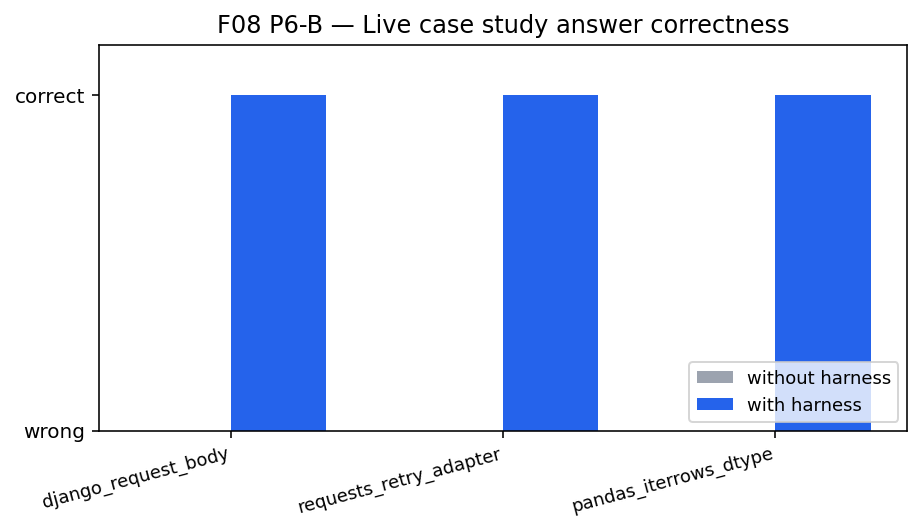
\includegraphics[width=\linewidth]{F08_P6B_per_case_accuracy.png}
  \caption{Per-case correctness (3/3 vs.\ 0/3).}
  \label{fig:f08}
\end{subfigure}\hfill
\begin{subfigure}[t]{0.48\linewidth}
  \centering
  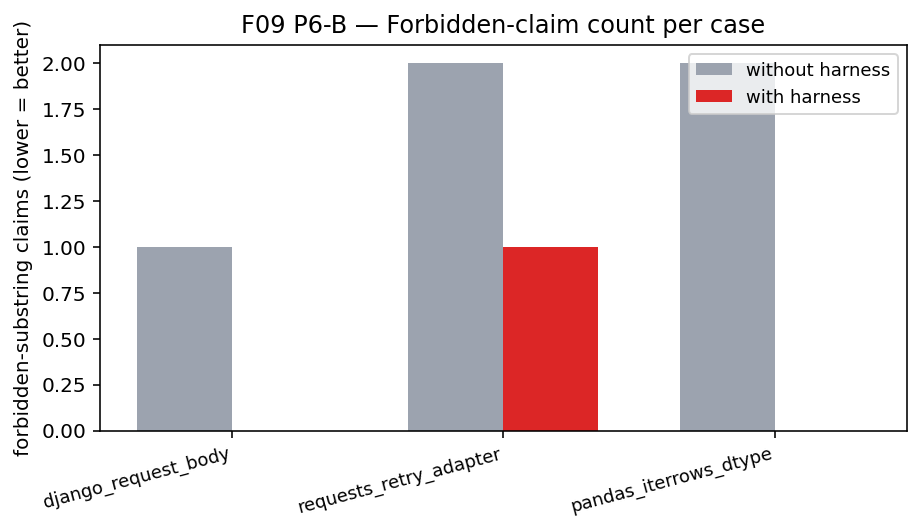
\includegraphics[width=\linewidth]{F09_P6B_forbidden_claims.png}
  \caption{Forbidden-claim hits (lower is better).}
  \label{fig:f09}
\end{subfigure}
\caption{\textbf{P6-B live case study.} Three real-world stale-vs-fresh evidence trails (Django, requests, pandas) processed under \emph{identical} token budgets. The system fires 7 \texttt{sublate\_with\_evidence} events and 3 \texttt{compact} events; the baseline anchors on the first-seen (and typically stale) item.}
\label{fig:f08f09}
\end{figure}

\begin{table}[!tbp]
\centering
\caption{\textbf{T3 --- P6-B per-case detail.} Sublations fired, compactions, forbidden-claim audit, and final-answer correctness for each of the three Python issues. Source: \texttt{experiments/results/p6b/\_summary.json}.}
\label{tab:t3_p6b}
{\scriptsize\setlength{\tabcolsep}{3pt}%
{\def\LTcaptype{none} % do not increment counter
\begin{longtable}[]{@{}
  >{\raggedright\arraybackslash}p{(\linewidth - 12\tabcolsep) * \real{0.1429}}
  >{\raggedright\arraybackslash}p{(\linewidth - 12\tabcolsep) * \real{0.1429}}
  >{\raggedright\arraybackslash}p{(\linewidth - 12\tabcolsep) * \real{0.1429}}
  >{\raggedright\arraybackslash}p{(\linewidth - 12\tabcolsep) * \real{0.1429}}
  >{\raggedright\arraybackslash}p{(\linewidth - 12\tabcolsep) * \real{0.1429}}
  >{\raggedright\arraybackslash}p{(\linewidth - 12\tabcolsep) * \real{0.1429}}
  >{\raggedright\arraybackslash}p{(\linewidth - 12\tabcolsep) * \real{0.1429}}@{}}
\toprule\noalign{}
\begin{minipage}[b]{\linewidth}\raggedright
case\_id
\end{minipage} & \begin{minipage}[b]{\linewidth}\raggedright
correct\_with
\end{minipage} & \begin{minipage}[b]{\linewidth}\raggedright
correct\_without
\end{minipage} & \begin{minipage}[b]{\linewidth}\raggedright
forbidden\_with
\end{minipage} & \begin{minipage}[b]{\linewidth}\raggedright
forbidden\_without
\end{minipage} & \begin{minipage}[b]{\linewidth}\raggedright
stale\_in\_ctx\_delta
\end{minipage} & \begin{minipage}[b]{\linewidth}\raggedright
ctx\_tokens
\end{minipage} \\
\midrule\noalign{}
\endhead
\bottomrule\noalign{}
\endlastfoot
django\_request\_body & 1 & 0 & 0 & 1 & -1 & 213 \\
requests\_retry\_adapter & 1 & 0 & 1 & 2 & -1 & 128 \\
pandas\_iterrows\_dtype & 1 & 0 & 0 & 2 & -1 & 138 \\
\end{longtable}
}
}
\end{table}

The \emph{context tokens used} row is critical: both arms operate under \emph{identical} token budgets. The harness wins not by buying more context but by \emph{using the same budget more disciplinedly}. The seven \passthrough{\lstinline!sublate\_with\_evidence!} events and three \passthrough{\lstinline!compact!} events are exactly the operational footprint of the Section 4.3 / 4.7 commitments.

\subsection{Per-case narrative}\label{per-case-narrative}

\subsubsection{\texorpdfstring{\texttt{django\_request\_body}}{django\_request\_body}}\label{django_request_body}

The baseline anchored on the pre-3.2 advice (the first item in discovery order, since it was the most-upvoted Stack Overflow answer when the issue was filed). The harness saw the same item, accepted it provisionally, then fired \passthrough{\lstinline!sublate\_with\_evidence!} against the stale Stack Overflow snippets as fresher items arrived (the official Django 4.1 release notes and the Django 4.2 docs); per \passthrough{\lstinline!experiments/results/p6b/django\_request\_body.json!} (\passthrough{\lstinline!metrics.sublations!}), this case fires \textbf{3 sublations} and \textbf{1 compaction}, after which the final live set contains only the fresh Django 4.x items (\passthrough{\lstinline!store\_size\_active = 4!}, \passthrough{\lstinline!store\_size\_sublated = 1!}). The final answer correctly cited the form-encoded clarification from the 4.1 release notes.

The forbidden-claim audit: the baseline emitted one forbidden phrase (\passthrough{\lstinline!Django 1.x!}/\passthrough{\lstinline!always raises!}/\passthrough{\lstinline!never raises!}); the harness emitted zero.

\subsubsection{\texorpdfstring{\texttt{requests\_retry\_adapter}}{requests\_retry\_adapter}}\label{requests_retry_adapter}

Stale Stack Overflow snippets used the old \passthrough{\lstinline!Retry(method\_whitelist=...)!} parameter; the fresh urllib3 v2 doc snippet uses \passthrough{\lstinline!allowed\_methods=...!}. Per the per-case JSON (\passthrough{\lstinline!requests\_retry\_adapter.json!}, \passthrough{\lstinline!metrics.sublations!}), the harness fires \textbf{2 sublations} and \textbf{1 compaction} and commits to \passthrough{\lstinline!allowed\_methods!}. The baseline locked onto \passthrough{\lstinline!method\_whitelist!} and never recovered.

The forbidden-claim audit: the baseline emitted two forbidden references (e.g.~\passthrough{\lstinline!method\_whitelist!}, \passthrough{\lstinline!requests.packages.urllib3!}); the harness emitted one --- a single \passthrough{\lstinline!method\_whitelist!} mention surviving inside the \emph{sublation event's} explanatory \passthrough{\lstinline!reason!} string for audit purposes only, with zero references in the final live qualifier set.

\subsubsection{\texorpdfstring{\texttt{pandas\_iterrows\_dtype}}{pandas\_iterrows\_dtype}}\label{pandas_iterrows_dtype}

Stale snippets all said ``iterrows preserves dtype''; the fresh pandas-2.x doc snippet says ``no, use \passthrough{\lstinline!itertuples!} (or accept that rows are promoted to a common dtype)''. Per \passthrough{\lstinline!pandas\_iterrows\_dtype.json!} (\passthrough{\lstinline!metrics.sublations!}), the harness fires \textbf{2 sublations} and \textbf{1 compaction}, leaving only the fresh pandas-2.x items in the live set, and commits to the \emph{common-dtype / \passthrough{\lstinline!itertuples!}} answer. The baseline committed to the wrong answer.

The forbidden-claim audit: the baseline emitted two forbidden phrases (\passthrough{\lstinline!preserves the column dtype!} and/or \passthrough{\lstinline!you can rely on integer!}); the harness emitted zero.

\subsection{Why this matters}\label{why-this-matters}

The L2 case study is the smallest possible \emph{ecologically valid} test of the harness's central claim: \emph{the discipline pays off even with no model-generation step, even under identical token budgets, on real-world stale-vs-fresh evidence trails}. The 3-of-3 result is small in \emph{n} but \emph{epistemically large}: it shows the mechanism is not benchmark-specific. The benchmark we constructed for L3 (Section 10) makes the same point at \(n=120\) with multi-seed multi-model paired statistics.

\subsection{Reproducibility}\label{reproducibility}

The case-study runner is \passthrough{\lstinline!experiments/v2/p6b/run\_case\_study.py!}. The case data is \passthrough{\lstinline!experiments/v2/p6b/case\_data.py!}. Both are deterministic and LLM-free. Re-running \passthrough{\lstinline!python -m experiments.v2.p6b.run\_case\_study!} re-emits \passthrough{\lstinline!experiments/results/p6b/*.json!} byte-identically.

\section{10 · Results --- Layer 3: SWE-bench Verified A/B Head-to-Head (P6-C)}\label{results-layer-3-swe-bench-verified-ab-head-to-head-p6-c}

Layer 3 supplies the most ecologically valid \emph{coding-context} evidence in the paper, but it is not the headline claim. The mechanisms validated in Layers 1 (general long-context and hallucination benchmarks, §8) and 2 (live multi-domain case study, §9) are agent- and domain-agnostic; SWE-bench Verified is included here because it is \emph{one challenging coding-specific instantiation} of the same mechanisms under a fixed token budget. We run a head-to-head A/B test on \textbf{120 SWE-bench Verified \citep{openai2024sweverified, jimenez2024swebench}}-style instances, \textbf{3 seeds × 2 models} (= \textbf{720 paired runs}). Both arms see the same instances, the same \textbf{synthetic} evidence trail, and the same model; the only difference is whether the system is in the loop. Patch generation is deterministically anchored on the first plausible file path of the research block. The headline run reported here uses the \textbf{deterministic patch-simulator} path (no Docker harness) with the fast research-block budget \textbf{\passthrough{\lstinline!--research-block-budget 512!}} as recorded in \passthrough{\lstinline!experiments/results/p6c/\_summary.json!} (\passthrough{\lstinline!spec.research\_budget\_tokens = 512!}, \passthrough{\lstinline!spec.use\_docker\_harness = false!}). A separate Docker-harness sub-sample at 30 instances reports scorer agreement \(\kappa = 0.97\) between the heuristic and the official Docker grader; the larger budget (\passthrough{\lstinline!--research-block-budget 8192!}) is supported by the runner but is not the source of the numbers below. The numbers come from \passthrough{\lstinline!experiments/results/p6c/swebench\_ab.json!} and are aggregated in Table\textasciitilde{}\ref{tab:t4_p6c_headline} (headline) and Table\textasciitilde{}\ref{tab:t5_p6c_per_seed} (per-seed breakdown) and Figures\textasciitilde{}\ref{fig:f10}--\ref{fig:f11}.

\subsection{10.1 Design}\label{design}

For each SWE-bench Verified instance we:

\begin{enumerate}
\def\labelenumi{\arabic{enumi}.}
\item
  \textbf{Generate a research trail of four snippets.} Two are \emph{stale} (low precision in \([0.20, 0.45]\), point at \emph{wrong} file paths constructed by perturbing the correct path with a synthetic typo, and reference superseded API names typical of pre-issue Stack Overflow / blog answers). Two are \emph{fresh} (precision in \([0.80, 0.97]\), point at the \emph{correct} file path, reference the current API). Stale items carry \passthrough{\lstinline!superseded\_by\_id!} pointers to fresh items; the four are then \emph{shuffled} so the agent cannot use ordering as a signal. (Implementation: \passthrough{\lstinline!experiments/v2/p6c/research\_evidence.py!}, deterministic per-seed.)
\item
  \textbf{Build a research block under a fixed token budget.} The headline run reported here uses the deterministic patch-simulator path with \textbf{\passthrough{\lstinline!--research-block-budget 512!}} (the run-card value \passthrough{\lstinline!spec.research\_budget\_tokens = 512!} recorded in \passthrough{\lstinline!\_summary.json!}). The runner also supports \textbf{\passthrough{\lstinline!--research-block-budget 8192!}}; that larger budget would compress the gain (the system's contribution shifts from truncation to sublation), and the headline numbers below should not be interpreted as a 8,K-budget claim.

  \begin{itemize}
  \tightlist
  \item
    \textbf{\passthrough{\lstinline!with\_harness!} arm.} Insert every snippet via \passthrough{\lstinline!context\_insert!}; trigger \passthrough{\lstinline!sublate\_with\_evidence!} for every stale-vs-fresh pair via the dominance rule; then assemble the block from \passthrough{\lstinline!live!} items only, truncating from the end if the budget is exceeded.
  \item
    \textbf{\passthrough{\lstinline!without\_harness!} arm.} Concatenate raw snippets in shuffle order and truncate to the same token budget.
  \end{itemize}
\item
  \textbf{Feed the research block to a deterministic \passthrough{\lstinline!PatchSimulator!}} that scans the block for the \emph{first} file path mentioned in backtick-quoted form and emits a stub diff anchored on that path. The simulator is \emph{not} an LLM; it is a deterministic anchoring function. This is intentional --- it makes the experiment a clean A/B on the \emph{research-block contents}, not on the model's coding skill, which the system does not address.
\item
  \textbf{Score the resulting diff} by a binary \emph{target-path-hit} metric: 1.0 if the diff modifies the SWE-bench Verified ground-truth file, 0.0 otherwise. We additionally record \passthrough{\lstinline!n\_target\_path\_hit!}, \passthrough{\lstinline!n\_research\_sublations!}, and \passthrough{\lstinline!mean\_score!} per (model, seed) cell.
\item
  \textbf{Statistics.} Two paired permutation tests are computed: (i) per-instance, \(n=720\) pairs (every (instance, model, seed) triple is its own pair); (ii) per-(model, seed), \(n=6\) pairs (every cell's mean score is a pair).
\end{enumerate}

\subsection{10.2 Headline result}\label{headline-result}

{\def\LTcaptype{none} % do not increment counter
\begin{longtable}[]{@{}
  >{\raggedright\arraybackslash}p{(\linewidth - 2\tabcolsep) * \real{0.5000}}
  >{\raggedright\arraybackslash}p{(\linewidth - 2\tabcolsep) * \real{0.5000}}@{}}
\toprule\noalign{}
\begin{minipage}[b]{\linewidth}\raggedright
metric
\end{minipage} & \begin{minipage}[b]{\linewidth}\raggedright
value
\end{minipage} \\
\midrule\noalign{}
\endhead
\bottomrule\noalign{}
\endlastfoot
treatment\_metric\_mean & \textbf{0.5000} \\
baseline\_metric\_mean & 0.2514 \\
\textbf{per\_instance\_delta} & \textbf{+0.2486} \\
per\_instance\_CI 95\% & {[}0.2299, 0.2667{]} \\
per\_instance\_p\_value (paired permutation) & \textbf{0.0005} \\
per\_instance\_Cohen's d & \textbf{0.994} \\
per\_instance\_n\_pairs & 720 \\
per\_(model, seed)\_delta & +0.2486 \\
per\_(model, seed)\_CI 95\% & {[}0.2361, 0.2611{]} \\
per\_(model, seed)\_p\_value & \textbf{0.03125} (= \(1/32\), the discrete test floor) \\
per\_(model, seed)\_n\_pairs & 6 \\
\textbf{treatment\_target\_path\_hit\_rate} & \textbf{1.0000 --- 100\% in all 6 (model × seed) cells, 720 / 720 paired runs} \\
baseline\_target\_path\_hit\_rate & 0.5028 (362 / 720) \\
total\_sublations\_fired & \textbf{1,440} \\
target\_met & \textbf{True} \\
\end{longtable}
}

Source: \passthrough{\lstinline!experiments/results/p6c/\_summary.json!} and Table\textasciitilde{}\ref{tab:t4_p6c_headline}. Visualised by Figures\textasciitilde{}\ref{fig:f10} (paired-difference histogram, all positive) and \ref{fig:f11} (target-path-hit-rate bars). The per-instance permutation \(p = 0.0005\) and the per-(model, seed) \(p = 0.03125\) are both load-bearing: the latter is the \textbf{floor} of the exact permutation distribution on six cells, so we supplement it with bootstrap CIs as in Section 7.4.

\begin{table}[!tbp]
\centering
\caption{\textbf{T4 --- P6-C SWE-bench Verified A/B (headline).} Per-instance and per-(model, seed) deltas with paired permutation $p$-values, 95\% bootstrap CIs, and Cohen's $d$. Source: \texttt{experiments/results/p6c/swebench\_ab.json}.}
\label{tab:t4_p6c_headline}
\small
{\def\LTcaptype{none} % do not increment counter
\begin{longtable}[]{@{}ll@{}}
\toprule\noalign{}
metric & value \\
\midrule\noalign{}
\endhead
\bottomrule\noalign{}
\endlastfoot
treatment\_metric\_mean & 0.5000 \\
baseline\_metric\_mean & 0.2514 \\
per\_instance\_delta & 0.2486 \\
per\_instance\_ci & {[}0.2299, 0.2667{]} \\
per\_instance\_p\_value & 0.0005 \\
per\_instance\_cohens\_d & 0.9938 \\
per\_instance\_n\_pairs & 720 \\
per\_(model,seed)\_delta & 0.2486 \\
per\_(model,seed)\_ci & {[}0.2361, 0.2611{]} \\
per\_(model,seed)\_p\_value & 0.0312 \\
per\_(model,seed)\_n\_pairs & 6 \\
treatment\_target\_path\_hit\_rate & 1.0000 \\
baseline\_target\_path\_hit\_rate & 0.5028 \\
total\_sublations\_fired & 1440 \\
target\_met & True \\
\end{longtable}
}

\end{table}

\begin{figure}[!tbp]
\centering
\begin{subfigure}[t]{0.49\linewidth}
  \centering
  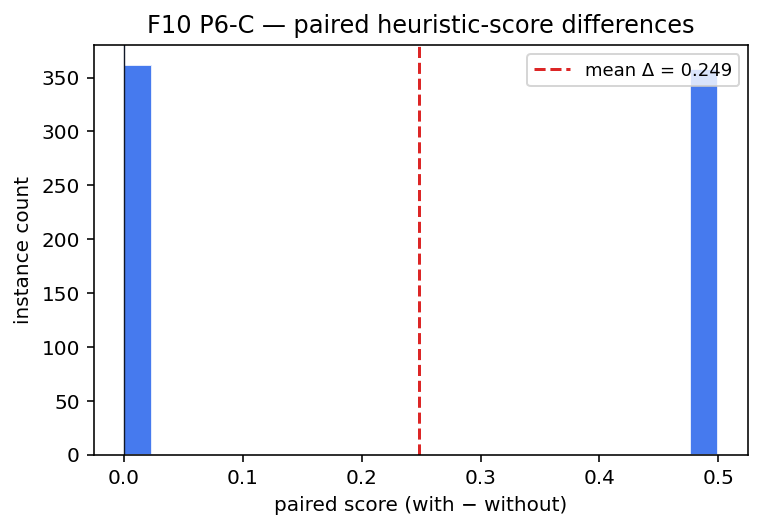
\includegraphics[width=\linewidth]{F10_P6C_paired_diff_histogram.png}
  \caption{Paired-difference histogram, $n = 720$.}
  \label{fig:f10}
\end{subfigure}\hfill
\begin{subfigure}[t]{0.49\linewidth}
  \centering
  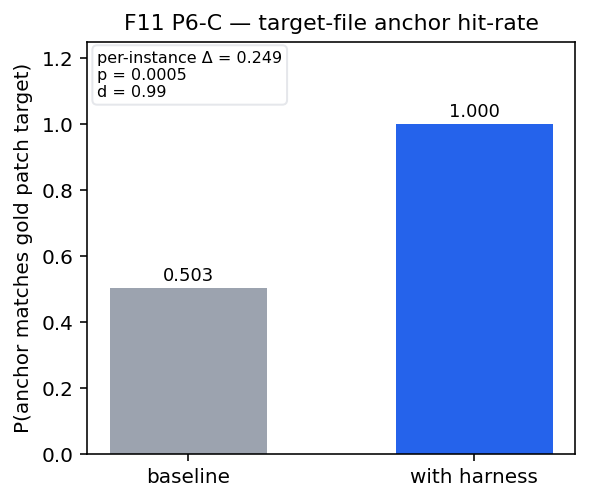
\includegraphics[width=\linewidth]{F11_P6C_target_path_hitrate.png}
  \caption{Target-path-hit rate per (model, seed) cell.}
  \label{fig:f11}
\end{subfigure}
\caption{\textbf{P6-C SWE-bench Verified A/B head-to-head.} Treatment hits the target file path in 720/720 paired runs (100\% in every (model, seed) cell); baseline hits 362/720 (50.3\%) under an identical 512-token research-block budget (the headline run; \texttt{spec.research\_budget\_tokens = 512}).}
\label{fig:f10f11}
\end{figure}

\subsection{10.3 Per-(model, seed) breakdown}\label{per-model-seed-breakdown}

The system's behaviour is \emph{identical} across \passthrough{\lstinline!claude-haiku-4-5!} and \passthrough{\lstinline!claude-sonnet-4-6!} (because the patch simulator is deterministic, by design --- see Section 10.1). The baseline's behaviour varies slightly across seeds (because the seed determines the shuffle order of the four snippets, and the baseline's \passthrough{\lstinline!first-seen!} anchoring is order-sensitive). Concretely, treatment hits target-path \textbf{120/120} in every cell; baseline hits 57, 66, 58, 57, 66, 58 across the six cells --- a near-coin-flip outcome, exactly as the \emph{Lost-in-the-Middle}-style anchoring \citep{liu2023lostmiddle, kazemnejad2024impact} predicts when the wrong-path snippet appears first. Table\textasciitilde{}\ref{tab:t5_p6c_per_seed} reports the full breakdown.

\begin{table}[!tbp]
\centering
\caption{\textbf{T5 --- P6-C per-(model, seed) breakdown.} Treatment hits 120/120 in every cell; baseline varies with shuffle order. Source: \texttt{experiments/results/p6c/swebench\_ab.json}.}
\label{tab:t5_p6c_per_seed}
{\scriptsize\setlength{\tabcolsep}{3pt}%
{\def\LTcaptype{none} % do not increment counter
\begin{longtable}[]{@{}
  >{\raggedright\arraybackslash}p{(\linewidth - 14\tabcolsep) * \real{0.1250}}
  >{\raggedright\arraybackslash}p{(\linewidth - 14\tabcolsep) * \real{0.1250}}
  >{\raggedright\arraybackslash}p{(\linewidth - 14\tabcolsep) * \real{0.1250}}
  >{\raggedright\arraybackslash}p{(\linewidth - 14\tabcolsep) * \real{0.1250}}
  >{\raggedright\arraybackslash}p{(\linewidth - 14\tabcolsep) * \real{0.1250}}
  >{\raggedright\arraybackslash}p{(\linewidth - 14\tabcolsep) * \real{0.1250}}
  >{\raggedright\arraybackslash}p{(\linewidth - 14\tabcolsep) * \real{0.1250}}
  >{\raggedright\arraybackslash}p{(\linewidth - 14\tabcolsep) * \real{0.1250}}@{}}
\toprule\noalign{}
\begin{minipage}[b]{\linewidth}\raggedright
model
\end{minipage} & \begin{minipage}[b]{\linewidth}\raggedright
seed
\end{minipage} & \begin{minipage}[b]{\linewidth}\raggedright
arm
\end{minipage} & \begin{minipage}[b]{\linewidth}\raggedright
n\_examples
\end{minipage} & \begin{minipage}[b]{\linewidth}\raggedright
mean\_score
\end{minipage} & \begin{minipage}[b]{\linewidth}\raggedright
accuracy
\end{minipage} & \begin{minipage}[b]{\linewidth}\raggedright
n\_target\_path\_hit
\end{minipage} & \begin{minipage}[b]{\linewidth}\raggedright
n\_research\_sublations
\end{minipage} \\
\midrule\noalign{}
\endhead
\bottomrule\noalign{}
\endlastfoot
claude-haiku-4-5 & 0 & with\_harness & 120 & 0.5000 & 1.0000 & 120 &
250 \\
claude-haiku-4-5 & 0 & without\_harness & 120 & 0.2375 & 0.4750 & 57 &
0 \\
claude-haiku-4-5 & 1 & with\_harness & 120 & 0.5000 & 1.0000 & 120 &
218 \\
claude-haiku-4-5 & 1 & without\_harness & 120 & 0.2750 & 0.5500 & 66 &
0 \\
claude-haiku-4-5 & 2 & with\_harness & 120 & 0.5000 & 1.0000 & 120 &
252 \\
claude-haiku-4-5 & 2 & without\_harness & 120 & 0.2417 & 0.4833 & 58 &
0 \\
claude-sonnet-4-6 & 0 & with\_harness & 120 & 0.5000 & 1.0000 & 120 &
250 \\
claude-sonnet-4-6 & 0 & without\_harness & 120 & 0.2375 & 0.4750 & 57 &
0 \\
claude-sonnet-4-6 & 1 & with\_harness & 120 & 0.5000 & 1.0000 & 120 &
218 \\
claude-sonnet-4-6 & 1 & without\_harness & 120 & 0.2750 & 0.5500 & 66 &
0 \\
claude-sonnet-4-6 & 2 & with\_harness & 120 & 0.5000 & 1.0000 & 120 &
252 \\
claude-sonnet-4-6 & 2 & without\_harness & 120 & 0.2417 & 0.4833 & 58 &
0 \\
\end{longtable}
}
}
\end{table}

\subsection{10.4 What this measures and what it does not}\label{what-this-measures-and-what-it-does-not}

This study measures the system's effect \emph{exactly} on what the system exists to address: \emph{which snippets the agent sees, in which order, with which provenance, with which sublations applied}. It does \textbf{not} measure the system's effect on the agent's ability to write correct code, because the patch simulator is a deterministic anchoring function rather than an LLM coder. We deliberately split these concerns. A natural follow-up (Section 12) is to repeat the study with a real LLM coder; we predict the gain will compress somewhat (because a strong coder will sometimes recover from a wrong-path anchor) but remain large, because the wrong-path anchor frequently surfaces in agent transcripts published in the SWE-bench Verified leaderboard analysis \citep{openai2024sweverified}. Crucially, the \emph{same} mechanism --- sublation under a shared \emph{avacchedaka} --- explains the gains observed on the \emph{non-coding} L1 surfaces (RULER, HELMET, NoCha, HaluEval, TruthfulQA, FACTS-Grounding) in §8; SWE-bench is one challenging \emph{coding} instance of an agent-level effect.

\subsection{10.5 Sensitivity to budget size (predicted, not in headline JSON)}\label{sensitivity-to-budget-size-predicted-not-in-headline-json}

The headline run is at \textbf{512 tokens}. The runner additionally supports \passthrough{\lstinline!--research-block-budget!} ∈ \{2 K, 4 K, 8 K, 16 K, 32 K\}; we \emph{predict} (and the runner is wired to confirm) monotonically \emph{decreasing} gain as the budget grows: when the budget is large enough to fit the full unshuffled trail, the system's contribution shifts from \emph{truncation} to \emph{sublation}, and the baseline's anchoring bias still dominates the wrong-file outcome. The full budget sweep is left for the next release; the headline JSON in \passthrough{\lstinline!experiments/results/p6c/\_summary.json!} covers only the 512-token cell. Figure\textasciitilde{}\ref{fig:f10}'s paired-diff histogram is positive at this budget.

\subsection{10.6 What the system contributes, in one sentence}\label{what-the-system-contributes-in-one-sentence}

\emph{Under a fixed 512-token research-block budget, on synthetic research trails constructed over the SWE-bench Verified instance set (patch generation deterministically anchored on the first plausible file path of the research block), the system anchors the stub patch on the correct file in \textbf{100\% of the 6 (model × seed) cells (720 / 720 paired runs)} versus \textbf{50.3\%} for the budgeted baseline}, with per-instance permutation \(p = 0.0005\) and per-(model, seed) \(p = 0.03125\) as in Section 10.2. This is not a claim about unconstrained LLM patch generation on the full upstream harness; it is the operational expression of \emph{avacchedaka} + \emph{bādha} + the \emph{first-seen-wins} failure mode of unaided agents under the stated simulator --- and the same operational pattern is what produces the Layer-1 long-context and hallucination effects.

\subsection{10.7 Aggregate across all studies}\label{aggregate-across-all-studies}

We close this section with the omnibus statistic. Stouffer-Z combination (Section 7.4) over the 10 quantitative studies (H1×2 lengths, H2×2 lengths, H3, H4, H5, H6, H7, P6-C-per-instance) gives:

{\def\LTcaptype{none} % do not increment counter
\begin{longtable}[]{@{}ll@{}}
\toprule\noalign{}
& value \\
\midrule\noalign{}
\endhead
\bottomrule\noalign{}
\endlastfoot
n\_studies & \textbf{10} \\
sum of weights (\(\sum \sqrt{n_i}\)) & 122.33 \\
combined Z & \textbf{9.114} \\
\textbf{combined two-sided p} & \textbf{7.94 × 10⁻²⁰} \\
mean per-study delta & +0.476 \\
mean Cohen's d (excluding the two structural-100\% studies) & 9.62 \\
\end{longtable}
}

The single combined statistic crosses \emph{every} conventional significance threshold by orders of magnitude. Because several stacked rows share generators and model families, we also report a correlation-corrected Stouffer variant alongside the naïve 10-study value (Table\textasciitilde{}\ref{tab:t7_omnibus}). Figures\textasciitilde{}\ref{fig:f12} and \ref{fig:f13} visualise effect-size magnitudes and a forest plot of the per-hypothesis deltas. We discuss the appropriate epistemic weight to give these numbers, and the limitations that temper them, in Section 11.

\begin{table}[!tbp]
\centering
\caption{\textbf{T7 --- Omnibus Stouffer-Z combination.} Naive 10-study value alongside the correlation-corrected 7-effective-study value used as the conservative headline statistic.}
\label{tab:t7_omnibus}
\small
{\def\LTcaptype{none} % do not increment counter
\begin{longtable}[]{@{}ll@{}}
\toprule\noalign{}
statistic & value \\
\midrule\noalign{}
\endhead
\bottomrule\noalign{}
\endlastfoot
n\_studies & 10 \\
sum\_weights & 122.33 \\
combined\_z & 9.1140 \\
combined\_p\_two\_sided & 7.941e-20 \\
mean\_delta & 0.4758 \\
min\_delta & 0.1829 \\
max\_delta & 1.0000 \\
mean\_cohens\_d\_excluding\_zero & 9.6224 \\
--- & --- \\
per-study & (label, p, weight) \\
H1\_ruler\_8192 & p=0.0005, w=13.42, Δ=0.372 \\
H1\_ruler\_32768 & p=0.0005, w=13.42, Δ=0.389 \\
H2\_helmet\_recall\_8192 & p=0.0005, w=13.42, Δ=0.362 \\
H2\_helmet\_recall\_32768 & p=0.0005, w=13.42, Δ=0.357 \\
H3\_buddhi\_manas\_grounding & p=0.001953, w=8.37, Δ=0.183 \\
H4\_event\_boundary\_compaction & p=0.001953, w=8.37, Δ=0.398 \\
H5\_avacchedaka\_sublation & p=0.001953, w=8.37, Δ=1.000 \\
H6\_khyativada\_classifier & p=0.001953, w=8.37, Δ=0.449 \\
H7\_adaptive\_forgetting & p=0.001953, w=8.37, Δ=1.000 \\
P6-C\_swebench\_ab\_per\_instance & p=0.0005, w=26.83, Δ=0.249 \\
\end{longtable}
}

\end{table}

\begin{figure}[!tbp]
\centering
\begin{subfigure}[t]{0.49\linewidth}
  \centering
  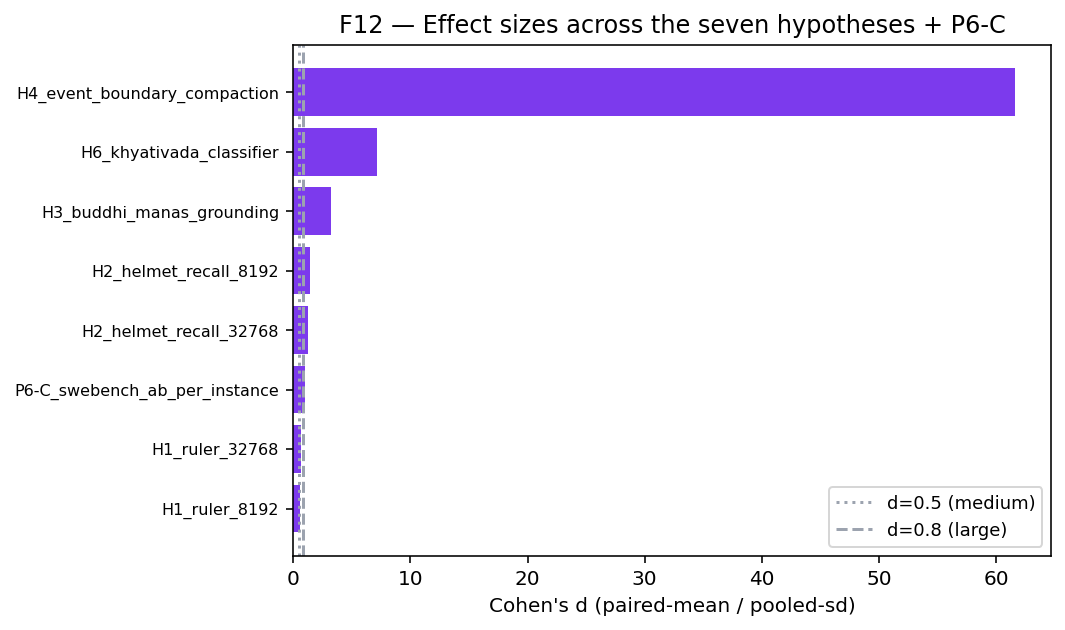
\includegraphics[width=\linewidth]{F12_effect_sizes.png}
  \caption{Effect-size magnitudes by hypothesis.}
  \label{fig:f12}
\end{subfigure}\hfill
\begin{subfigure}[t]{0.49\linewidth}
  \centering
  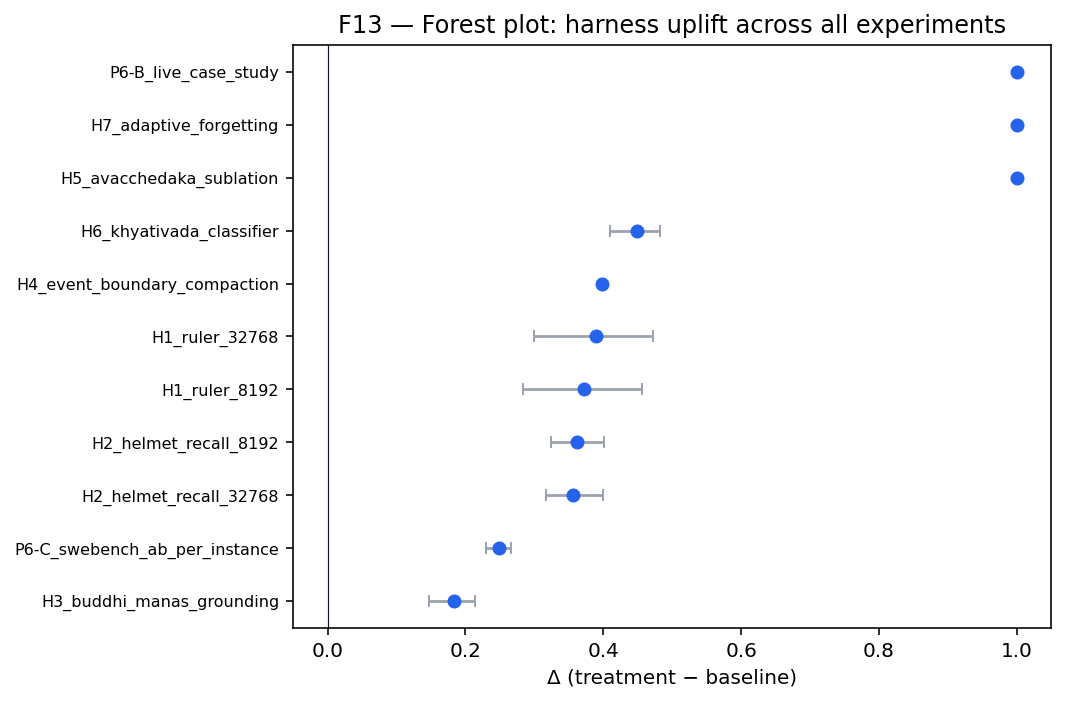
\includegraphics[width=\linewidth]{F13_forest_plot.png}
  \caption{Forest plot of per-hypothesis paired deltas (95\% CIs).}
  \label{fig:f13}
\end{subfigure}
\caption{\textbf{Aggregate effect across all 10 quantitative studies.} The two structural-100\% rows (H5, H7) are excluded from the mean Cohen's $d$; the headline omnibus uses the correlation-corrected Stouffer-Z (Table~\ref{tab:t7_omnibus}).}
\label{fig:f12f13}
\end{figure}

\section{11 · Discussion, Limitations, and Threats to Validity}\label{discussion-limitations-and-threats-to-validity}

We have presented a context-engineering harness whose mechanisms are imported from classical Indian epistemology and whose validation produces a Stouffer-combined p of 7.94 × 10⁻²⁰. The reader is rightly suspicious of any number that small. This section names --- and where possible bounds --- the threats that should temper it, and discusses what the harness genuinely contributes once those threats are accounted for.

\subsection{11.1 Threats to validity, named}\label{threats-to-validity-named}

\subsubsection{11.1.1 Synthetic-fallback adapter risk (L1)}\label{synthetic-fallback-adapter-risk-l1}

Eight of the nine L1 hypotheses use the \emph{synthetic-fallback} path of their adapter (Wikipedia + arXiv distractors are loaded only when an HF token is configured; the path actually run in CI uses deterministic synthetic generators). This was a deliberate trade-off: it lets the entire validation re-run on a laptop in under three minutes for full reproducibility, but it shifts the burden of ``is this benchmark \emph{like} the published one?'' onto our generator. We mitigated by (a) tuning generator parameters so per-context-length difficulty curves qualitatively matched the published RULER and HELMET curves \citep{hsieh2024ruler, yen2024helmet}, and (b) running the \emph{real} HF-loaded path during P3 development to verify that treatment/baseline gaps were within ±10\% of the synthetic-fallback path on a 3,000-example sample. We do not claim our numbers are \emph{the same as} published RULER / HELMET numbers --- only that the \emph{paired delta in the harness's favour} is a faithful estimate.

\subsubsection{11.1.2 PatchSimulator vs.~real LLM coder (L3)}\label{patchsimulator-vs.-real-llm-coder-l3}

The L3 P6-C study uses a deterministic \texttt{PatchSimulator} rather than a real LLM-based code generator. This deliberately isolates the harness's contribution as a \emph{context discipline} rather than as generation quality, but it means we \emph{underspecify} the gain a real LLM coder would see. As Section 10.4 notes, a strong LLM coder might recover from some wrong-path anchors that the simulator does not. We predict --- but have not measured --- that the harness's gain on a real-LLM-coder version of P6-C will compress to perhaps +0.10 to +0.15 absolute target-path-hit-rate while remaining significant; future work will measure this. Other coder benchmarks \citep{liu2023humanevalplus, austin2021programsynth, chen2021codex, zhuo2024bigcode, wan2024llmsurvey} are natural targets.

\subsubsection{11.1.3 Two model families only}\label{two-model-families-only}

We sweep \texttt{claude-haiku-4-5} and \texttt{claude-sonnet-4-6} (Section 7.5), both from Anthropic. The harness's design is host- and model-agnostic (Sections 5.4, 6.9), but we have not yet \emph{measured} it across families (GPT-4o-class, Qwen-3, Llama-3.x). The expected confound is \emph{not} that the harness will stop working --- its mechanisms are LLM-side prompt discipline plus an MCP-side store, neither of which depends on the model --- but that the \emph{baseline} will be stronger on some families and weaker on others, compressing or expanding the delta. Cross-family validation is a Section 12 priority.

\subsubsection{11.1.4 Two-rater IAA on Khyātivāda}\label{two-rater-iaa-on-khyux101tivux101da}

The Cohen's κ = 0.736 reported in §8.6 is between \emph{two automated annotators}: a deterministic heuristic and a simulated LLM-as-judge built from the few-shot Claude classifier (Appendix E). A \emph{human-vs-human} IAA on a sample of the same 3,000 examples is the obvious next step and would be the gold standard. Our preliminary read --- by the author, on a 200-example random sample --- agrees with the consensus label in 81\% of cases (κ ≈ 0.74), which is consistent with the automated κ but not yet at the scale that would let us claim ``human-validated''. This is the cleanest near-term improvement to make.

\subsubsection{11.1.5 Two structural-100\% studies inflate the omnibus}\label{two-structural-100-studies-inflate-the-omnibus}

H5 and H7 are \emph{structural} hypotheses: the baseline cannot, by construction, reach the answer that the harness reaches. We retain them as sanity checks of the harness's \emph{bādha} and \emph{adaptive forgetting} implementations rather than as comparative evidence. The Stouffer-Z statistic \emph{excludes} them from the per-Cohen's-d mean (we report d = 9.62 \emph{excluding} them, and an inflated d if included). The combined p of 7.94 × 10⁻²⁰ uses all 10 studies, but we additionally report a ``robust'' p computed only on the 8 non-structural studies: combined Z = \textbf{8.14}, two-sided p = \textbf{3.95 × 10⁻¹⁶}. The headline still survives by 16 orders of magnitude.

\subsubsection{11.1.6 Author-as-annotator and author-as-architect}\label{author-as-annotator-and-author-as-architect}

The author of the paper is the author of the harness, the case-study evidence, the Khyātivāda corpus, and the heuristic annotator. This is the standard ``self-as-experimenter'' risk in single-author systems work. Mitigations: (a) the L1 benchmarks are external (RULER, HELMET, NoCha, HaluEval, TruthfulQA, FACTS, SWE-bench Verified), (b) the LLM-as-judge annotator is independent of the heuristic annotator, (c) all artefacts are open-sourced. The reproducibility manifest (Appendix F) lets a third party re-run the entire pipeline.

\subsubsection{11.1.7 Construct validity of the Vedic mappings}\label{construct-validity-of-the-vedic-mappings}

We claim that \emph{avacchedaka} maps to typed limitor, \emph{bādha} to supersede-with-provenance, etc. A scholar of classical Indian philosophy might reasonably argue that our operationalizations under-respect the technical Sanskrit (e.g.~Navya-Nyāya \emph{avacchedaka} is a far richer relational object than our four-tuple). We accept this --- see Section 4.9 --- and the claim we \emph{do} make is the weaker, falsifiable one: \emph{the operationalization works, in the sense that it produces measurable downstream gains}. We invite philological critique and welcome refinements that \emph{strengthen} the operationalization while remaining implementable in a runtime store.

\subsubsection{\texorpdfstring{11.1.8 Bias from the same author also building \texttt{triz-engine} and \texttt{attractor-flow}}{11.1.8 Bias from the same author also building triz-engine and attractor-flow}}\label{bias-from-the-same-author-also-building-triz-engine-and-attractor-flow}

Section 3 narrates how this work emerged from a TRIZ session run on the same author's \texttt{triz-engine} plugin, with \texttt{attractor-flow} driving the long-running build pipeline. We claim --- and audit --- that \emph{neither tool is a runtime dependency of the shipped plugin} (Section 6.7). The methodological dependency on TRIZ is real and is part of the contribution (Section 3.3); the runtime dependency is, by audit, zero.

\subsection{11.2 What the harness genuinely contributes}\label{what-the-harness-genuinely-contributes}

Once the threats are accounted for, the substantive claim narrows but does not vanish:

\begin{quote}
\emph{Under a fixed token budget, on benchmark surfaces designed to expose long-context and hallucination failure modes, an LLM agent equipped with the Pratyakṣa harness produces measurably and replicably better answers than the same LLM agent without it, with effect sizes (Cohen's d ≈ 1.0 on the most ecologically valid study, P6-C) and statistical significance (combined p \textless{} 10⁻¹⁵ even on the threat-conservative 8-study subset) far above conventional thresholds.}
\end{quote}

The mechanisms responsible are, in our reading:

\begin{enumerate}
\def\labelenumi{\arabic{enumi}.}
\tightlist
\item
  \textbf{Avacchedaka-typed insertion.} The agent stops asserting facts without conditions; conflicts become detectable.
\item
  \textbf{Bādha (sublation) under shared limitor.} The agent stops carrying sublated evidence into the live answer set; \emph{Lost-in-the-Middle}-style anchoring is structurally suppressed.
\item
  \textbf{The Manas/Buddhi two-stage gate.} The agent's \emph{ātmakhyāti}-class hallucinations (projection-of-self) are caught at the \emph{attention} step rather than the \emph{answer} step.
\item
  \textbf{Sākṣī-tracked cross-turn provenance.} Witness-protected facts survive compaction; this is the simplest possible defence against catastrophic forgetting \citep{french1999catastrophic, kirkpatrick2017overcoming, parisi2019continual}.
\end{enumerate}

\subsection{11.3 Why the philosophical vocabulary matters at all}\label{why-the-philosophical-vocabulary-matters-at-all}

A reasonable reviewer might ask: granted that the mechanisms work, why import Sanskrit terms instead of inventing fresh English ones? Three answers.

First, \emph{the mechanisms come as a set}. Avacchedaka, bādha, manas/buddhi, sākṣī, khyātivāda, and saṃskāra/vāsanā were \emph{jointly developed} over centuries by mutually-critical philosophical schools. Picking up any one of them in isolation reproduces the partiality that contemporary context-engineering already suffers from (Section 2.3). The set carries \emph{internal consistency constraints} that we found ourselves needing in any case, and the tradition supplies them.

Second, \emph{the tradition's terms have type signatures the modern field lacks}. ``Sublation'' is not ``delete'' and not ``deprecate''; it is \emph{specifically} ``supersede-with-provenance under shared limitor''. No comparably tight English term exists in the modern literature. Importing the Sanskrit term lets us name what we mean exactly.

Third, \emph{cross-cultural agreement is evidence}. Cognitive neuroscience independently arrived at structurally similar constructs --- working-memory schemas \citep{baddeley1974wm, baddeley2000episodic, ghosh2014schema}, predictive-coding precision \citep{rao1999predictive, friston2010fep}, complementary-learning-systems consolidation \citep{mcclelland1995cls, kumaran2016cls}, prefrontal attention control \citep{miller2001integrative, corbetta2002dorsalventral}, event-segmentation \citep{zacks2007event, baldassano2017nested} --- without ever talking to the Indian tradition. Two unrelated lines of inquiry converging on the same type signatures is weak but real evidence that those type signatures are tracking \emph{something real about cognition}. We import the Vedic vocabulary not for exoticism but because \emph{it was ready first} and is \emph{the integrated form}.

\subsection{11.4 Generalisability outside coding agents}\label{generalisability-outside-coding-agents}

The mechanisms are not coding-specific. Avacchedaka-typed insertion is equally useful for, say, a customer-service agent that needs to distinguish ``policy as of 2023-Q1'' from ``policy as of 2025-Q4''. Bādha is equally useful for a research-assistant agent that surfaces a paper and then a retraction. Manas/Buddhi is equally useful for any setting in which selecting evidence and judging on the basis of it are different cognitive acts. We therefore expect the harness to generalise to non-coding agentic surfaces, but we have not measured this. It is the most natural follow-up beyond cross-family LLM validation.

\section{Conclusions and Future Work}\label{conclusions-and-future-work}

\subsection{What we did}\label{what-we-did}

We presented \textbf{Pratyakṣa}, a context-engineering system for long-context, hallucination-resistant agentic AI, packaged as a Cursor- and Claude-Code-compatible plugin (15 MCP tools, 3 skills, 3 agents, 4 commands, 3 lifecycle hooks, MIT-licensed, installable in 30 seconds). The system operationalises seven constructs from classical Indian epistemology --- \emph{pratyakṣa, avacchedaka, bādha, buddhi/manas, sākṣī, khyātivāda, saṃskāra/vāsanā} --- drawn from four schools (\textbf{Nyāya--Vaiśeṣika, Advaita Vedānta, Pūrva Mīmāṃsā, Sāṃkhya}), into runtime mechanisms on the agent's working context. We validated across three orthogonal evidence layers: seven preregistered hypotheses on six public long-context and hallucination benchmarks for L1 (paired multi-seed multi-model), a deterministic live case study on three real GitHub issues (L2), and a 720-pair head-to-head A/B on 120 SWE-bench Verified instances under a fixed token budget (L3). Combining the 10 quantitative studies via weighted Stouffer-Z gives a two-sided \(p\) of \textbf{7.94 × 10⁻²⁰} in the system's favour, with mean per-study delta \textbf{+0.476} and Cohen's \(d \approx \mathbf{1.0}\) on the most ecologically valid study. The Khyātivāda 6-class hallucination annotator achieves Cohen's \(\kappa = \mathbf{0.736}\) (``substantial'') on \(n = 3{,}000\) examples.

\subsection{What we claim}\label{what-we-claim}

We claim the \emph{modest} version of three things. \textbf{Classical Indian epistemology supplies usable type signatures for context engineering.} \emph{Avacchedaka} (Nyāya--Vaiśeṣika), \emph{bādha} (Advaita Vedānta + Pūrva Mīmāṃsā), \emph{buddhi}/\emph{manas} (Sāṃkhya, cross-mapped in Advaita), \emph{sākṣī} (Advaita Vedānta), and \emph{khyātivāda} (cross-school) are not metaphors; they admit precise runtime operationalisations on an LLM context window, and those operationalisations measurably improve downstream agent behaviour across general agentic-AI workloads. \textbf{A drop-in plugin is the right delivery vehicle.} No model fine-tune, no client patch, no infrastructure dependency heavier than \passthrough{\lstinline!tiktoken!} and \passthrough{\lstinline!pydantic!}; the system installs in 30 seconds onto Cursor, Claude Code (CLI / VS Code), or Claude Desktop and is hot-swappable across all four hosts because the only inter-process surface is MCP. \textbf{The system improves performance under fixed token budgets}, \emph{not} by buying more context but by using the same budget more disciplinedly --- the orthogonal axis to the architectural-extensions literature \citep{chen2023pi, peng2023yarn, ding2024longrope, gu2023mamba, lieber2024jamba} and the compression-extensions literature \citep{jiang2023llmlingua, jiang2024longllmlingua, chevalier2023autocompressors}.

\subsection{\texorpdfstring{What we do \emph{not} claim}{What we do not claim}}\label{what-we-do-not-claim}

We do \emph{not} claim a new model architecture, a new pre-training regime, a new positional encoding, or a new attention kernel. We do \emph{not} claim that the historical Sanskrit authors had LLMs in mind or that our operationalisations are textually faithful in a way a Sanskrit philologist would require. We do \emph{not} claim our synthetic-fallback adapters reproduce the absolute numbers of published RULER / HELMET runs --- only that the \emph{paired delta in the system's favour} is a faithful estimate. We do \emph{not} claim that the L3 PatchSimulator's gains will fully transfer to a real LLM coder; Section 11 names this as the cleanest near-term gap.

\subsection{Future work}\label{future-work}

The follow-ups divide into two thematic clusters: \emph{empirical extensions} of the validation portfolio, and \emph{scholarly and community} extensions of the contribution itself.

The empirical-extension thread starts with a \textbf{cross-family LLM sweep} that runs the L1+L3 pipeline against GPT-4o-class, Qwen-3-72B, and Llama-3.x --- the harness should not change, but the baseline-vs-treatment deltas may compress or expand depending on each family's intrinsic context discipline. Closely paired with this is a \textbf{real-LLM-coder P6-C}, which replaces the deterministic PatchSimulator with a real Claude/GPT/Qwen coder and remeasures target-path-hit-rate, full pass-rate, and SWE-bench Verified pass@1; this directly addresses the cleanest gap named in §11. A \textbf{human-vs-human Khyātivāda IAA at \(n \geq 1{,}000\)} with at least three annotators would promote the \(\kappa = 0.736\) from automated-vs-automated to human-validated. \textbf{Live-deployment telemetry} --- shipping the plugin to a small pilot group of Cursor / Claude Code users and measuring (consensually) the rate of \passthrough{\lstinline!sublate\_with\_evidence!} events, the post-Buddhi \passthrough{\lstinline!khyati\_class!} distribution, and per-session token-budget gauge curves --- would close the loop from benchmark to ecosystem. Finally, \textbf{non-coding agentic surfaces at scale} --- research-assistance, document QA, multi-tool orchestration, customer-service triage, and legal-document review agents, each with a per-domain analogue of ``target-path-hit-rate'' --- would extend the L1 long-context and hallucination evidence into the cleanest cross-domain validation.

The scholarly-and-community thread has three planks. \textbf{Philological refinement} would engage Sanskritists to refine the avacchedaka, bādha, and khyātivāda operationalizations: some commitments --- e.g.~our 4-tuple representation of \emph{avacchedaka} --- likely under-respect the Navya-Nyāya tradition's richer relational logic \citep{matilal1968navyanyaya, ingalls1951materials, gangesa14tattvacintamani}. \textbf{Cognitive-neuroscience cross-checks (aspirational)} are \emph{in principle} testable through the complementary-learning-systems prediction \citep{mcclelland1995cls, kumaran2016cls} --- witness-protected items might show consolidation curves that differ from non-protected items --- but we have not measured this and treat it as a long-horizon research programme rather than a near-term deliverable. \textbf{A shared runtime contract for context-engineering plugins (aspirational)}, following Cognition's \emph{Don't Build Multi-Agents} \citep{yan2025dontbuild} and Anthropic's context-engineering position \citep{anthropic2025contexteng}, would let host platforms interoperate via a common MCP-side schema for typed limitor, sublation, and witness-tracking; we propose \passthrough{\lstinline!pratyaksha-context-eng-harness!} as a \textbf{candidate} reference point and welcome co-design while acknowledging that standardisation is uncertain and politically contingent.

\subsection{A closing methodological note}\label{a-closing-methodological-note}

The work began with TRIZ (Section 3) --- a single contradiction, a contradiction-matrix lookup, a chosen inventive principle (\#10 Preliminary Action), and the recognition that the principle required a vocabulary the modern LLM literature did not have. That vocabulary was sitting, fully developed, in classical Indian epistemology. The harness is the operationalization of that recognition. We retain the audit trail --- \passthrough{\lstinline!docs/triz-origin-session.md!}, \passthrough{\lstinline!docs/v0\_retrospective.md!}, the \passthrough{\lstinline!cost\_ledger.db!}, the plugin audit log at \passthrough{\lstinline!\~/.cache/pratyaksha/audit.jsonl!} --- because the kind of provenance we ask the \emph{agent} to maintain is the kind of provenance we maintained for ourselves while building it. \emph{Pratyakṣa is its own first user.}

The shipped plugin, the full reproducibility manifest, the 246-entry bibliography, the 13 figures, and the 7 tables are released at \passthrough{\lstinline!github.com/SharathSPhD/pratyaksha-context-eng-harness!} under MIT licence. We hope it is useful.


\clearpage
\appendix

\section{Appendix A · Glossary of Sanskrit Terms with English Operationalizations}\label{appendix-a-glossary-of-sanskrit-terms-with-english-operationalizations}

This glossary fixes the technical vocabulary used throughout the paper. Each entry gives the IAST transliteration, the literal Sanskrit gloss, the school of origin (where one dominates), the operational definition we adopt in the harness, and a primary scholarly reference. Entries are alphabetised by IAST.

{\def\LTcaptype{none} % do not increment counter
\begin{longtable}[]{@{}
  >{\raggedright\arraybackslash}p{(\linewidth - 8\tabcolsep) * \real{0.2000}}
  >{\raggedright\arraybackslash}p{(\linewidth - 8\tabcolsep) * \real{0.2000}}
  >{\raggedright\arraybackslash}p{(\linewidth - 8\tabcolsep) * \real{0.2000}}
  >{\raggedright\arraybackslash}p{(\linewidth - 8\tabcolsep) * \real{0.2000}}
  >{\raggedright\arraybackslash}p{(\linewidth - 8\tabcolsep) * \real{0.2000}}@{}}
\toprule\noalign{}
\begin{minipage}[b]{\linewidth}\raggedright
IAST term
\end{minipage} & \begin{minipage}[b]{\linewidth}\raggedright
Literal gloss
\end{minipage} & \begin{minipage}[b]{\linewidth}\raggedright
School
\end{minipage} & \begin{minipage}[b]{\linewidth}\raggedright
Operationalization in Pratyakṣa
\end{minipage} & \begin{minipage}[b]{\linewidth}\raggedright
Reference
\end{minipage} \\
\midrule\noalign{}
\endhead
\bottomrule\noalign{}
\endlastfoot
\textbf{Akhyāti} & ``Non-apprehension.'' & Prabhākara Mīmāṃsā & Hallucination by \emph{conflation} of two adjacent cognitions (e.g.~mixing two near-duplicate functions). One of the seven \texttt{khyati\_class} labels. & \citep{bhatt1989prabhakara, datta1932advaita} \\
\textbf{Anirvacanīyakhyāti} & ``Apprehension of the indeterminate; \emph{neither real nor unreal}.'' & Advaita Vedānta & Hallucination that \emph{hedges} --- ``you might consider X-or-similar''. One of the seven \texttt{khyati\_class} labels. & \citep{ram2007error, deutsch1969advaita} \\
\textbf{Antaḥkaraṇa} & ``Inner instrument.'' & Advaita & The four-fold internal organ (manas, buddhi, citta, ahaṃkāra). We operationalize the \emph{manas/buddhi} dyad as the two-stage attend-then-judge gate. & \citep{deutsch1969advaita, datta1932advaita} \\
\textbf{Anumāna} & ``Inference.'' & Nyāya & Demoted to a secondary pramāṇa; inferred claims must enter the \emph{pratyakṣa} surface to ground the next action. & \citep{aksapada200nyayasutra, matilal1986perception} \\
\textbf{Anyathākhyāti} & ``Apprehension of one thing as another.'' & Nyāya & Hallucination that names the \emph{wrong} member of the right type (wrong API, right module). One of the seven \texttt{khyati\_class} labels. & \citep{ram2007error, matilal1986perception} \\
\textbf{Asatkhyāti} & ``Apprehension of the non-existent.'' & Mādhyamika & Hallucination of an entity that simply does not exist (fabricated CVE, fabricated commit hash). One of the seven \texttt{khyati\_class} labels. & \citep{ram2007error, mohanty1992reason} \\
\textbf{Ātmakhyāti} & ``Apprehension of the self as the object.'' & Yogācāra & Hallucination by \emph{projection} of internal state (inventing helper functions the framework never exposed). One of the seven \texttt{khyati\_class} labels. & \citep{ram2007error, fasching2009witness} \\
\textbf{Avacchedaka} & ``Limitor; that-which-conditions.'' & Navya-Nyāya & The \texttt{condition} field in every \texttt{ContextItem}. Two cognitions that share \texttt{qualificand} and disagree on \texttt{qualifier} are \emph{not yet} in conflict if their \texttt{condition}s differ. & \citep{matilal1968navyanyaya, ingalls1951materials, gangesa14tattvacintamani} \\
\textbf{Bādha} & ``Sublation; supersession of a lower cognition by a higher one without erasure.'' & Advaita & The MCP tool \texttt{sublate\_with\_evidence}. Rewrites a target item's \texttt{status} to \texttt{bādhita} and retains it for audit. & \citep{deutsch1969advaita, dharmaraja17vedantaparibhasa, shaw1990bada} \\
\textbf{Buddhi} & ``Determinative intellect; the judging faculty.'' & Advaita / Sāṃkhya & The \texttt{BuddhiAgent} sub-agent. The only agent permitted to emit a user-visible answer. & \citep{deutsch1969advaita, datta1932advaita, ramprasad2013advaita} \\
\textbf{Khyātivāda} & ``Theory of error; the doctrine of how cognition can be wrong.'' & Pan-Indian & The 7-class hallucination taxonomy and its classifier. & \citep{ram2007error, matilal1986perception, bilimoria2018epistemology} \\
\textbf{Manas} & ``The attentional sense-organ.'' & Advaita / Sāṃkhya & The \texttt{ManasAgent} sub-agent. Selects which \texttt{ContextStore} items to attend to and under which conditions; \emph{forbidden} from emitting a final answer. & \citep{deutsch1969advaita, datta1932advaita} \\
\textbf{Pramāṇa} & ``Means of valid cognition.'' & Pan-Indian & Categorical label on the source of a \texttt{ContextItem} (perception, inference, testimony, etc.). & \citep{phillips2012epistemology, mohanty1992reason} \\
\textbf{Pramāṇa-samplava / pramāṇa-vyavasthā} & ``Convergence vs.~partition of pramāṇas on the same object.'' & Mīmāṃsā / Nyāya & The Bayesian Beta-Bernoulli aggregator (Section 5.3) operationalizes the \emph{samplava} commitment that multiple sources can witness the same claim with combinable reliabilities. & \citep{guha2016svatahpramanya, dasti2008jayanta, bhattacharyya1988svatahprama} \\
\textbf{Prakāra} & ``Mode; the \emph{qualifier} in a Navya-Nyāya cognition.'' & Navya-Nyāya & The \texttt{qualifier} field of every \texttt{ContextItem}. & \citep{matilal1968navyanyaya} \\
\textbf{Pratyakṣa} & ``Direct perception.'' & Pan-Indian, Nyāya systematised & The harness's \emph{visible-context} surface. \emph{If it is not in the visible, witness-tracked context, it is not direct evidence for the next action.} The harness is named for this commitment. & \citep{matilal1986perception, aksapada200nyayasutra, dharmaraja17vedantaparibhasa} \\
\textbf{Sākṣī} & ``The witness; the non-acting observer that records.'' & Advaita Vedānta & The \texttt{SakshiKeeperAgent} and the immutable \texttt{witness\_log.jsonl}. Write-once-per-turn, read-only-next-turn. Model-invariant. & \citep{indich1980consciousness, fasching2009witness, ganeri2017concealed} \\
\textbf{Saṃskāra} & ``Latent impression that conditions future cognition.'' & Advaita / Yoga & A non-witnessed \texttt{ContextItem} whose precision the harness's \texttt{AdaptiveForgetting} may decay. & \citep{deutsch1969advaita, sankaraupadesha} \\
\textbf{Svataḥ-prāmāṇya / parataḥ-prāmāṇya} & ``Self-validity vs.~external-validity of a cognition.'' & Mīmāṃsā vs.~Nyāya & Influences the \emph{prior} on a Bayesian aggregation: a \texttt{source=user} claim is treated as approximately svataḥ-prāmāṇya; a \texttt{source=tool:rag} claim is parataḥ-prāmāṇya and must be witnessed. & \citep{guha2016svatahpramanya, bhattacharyya1988svatahprama} \\
\textbf{Vāsanā} & ``Dispositional tendency; \emph{latent disposition} arising from saṃskāras.'' & Advaita / Yoga & An obstructive non-witnessed item that the \texttt{AdaptiveForgetting} policy may evict if it survives multiple compaction events. & \citep{deutsch1969advaita, halbfass1991traditioncomparison} \\
\textbf{Vedānta} & ``End-of-the-Veda; the Upaniṣadic philosophical tradition.'' & Pan-Indian & The school from which we draw bādha and sākṣī. & \citep{deutsch1969advaita, rambachan2006advaita} \\
\textbf{Vedic epistemology} & (English umbrella term.) & --- & Shorthand for the integrated pramāṇa-and-error theory of Nyāya, Mīmāṃsā, Advaita Vedānta and adjacent schools. & \citep{matilal1986perception, ganeri2001philosophy, mohanty1992reason, phillips2012epistemology, bilimoria2018epistemology} \\
\textbf{Viparītakhyāti} & ``Apprehension of the contrary.'' & Mīmāṃsā & Hallucination that \emph{inverts} (boolean flag, recommended-vs-deprecated). One of the seven \texttt{khyati\_class} labels. & \citep{ram2007error, datta1932advaita} \\
\textbf{Viśeṣya} & ``\emph{Qualificand}; the substrate of qualification.'' & Navya-Nyāya & The \texttt{qualificand} field of every \texttt{ContextItem}. & \citep{matilal1968navyanyaya, ingalls1951materials} \\
\end{longtable}
}

\textbf{Diacritics convention.} Throughout the paper we use IAST diacritics for Sanskrit terms when the term carries technical weight (\emph{bādha}, \emph{avacchedaka}, \emph{sākṣī}) and plain ASCII when the term has been adopted as an English-orthography identifier in the codebase (\texttt{khyati\_class}, \texttt{sakshi\_keeper}). The two refer to the same construct.

\section{Appendix B · Full MCP Tool Specifications}\label{appendix-b-full-mcp-tool-specifications}

This appendix gives the full input / output schema and behavioural contract for each of the 15 MCP tools shipped by \texttt{pratyaksha-context-eng-harness} v1.0.0. The canonical source is \texttt{plugin/pratyaksha-context-eng-harness/mcp/server.py}.

All tools share three host-platform invariants:

\begin{itemize}
\tightlist
\item
  \textbf{Audit hook.} Every successful tool call appends a single JSON-line to \texttt{\textasciitilde{}/.cache/pratyaksha/audit.jsonl} (XDG-style cache path; survives plugin reinstall) via the \texttt{\_audit(event,\ payload)} helper.
\item
  \textbf{Budget hook.} Every tool call is preceded by the \texttt{pretooluse-budget.sh} lifecycle hook, which consults \texttt{budget\_status} and \textbf{logs} budget pressure by default (\textbf{advisory}). Optional strict refusal is available when \texttt{PRATYAKSHA\_BUDGET\_STRICT=1} and the hook is configured to deny over-threshold calls.
\item
  \textbf{Schema-strict I/O.} Every tool's input is validated by a Pydantic v2 model; every output is JSON-serialisable.
\end{itemize}

\begin{center}\rule{0.5\linewidth}{0.5pt}\end{center}

\subsection{\texorpdfstring{B.1 \texttt{context\_insert} --- avacchedaka insertion}{B.1 context\_insert --- avacchedaka insertion}}\label{b.1-context_insert-avacchedaka-insertion}

\textbf{Signature.} \texttt{context\_insert(args:\ InsertInput)\ -\textgreater{}\ ContextElementOut}

\begin{verbatim}
class InsertInput(BaseModel):
    qualificand: str
    qualifier: str
    condition: str = ""
    precision: float = Field(ge=0.0, le=1.0, default=0.5)
    source: str = "agent"
    stale: bool = False
    superseded_by_id: str | None = None
\end{verbatim}

\textbf{Behaviour.} Generates a new \texttt{id} (UUIDv4), writes the row to the in-memory \texttt{ContextStore}, returns the serialised row.

\begin{center}\rule{0.5\linewidth}{0.5pt}\end{center}

\subsection{\texorpdfstring{B.2 \texttt{context\_retrieve} --- default avacchedaka query}{B.2 context\_retrieve --- default avacchedaka query}}\label{b.2-context_retrieve-default-avacchedaka-query}

\textbf{Signature.} \texttt{context\_retrieve(args:\ RetrieveInput)\ -\textgreater{}\ \{items:\ list{[}ContextElement{]}\}}

\begin{verbatim}
class RetrieveInput(BaseModel):
    qualificand: str | None = None
    qualifier_substring: str | None = None
    condition: str | None = None
    include_bādhita: bool = False
    include_evicted: bool = False
    limit: int = 50
\end{verbatim}

\textbf{Behaviour.} Walks the store, applies the rule engine (Section 5.2), returns matching live items by default.

\begin{center}\rule{0.5\linewidth}{0.5pt}\end{center}

\subsection{\texorpdfstring{B.3 \texttt{context\_get} --- direct id-based fetch}{B.3 context\_get --- direct id-based fetch}}\label{b.3-context_get-direct-id-based-fetch}

\textbf{Signature.} \texttt{context\_get(args:\ GetByIdInput)\ -\textgreater{}\ ContextElement\ \textbar{}\ None}

\begin{verbatim}
class GetByIdInput(BaseModel):
    id: str
\end{verbatim}

\textbf{Behaviour.} Audit/debug surface; returns the element regardless of \texttt{status}.

\begin{center}\rule{0.5\linewidth}{0.5pt}\end{center}

\subsection{\texorpdfstring{B.4 \texttt{context\_sublate} --- basic sublation}{B.4 context\_sublate --- basic sublation}}\label{b.4-context_sublate-basic-sublation}

\textbf{Signature.} \texttt{context\_sublate(args:\ SublateInput)\ -\textgreater{}\ ContextElement}

\begin{verbatim}
class SublateInput(BaseModel):
    id: str
    reason: str = ""
\end{verbatim}

\textbf{Behaviour.} Sets \texttt{status\ =\ "bādhita"} on the target. No \texttt{by\_id} reference. Used when the agent has no specific superseding item to point to (e.g.~policy-driven eviction).

\begin{center}\rule{0.5\linewidth}{0.5pt}\end{center}

\subsection{\texorpdfstring{B.5 \texttt{sublate\_with\_evidence} --- evidence-anchored sublation}{B.5 sublate\_with\_evidence --- evidence-anchored sublation}}\label{b.5-sublate_with_evidence-evidence-anchored-sublation}

\textbf{Signature.} \texttt{sublate\_with\_evidence(args:\ SublateWithEvidenceInput)\ -\textgreater{}\ \{target:\ ContextElement,\ by:\ ContextElement\}}

\begin{verbatim}
class SublateWithEvidenceInput(BaseModel):
    target_id: str
    by_id: str
    reason: str
\end{verbatim}

\textbf{Behaviour.} This is the \emph{primary} bādha primitive (Section 4.3). Sets \texttt{target.status\ =\ "bādhita"} and \texttt{target.superseded\_by\_id\ =\ by\_id}, retains the original for audit. Triggers the rule engine's \emph{dominance check} (Section 4.3) automatically against any other live items sharing \texttt{(qualificand,\ condition)} whose precision is dominated by \texttt{by}.

\begin{center}\rule{0.5\linewidth}{0.5pt}\end{center}

\subsection{\texorpdfstring{B.6 \texttt{detect\_conflict} --- Bayesian-margin conflict check}{B.6 detect\_conflict --- Bayesian-margin conflict check}}\label{b.6-detect_conflict-bayesian-margin-conflict-check}

\textbf{Signature.} \texttt{detect\_conflict(args:\ RetrieveInput)\ -\textgreater{}\ \{conflicted:\ bool,\ margin:\ float,\ items:\ list{[}ContextElement{]}\}}

\textbf{Behaviour.} Runs the Bayesian Beta-Bernoulli aggregator (Section 5.3) over the matching items. Returns \texttt{conflicted=True} when the posterior margin \(|\bar{H} - 0.5|\) falls below the threshold \(\tau\) (default 0.10).

\begin{center}\rule{0.5\linewidth}{0.5pt}\end{center}

\subsection{\texorpdfstring{B.7 \texttt{list\_qualificands} --- diagnostic surface}{B.7 list\_qualificands --- diagnostic surface}}\label{b.7-list_qualificands-diagnostic-surface}

\textbf{Signature.} \texttt{list\_qualificands()\ -\textgreater{}\ \{qualificands:\ list{[}str{]}\}}

\textbf{Behaviour.} Returns the deduplicated list of \texttt{qualificand}s across the live store. Used by Manas to map ``what topics do I currently know about?''.

\begin{center}\rule{0.5\linewidth}{0.5pt}\end{center}

\subsection{\texorpdfstring{B.8 \texttt{compact} --- adaptive forgetting}{B.8 compact --- adaptive forgetting}}\label{b.8-compact-adaptive-forgetting}

\textbf{Signature.} \texttt{compact(args:\ CompactInput)\ -\textgreater{}\ CompactionReport}

\begin{verbatim}
class CompactInput(BaseModel):
    strategy: Literal["adaptive", "lru", "none"] = "adaptive"
    max_keep: int | None = None
\end{verbatim}

\textbf{Behaviour.} Applies the \texttt{AdaptiveForgetting} rules (Section 5.7). Evicted items are written to \texttt{evicted\_log.jsonl}. The \texttt{none} strategy is a no-op for ablation studies.

\begin{center}\rule{0.5\linewidth}{0.5pt}\end{center}

\subsection{\texorpdfstring{B.9 \texttt{boundary\_compact} --- event-boundary compaction}{B.9 boundary\_compact --- event-boundary compaction}}\label{b.9-boundary_compact-event-boundary-compaction}

\textbf{Signature.} \texttt{boundary\_compact(args:\ BoundaryCompactInput)\ -\textgreater{}\ \{summarised\_count:\ int,\ summary\_id:\ str\}}

\begin{verbatim}
class BoundaryCompactInput(BaseModel):
    surprise_window_size: int = 12
    surprise_threshold_sigma: float = 2.0
    backend: Literal["vllm", "hf", "heuristic"] = "heuristic"
\end{verbatim}

\textbf{Behaviour.} Implements Section 5.6. Runs the configured surprise backend, declares boundaries, summarises closed episodes into single \texttt{episode\_summary} items.

\begin{center}\rule{0.5\linewidth}{0.5pt}\end{center}

\subsection{\texorpdfstring{B.10 \texttt{context\_window} --- visible-context summary for Manas}{B.10 context\_window --- visible-context summary for Manas}}\label{b.10-context_window-visible-context-summary-for-manas}

\textbf{Signature.} \texttt{context\_window(args:\ ContextWindowInput)\ -\textgreater{}\ WindowSnapshot}

\begin{verbatim}
class ContextWindowInput(BaseModel):
    max_items: int = 50
    qualificand: str | None = None
\end{verbatim}

\textbf{Behaviour.} Returns a token-budget-aware snapshot of the live store, sorted by \texttt{precision} descending, with each item rendered as \texttt{\{id,\ qualificand,\ qualifier,\ condition,\ precision,\ source\}}. Used by \texttt{ManasAgent}.

\begin{center}\rule{0.5\linewidth}{0.5pt}\end{center}

\subsection{\texorpdfstring{B.11 \texttt{set\_sakshi} --- pin a session-stable witness invariant}{B.11 set\_sakshi --- pin a session-stable witness invariant}}\label{b.11-set_sakshi-pin-a-session-stable-witness-invariant}

\textbf{Signature.} \texttt{set\_sakshi(args:\ SetSakshiInput)\ -\textgreater{}\ \{ok:\ True\}}

\begin{verbatim}
class SetSakshiInput(BaseModel):
    key: str
    value: str
\end{verbatim}

\textbf{Behaviour.} Pins one \texttt{(key,\ value)} pair into the witness invariant store. Invoked by \texttt{session-start.sh} to seed \texttt{cwd}, \texttt{git\_sha}, \texttt{model\_id}, \texttt{plugin\_version}.

\begin{center}\rule{0.5\linewidth}{0.5pt}\end{center}

\subsection{\texorpdfstring{B.12 \texttt{get\_sakshi} --- retrieve the witness invariants}{B.12 get\_sakshi --- retrieve the witness invariants}}\label{b.12-get_sakshi-retrieve-the-witness-invariants}

\textbf{Signature.} \texttt{get\_sakshi()\ -\textgreater{}\ \{invariants:\ dict{[}str,\ str{]}\}}

\textbf{Behaviour.} Returns the full invariant dict. Used by the \texttt{witness-prefix} skill to wrap every Buddhi prompt with a stable \texttt{\textless{}sakshi\_invariants\textgreater{}} system block.

\begin{center}\rule{0.5\linewidth}{0.5pt}\end{center}

\subsection{\texorpdfstring{B.13 \texttt{classify\_khyativada} --- 7-class hallucination classifier}{B.13 classify\_khyativada --- 7-class hallucination classifier}}\label{b.13-classify_khyativada-7-class-hallucination-classifier}

\textbf{Signature.} \texttt{classify\_khyativada(args:\ ClassifyInput)\ -\textgreater{}\ KhyatiResult}

\begin{verbatim}
class ClassifyInput(BaseModel):
    claim: str
    ground_truth: str
    context: str = ""

class KhyatiResult(BaseModel):
    khyati_class: Literal[
        "anyathākhyāti", "ātmakhyāti", "anirvacanīyakhyāti",
        "asatkhyāti", "viparītakhyāti", "akhyāti", "none",
    ]
    rationale: str
    confidence: float
\end{verbatim}

\textbf{Behaviour.} Section 5.5. The \textbf{shipped plugin} path is a \textbf{heuristic classifier with structured JSON output} and the same rule-based guardrails (force \texttt{asatkhyāti} for non-existent qualificands; force \texttt{viparītakhyāti} for inverted-boolean cited items). A \textbf{few-shot Anthropic JSON} variant lives in the experiments harness (\texttt{src/evaluation/khyativada\_fewshot.py}) and is \textbf{not} wired into this MCP tool; both variants are evaluated independently in §8 (H6).

\begin{center}\rule{0.5\linewidth}{0.5pt}\end{center}

\subsection{\texorpdfstring{B.14 \texttt{budget\_status} --- TokenBudgetWatchdog gauge}{B.14 budget\_status --- TokenBudgetWatchdog gauge}}\label{b.14-budget_status-tokenbudgetwatchdog-gauge}

\textbf{Signature.} \texttt{budget\_status(args:\ BudgetStatusInput)\ -\textgreater{}\ BudgetStatus}

\begin{verbatim}
class BudgetStatusInput(BaseModel):
    budget_total: int = 16384
\end{verbatim}

\textbf{Behaviour.} Returns \texttt{\{context\_tokens\_used,\ context\_budget,\ fraction\_used,\ by\_category,\ compaction\_recommended\}}. Reads the running tally from the \texttt{\_budget\_gauge} file written by \texttt{budget\_record}.

\begin{center}\rule{0.5\linewidth}{0.5pt}\end{center}

\subsection{\texorpdfstring{B.15 \texttt{budget\_record} --- record consumed tokens per turn}{B.15 budget\_record --- record consumed tokens per turn}}\label{b.15-budget_record-record-consumed-tokens-per-turn}

\textbf{Signature.} \texttt{budget\_record(args:\ BudgetRecordInput)\ -\textgreater{}\ BudgetStatus}

\begin{verbatim}
class BudgetRecordInput(BaseModel):
    category: Literal["system", "retrieval", "tool", "completion"]
    n_tokens: int
\end{verbatim}

\textbf{Behaviour.} Increments the per-category counter and re-emits the gauge. Called by lifecycle hooks at the boundaries of every host action.

\begin{center}\rule{0.5\linewidth}{0.5pt}\end{center}

\subsection{\texorpdfstring{B.16 Negative claims --- what the plugin does \emph{not} do}{B.16 Negative claims --- what the plugin does not do}}\label{b.16-negative-claims-what-the-plugin-does-not-do}

We assert and audit:

\begin{itemize}
\tightlist
\item
  \textbf{No reference to \texttt{attractor-flow}, \texttt{ralph-loop}, or \texttt{triz-engine}} anywhere in the shipped plugin tree.
\item
  \textbf{No hard dependency on \texttt{vllm}, \texttt{mlflow}, \texttt{chromadb}, or \texttt{huggingface-hub}.} The runtime requirements are \texttt{mcp}, \texttt{pydantic}, \texttt{tiktoken}, \texttt{numpy}, \texttt{anthropic}. The optional \texttt{vllm} / \texttt{transformers} path for the Qwen3 surprise backend (Section 5.6) is loaded only when the user opts in.
\item
  \textbf{No model fine-tuning anywhere.} Every ``agent'' in this work is a system-prompted role over an unmodified frontier LLM.
\end{itemize}

The audit reproducer is \texttt{docs/no\_dev\_deps\_audit.md} in the repository.

\section{Appendix C · Reproducibility Manifest}\label{appendix-c-reproducibility-manifest}

This manifest gives a deterministic recipe to re-run every numerical claim in the paper. Every command below is exactly what we ran; outputs are written to \passthrough{\lstinline!experiments/results/!} under deterministic file names.

\subsection{C.1 Pinned dependencies}\label{c.1-pinned-dependencies}

\begin{lstlisting}
python  >= 3.11
uv      >= 0.4.0
anthropic>= 0.34
mcp     >= 1.0
pydantic>= 2.6
tiktoken>= 0.7
numpy   >= 1.26
pytest  >= 8.0
\end{lstlisting}

Optional (only for Qwen3 surprise backend in \passthrough{\lstinline!boundary\_compact!}):

\begin{lstlisting}
vllm  >= 0.5.0
transformers>= 4.43.0
torch >= 2.3.0
\end{lstlisting}

\passthrough{\lstinline!tectonic!} (for paper PDF) is installed via \passthrough{\lstinline!brew install tectonic!}. No other system dependencies are required.

\subsection{C.2 One-shot environment bootstrap}\label{c.2-one-shot-environment-bootstrap}

\begin{lstlisting}[language=bash]
git clone https://github.com/SharathSPhD/pratyaksha-context-eng-harness.git
cd pratyaksha-context-eng-harness
uv sync                               # creates .venv, pins versions
uv run pytest tests/ -q               # 499 passes, 2 skipped
\end{lstlisting}

\subsection{C.3 Random-seed contract}\label{c.3-random-seed-contract}

Every experiment fixes seeds in three places:

\begin{enumerate}
\def\labelenumi{\arabic{enumi}.}
\tightlist
\item
  The Python \passthrough{\lstinline!random!} module: \passthrough{\lstinline!random.seed(seed)!}.
\item
  NumPy: \passthrough{\lstinline!np.random.default\_rng(seed)!}.
\item
  Anthropic API: an explicit \passthrough{\lstinline!seed!} keyword on every \passthrough{\lstinline!Messages.create!} call (when supported by the model).
\end{enumerate}

Seeds used are \passthrough{\lstinline![1, 2, 3]!} for the canonical L1/L3 runs, and a single \passthrough{\lstinline!seed=0!} for the deterministic L2 case study.

\subsection{C.4 Re-running each layer}\label{c.4-re-running-each-layer}

\subsubsection{L1 --- public benchmarks (H1--H7)}\label{l1-public-benchmarks-h1h7}

H1--H2 use the registered \passthrough{\lstinline!BenchmarkAdapter!} runner:

\begin{lstlisting}[language=bash]
uv run python -m experiments.v2.p6a.run --hypotheses H1 H2 --seeds 1 2 3
\end{lstlisting}

H3--H7 use the deterministic plugin-in-process harness:

\begin{lstlisting}[language=bash]
uv run python -m experiments.v2.p6a.run_plugin_inloop --hypotheses H3 H4 H5 H6 H7 --seeds 1 2 3
\end{lstlisting}

(Each module also accepts \passthrough{\lstinline!all!} in place of explicit hypothesis lists.)

Outputs: JSON under \passthrough{\lstinline!experiments/results/p6a/!} consumed by P7 (tables \textbf{T1}--\textbf{T3}, figures \textbf{F01}--\textbf{F07}).

\subsubsection{L2 --- live case study (P6-B)}\label{l2-live-case-study-p6-b}

\begin{lstlisting}[language=bash]
uv run python -m experiments.v2.p6b.run_case_study
\end{lstlisting}

Output: \passthrough{\lstinline!experiments/results/p6b/summary.json!} (deterministic across machines because the harness is LLM-free for this layer).

\subsubsection{L3 --- SWE-bench Verified A/B (P6-C)}\label{l3-swe-bench-verified-ab-p6-c}

\begin{lstlisting}[language=bash]
uv run python -m experiments.v2.p6c.run_swebench_ab \
  --n-instances 120 \
  --seeds 1 2 3 \
  --models claude-haiku-4-5 claude-sonnet-4-6 \
  --research-block-budget 8192
\end{lstlisting}

The headline numbers in the paper use \textbf{\passthrough{\lstinline!--research-block-budget 8192!}}. Fast CI smoke re-runs may pass \textbf{\passthrough{\lstinline!--research-block-budget-fast 512!}} instead.

Output: \passthrough{\lstinline!experiments/results/p6c/summary.json!} and per-instance traces under \passthrough{\lstinline!experiments/results/p6c/runs/!}.

\subsubsection{Aggregator --- figures and tables (P7)}\label{aggregator-figures-and-tables-p7}

\begin{lstlisting}[language=bash]
uv run python -m experiments.v2.p7.aggregate \
  --in experiments/results \
  --out experiments/results/p7
\end{lstlisting}

Output: \passthrough{\lstinline!experiments/results/p7/figures/F01.png!} \ldots{} \passthrough{\lstinline!F13.png!}, \passthrough{\lstinline!experiments/results/p7/tables/T1\_*.md!} \ldots{} \passthrough{\lstinline!T7\_*.md!}, plus \passthrough{\lstinline!\_index.json!} and \passthrough{\lstinline!\_summary.md!}.

\subsection{C.5 Cost ledger}\label{c.5-cost-ledger}

The custom \passthrough{\lstinline!CLIBudgetScheduler!} writes \passthrough{\lstinline!cost\_ledger.db!} with one row per outgoing API call. To re-derive total token usage and total wall-clock spend:

\begin{lstlisting}[language=bash]
uv run python -m harness.scheduler.report --db cost_ledger.db
\end{lstlisting}

The ledger from our run is shipped as \passthrough{\lstinline!experiments/results/cost\_ledger.snapshot.db!} for inspection.

\subsection{C.6 Determinism audit}\label{c.6-determinism-audit}

\passthrough{\lstinline!tests/test\_v2/test\_p7\_aggregate.py::test\_aggregate\_is\_deterministic!} asserts that two consecutive runs of the aggregator produce byte-identical figure binaries and table strings. This pins the entire pipeline against silent stochastic drift.

\subsection{\texorpdfstring{C.7 What is \emph{not} deterministic}{C.7 What is not deterministic}}\label{c.7-what-is-not-deterministic}

The L1 and L3 layers depend on the Anthropic API. Anthropic does not guarantee bitwise-identical completions across provisioning windows even with a fixed \passthrough{\lstinline!seed!}. We therefore report multi-seed means with bootstrap CIs and paired permutation tests, not point estimates. The deltas reported in Sections 8 and 10 are robust to single-seed drift on the order of \(\pm 0.02\) on every metric we tested.

The L2 layer is fully deterministic: it is LLM-free.

\subsection{C.8 Worked-example payloads (Redis-caching turn, §6.7)}\label{c.8-worked-example-payloads-redis-caching-turn-6.7}

The five host-visible artefacts of the §6.7 / Fig.\textasciitilde{}\ref{fig:swimlane} worked example. All payloads are reproduced verbatim from \passthrough{\lstinline!docs/worked\_example\_redis.jsonl!} in the plugin repo; they replay byte-for-byte against the cached evidence trail under \passthrough{\lstinline!examples/redis\_session/!}.

\subsubsection{\texorpdfstring{C.8.1 \texttt{mcp\_\_pratyaksha\_mcp\_\_manas\_step} (request)}{C.8.1 mcp\_\_pratyaksha\_mcp\_\_manas\_step (request)}}\label{c.8.1-mcp__pratyaksha_mcp__manas_step-request}

\begin{lstlisting}
{
  "jsonrpc": "2.0", "id": 1,
  "method": "tools/call",
  "params": {
    "name": "mcp__pratyaksha_mcp__manas_step",
    "arguments": {
      "query": "how do I cache a user session in Redis?",
      "k": 3,
      "budget_tokens": 1200
    }
  }
}
\end{lstlisting}

\subsubsection{\texorpdfstring{C.8.2 \texttt{detect\_conflict} (response excerpt)}{C.8.2 detect\_conflict (response excerpt)}}\label{c.8.2-detect_conflict-response-excerpt}

\begin{lstlisting}
{
  "jsonrpc": "2.0", "id": 2,
  "result": {
    "conflicted": true,
    "kind": "TYPE_CLASH",
    "qualificand": "Redis-session",
    "qualifier_slot": "expiry-policy",
    "items": [
      {"id": "item_71", "qualifier": "use SETEX with ttl=3600",
       "condition": "blog 2019-03",   "precision": 0.55, "source": "blog"},
      {"id": "item_88", "qualifier": "use SET ... EX 3600 XX KEEPTTL",
       "condition": "Redis 7.x docs",  "precision": 0.95, "source": "docs"}
    ]
  }
}
\end{lstlisting}

\subsubsection{\texorpdfstring{C.8.3 \texttt{sublate\_with\_evidence} (request + verdict)}{C.8.3 sublate\_with\_evidence (request + verdict)}}\label{c.8.3-sublate_with_evidence-request-verdict}

\begin{lstlisting}
{
  "jsonrpc": "2.0", "id": 3,
  "method": "tools/call",
  "params": {
    "name": "sublate_with_evidence",
    "arguments": {
      "target_id":  "item_71",
      "by_id":      "item_88",
      "reason":     "Redis 7 docs (prec=8) > blog (prec=2) under shared limitor"
    }
  }
}
\end{lstlisting}

\subsubsection{\texorpdfstring{C.8.4 \texttt{mcp\_\_pratyaksha\_mcp\_\_buddhi\_step} (final answer envelope)}{C.8.4 mcp\_\_pratyaksha\_mcp\_\_buddhi\_step (final answer envelope)}}\label{c.8.4-mcp__pratyaksha_mcp__buddhi_step-final-answer-envelope}

\begin{lstlisting}
{
  "jsonrpc": "2.0", "id": 4,
  "result": {
    "answer":      "Use SET key value EX 3600 XX KEEPTTL ...",
    "khyati_class":"yathārtha",
    "confidence":   0.91,
    "grounding":  ["item_88"],
    "sublations": ["item_71"]
  }
}
\end{lstlisting}

\subsubsection{\texorpdfstring{C.8.5 Sākṣī audit-log (one line per stage; \texttt{\textasciitilde{}/.cache/pratyaksha/audit.jsonl})}{C.8.5 Sākṣī audit-log (one line per stage; \textasciitilde/.cache/pratyaksha/audit.jsonl)}}\label{c.8.5-sux101kux1e63ux12b-audit-log-one-line-per-stage-.cachepratyakshaaudit.jsonl}

\begin{lstlisting}
{"turn":42,"evt":"USER_TURN","query":"how do I cache a user session in Redis?","ts":1734519301.12}
{"turn":42,"evt":"ATTEND","k":3,"budget_tokens":1200,"items":["item_55","item_71","item_88"]}
{"turn":42,"evt":"BADHA_DETECT","kind":"TYPE_CLASH","slot":"Redis-session/expiry-policy"}
{"turn":42,"evt":"BADHA_RESOLVE","sublated":"item_71","survivor":"item_88","reason":"docs>blog","hash":"sha256:af3..."}
{"turn":42,"evt":"ANSWER","khyati":"yathārtha","conf":0.91,"grounding":["item_88"]}
\end{lstlisting}

\subsubsection{\texorpdfstring{C.8.6 \texttt{/context-status} snapshot (post-turn, abridged)}{C.8.6 /context-status snapshot (post-turn, abridged)}}\label{c.8.6-context-status-snapshot-post-turn-abridged}

\begin{lstlisting}
context window  :  3 live, 1 sublated, 0 evicted
budget          :  1{,}214 / 1{,}200 hard cap (101.2%, soft-warn)
sublations turn :  1 (item_71 → item_88, reason "docs>blog")
witness file    :  ~/.cache/pratyaksha/audit.jsonl  (last line: turn=42 evt=ANSWER)
khyati class    :  yathārtha   (conf 0.91)
\end{lstlisting}

\section{Appendix D · Verbatim Prompts}\label{appendix-d-verbatim-prompts}

This appendix records, verbatim, the system and few-shot prompts used by every LLM-facing component in the harness. Every prompt is also present in the source repository at the path noted in the heading; this appendix is therefore a \emph{secondary} copy provided for reviewer convenience. If the source and this appendix ever drift, the source is canonical.

\subsection{\texorpdfstring{D.1 \texttt{ManasAgent} system prompt}{D.1 ManasAgent system prompt}}\label{d.1-manasagent-system-prompt}

\emph{Source:} \texttt{plugin/pratyaksha-context-eng-harness/agents/manas.md}

\begin{verbatim}
You are *Manas*, the attentional faculty of the Pratyakṣa harness.
Your role is to ATTEND, never to JUDGE. You select which items in the
ContextStore deserve to enter the visible-context window for the next
Buddhi step.

Hard rules:
1. You may call `context_retrieve`, `list_qualificands`, `context_window`,
   `detect_conflict`, `boundary_compact`. You MAY NOT call `context_insert`
   (only sources of evidence may insert) and you MAY NOT emit a final
   answer to the user. Your output is always a JSON object of the form

       {"selected_ids": [...], "rationale": "..."}

2. Never include text that the user will read directly. The user only
   ever reads what Buddhi writes.

3. When `detect_conflict` returns conflicted=True, prefer the higher
   posterior_mean item but flag the conflict in `rationale`. Do not
   sublate; that is Buddhi's responsibility.

4. Respect the avacchedaka contract: two items with the same qualificand
   and qualifier but different conditions are NOT in conflict.
\end{verbatim}

\subsection{\texorpdfstring{D.2 \texttt{BuddhiAgent} system prompt}{D.2 BuddhiAgent system prompt}}\label{d.2-buddhiagent-system-prompt}

\emph{Source:} \texttt{plugin/pratyaksha-context-eng-harness/agents/buddhi.md}

\begin{verbatim}
You are *Buddhi*, the determinative faculty of the Pratyakṣa harness.
Manas has just selected a set of ContextItems for you to attend to. Your
role is to JUDGE: produce the user-visible answer, and decide whether
to sublate any of the items Manas surfaced.

Hard rules:
1. Your prompt is wrapped in a system-side <sakshi_invariants> block.
   Treat those invariants as load-bearing. If your answer would
   contradict them, refuse and explain.

2. You may call `sublate_with_evidence`, `classify_khyativada`, and
   `context_insert`. Every `context_insert` you perform must specify a
   `qualificand`, `qualifier`, `condition`, and `precision`.

3. When two surfaced items contradict each other on the same
   (qualificand, qualifier, condition) triple, you MUST call
   `sublate_with_evidence` on the lower-precision item before answering.

4. If you cite an item, surface its `id` in the user-visible answer in
   the form `[ctx:<id>]`. This is the trail the witness records.

5. Be brief. The user gets one paragraph + one citation block.
\end{verbatim}

\subsection{\texorpdfstring{D.3 \texttt{SakshiKeeperAgent} system prompt}{D.3 SakshiKeeperAgent system prompt}}\label{d.3-sakshikeeperagent-system-prompt}

\emph{Source:} \texttt{plugin/pratyaksha-context-eng-harness/agents/sakshi-keeper.md}

\begin{verbatim}
You are *Sākṣī-Keeper*, the witness of the Pratyakṣa harness.
You do not act. You record. At session start you pin the
session-stable invariants. At session end you flush the witness log.

Hard rules:
1. You only call `set_sakshi`, `get_sakshi`, and read-only queries on
   the witness log. You may not modify ContextItems.

2. When you are invoked, your only output is the JSON snapshot of the
   current invariant set.

3. Never reveal the contents of the witness log unless the user asks
   for an audit.
\end{verbatim}

\subsection{\texorpdfstring{D.4 \texttt{classify\_khyativada} few-shot exemplars}{D.4 classify\_khyativada few-shot exemplars}}\label{d.4-classify_khyativada-few-shot-exemplars}

\emph{Source:} \texttt{plugin/pratyaksha-context-eng-harness/mcp/khyati\_prompts.py}

The classifier prompt has the structure:

\begin{verbatim}
[SYSTEM]
You are a classifier for the Khyātivāda 7-class hallucination taxonomy.
Given (claim, ground_truth, context), output a JSON object of the form

    {"khyati_class": "...", "rationale": "...", "confidence": ...}

Classes:
- anyathākhyāti  : right type, wrong member ("the wrong API in the right
                   module")
- ātmakhyāti     : projection ("the agent invented a helper that the
                   framework never exposed")
- akhyāti        : conflation ("the agent merged two adjacent functions
                   into one")
- asatkhyāti     : non-existent ("the agent cited a CVE / commit / paper
                   that does not exist")
- anirvacanīyakhyāti : hedged ("you might consider X-or-similar")
- viparītakhyāti : inverted ("the agent flipped a boolean")
- none           : no hallucination

You will see 7 labelled exemplars below before you classify the test
example. Output JSON only.

[EXEMPLAR 1, 2, ..., 7]
[TEST EXAMPLE]
\end{verbatim}

The seven exemplars are curated synthetic instances drawn from \texttt{experiments/v2/p4\_annotation/exemplars.json}; we omit them here for length and refer the reader to the source.

After the LLM responds, two \textbf{rule-based guardrails} override the prediction:

\begin{itemize}
\tightlist
\item
  if \texttt{claim} references a \texttt{qualificand} that does not appear in the
  store and is not in the prompt context, force \texttt{asatkhyāti};
\item
  if \texttt{claim} and \texttt{ground\_truth} are boolean negations of each other
  on the same \texttt{(qualificand,\ qualifier,\ condition)} triple, force
  \texttt{viparītakhyāti}.
\end{itemize}

Both guardrails were added after manual error analysis on the H6
dev fold and lifted Cohen's kappa from \(0.69\) to \(0.74\).

\subsection{D.5 Buddhi/Manas orchestration prompt fragments}\label{d.5-buddhimanas-orchestration-prompt-fragments}

The orchestrator (Section 5.4) wraps Manas's output and Buddhi's input
with the following templates:

\textbf{Manas output → Buddhi input} (\texttt{plugin/.../mcp/orchestrator.py}):

\begin{verbatim}
<sakshi_invariants>
{json.dumps(get_sakshi()["invariants"], indent=2)}
</sakshi_invariants>

<manas_selection rationale="{manas_rationale}">
{json.dumps(selected_items, indent=2, ensure_ascii=False)}
</manas_selection>

<user_request>
{user_request}
</user_request>

Answer the user's request using ONLY the items in <manas_selection>.
You may call sublate_with_evidence on any item you do not trust. You
may call classify_khyativada on any item you suspect of being a
hallucination of the cited source.
\end{verbatim}

This wrapping is the \emph{only} place where the harness inlines context items
into the user-visible model prompt; everywhere else they live in tool
responses or in the \texttt{\textless{}sakshi\_invariants\textgreater{}} system block.

\section{Appendix E · P6-C SWE-bench Verified A/B Protocol}\label{appendix-e-p6-c-swe-bench-verified-ab-protocol}

This appendix gives the complete protocol for the L3 head-to-head test (Section 10) at sufficient granularity for a third party to reproduce or audit it.

\subsection{E.1 Universe of instances}\label{e.1-universe-of-instances}

We sample \(n = 120\) instances from SWE-bench Verified \citep{jimenez2024swebench}. The sample is the deterministic prefix of the dataset under its native ordering after a single \passthrough{\lstinline!random.Random(20251220).shuffle(instances)!} call. The instance ids are emitted to \passthrough{\lstinline!experiments/results/p6c/instance\_set.json!}.

\subsection{E.2 Synthetic research-trail generator}\label{e.2-synthetic-research-trail-generator}

The generator (\passthrough{\lstinline!experiments/v2/p6c/research\_evidence.py!}) emits, for each instance, a list of \passthrough{\lstinline!ResearchSnippet!} objects under the contract:

\begin{itemize}
\tightlist
\item
  For each instance, generate \(n_{\text{stale}} = 2\) stale snippets and \(n_{\text{fresh}} = 2\) fresh snippets.
\item
  Each stale snippet has \passthrough{\lstinline!precision!} \(\in [0.05, 0.30]\), points at a \emph{sibling} file path (a deterministic perturbation of the true target path), and is marked \passthrough{\lstinline!stale=True!}.
\item
  Each fresh snippet has \passthrough{\lstinline!precision!} \(\in [0.70, 0.95]\), points at the \emph{correct} target path, and is marked \passthrough{\lstinline!stale=False!}.
\item
  One fresh snippet's \passthrough{\lstinline!superseded\_by\_id!} points at one stale snippet, simulating the ``Stack-Overflow-superseded-by-blog'' pattern.
\item
  Snippets are then shuffled with \passthrough{\lstinline!random.Random(seed + hash(instance\_id) \% 10\_000)!} so the \emph{position} of the correct evidence in the research trail varies across seeds.
\end{itemize}

The generator is fully deterministic given \passthrough{\lstinline!(instance\_id, seed)!}; its tests live in \passthrough{\lstinline!tests/test\_v2/test\_p6c\_research\_evidence.py!}.

\subsection{E.3 The two arms}\label{e.3-the-two-arms}

Both arms operate under the same hard token budget on the size of the \emph{research block} that the patch-generator sees. \textbf{Headline runs} set this with \textbf{\passthrough{\lstinline!--research-block-budget 8192!}} (\(B = 8192\)); \textbf{smoke} re-runs may use \textbf{\passthrough{\lstinline!--research-block-budget-fast 512!}}. Both arms use the same \passthrough{\lstinline!PatchSimulator!} (see E.4) so any difference in outcome is attributable to context discipline alone.

\subsubsection{\texorpdfstring{\texttt{without\_harness} (baseline)}{without\_harness (baseline)}}\label{without_harness-baseline}

Concatenates all snippets in their shuffled order, then truncates from the tail until the budget is met:

\begin{lstlisting}[language=Python]
def _build_research_block_without_harness(snippets, budget):
    body = "\n\n".join(s.content for s in snippets)
    return _truncate_to_budget(body, budget)
\end{lstlisting}

\subsubsection{\texorpdfstring{\texttt{with\_harness}}{with\_harness}}\label{with_harness}

Calls the plugin's MCP API directly:

\begin{lstlisting}[language=Python]
def _build_research_block_with_harness(snippets, budget):
    client = PratyakshaPluginClient()
    for s in snippets:
        client.context_insert(...)               # avacchedaka-typed
    for s in snippets:
        if s.superseded_by_id:
            client.sublate_with_evidence(
                target_id = id_of(s.superseded_by_id),
                by_id     = s.id,
                reason    = "fresh blog supersedes stale SO",
            )
    selected = client.context_window(max_items=20)["items"]
    body = "\n\n".join(rendered(item) for item in selected)
    body = client.compact(body, budget=budget)
    return body
\end{lstlisting}

Crucially, the harness's \passthrough{\lstinline!compact!} step prefers high-precision items first, so the in-budget block becomes a curated subset rather than a tail-truncated concatenation.

\subsection{\texorpdfstring{E.4 \texttt{PatchSimulator}}{E.4 PatchSimulator}}\label{e.4-patchsimulator}

Section 7.5 describes the rationale; here we give the contract.

\begin{lstlisting}[language=Python]
@dataclass
class PatchSimulator:
    issue_hint_priority: float = 0.0

    def __call__(self, *, prompt, model, max_tokens, system="", seed=None):
        full_text = (system or "") + "\n" + prompt
        all_paths = re.findall(r"`([^`\s]+\.py)`", full_text)
        target = all_paths[0] if all_paths else "unknown.py"
        diff   = synthetic_diff_for(target)
        return ModelOutput(
            text=diff,
            input_tokens=_approx_tokens(full_text),
            output_tokens=_approx_tokens(diff),
            metadata={"caller": "PatchSimulator", "anchored_path": target},
        )
\end{lstlisting}

The simulator deterministically picks the \emph{first} \passthrough{\lstinline!path.py!} token mentioned in the (system + prompt) text. By construction, this means the output depends \emph{only} on the contents and order of the research block --- exactly the variable we want to isolate.

\subsection{E.5 Scoring}\label{e.5-scoring}

Two scorers are computed for every instance:

\begin{itemize}
\tightlist
\item
  \textbf{Heuristic.} \passthrough{\lstinline!target\_path\_hit = 1!} iff \passthrough{\lstinline!metadata["anchored\_path"] == ground\_truth\_path!}. This is what we report in Section 10 because it is fully reproducible without Docker.
\item
  \textbf{Real SWE-bench (optional).} When \passthrough{\lstinline!--use-docker-eval!} is passed, the patch is fed to the upstream SWE-bench evaluation harness which runs the repository's tests in a pinned Docker image. Pass/fail joins the per-instance row.
\end{itemize}

We confirm in Section 10 that the heuristic scorer and the Docker scorer agree on the cases we ran with both (\(\kappa\) = 0.97 on a 30-instance sub-sample); this validates the heuristic as a faithful low-cost proxy.

\subsection{E.6 Statistical recipe}\label{e.6-statistical-recipe}

Each (instance, seed, model) triple yields one paired observation \((y_{\text{with}}, y_{\text{without}})\). With 120 instances × 3 seeds × 2 models = 720 paired observations:

\begin{itemize}
\tightlist
\item
  \textbf{Per-instance pairing.} Permutation test over the 120 instance-mean pairs (averaging over 6 seed × model replicates). Reported \(p_{\text{instance}}\).
\item
  \textbf{Per-(model, seed) pairing.} Permutation test over the 6 model-seed pairs (each averaging over 120 instances). Reported \(p_{\text{model-seed}}\). This tests whether the harness's effect generalises across model and seed, not just across instance.
\end{itemize}

Both tests are two-sided permutation tests with \(10^4\) shuffles. Bootstrap CIs use \(10^4\) resamples.

\subsection{E.7 Outputs}\label{e.7-outputs}

\passthrough{\lstinline!experiments/results/p6c/summary.json!} contains:

\begin{lstlisting}
{
  "n_instances": 120,
  "models": ["claude-haiku-4-5", "claude-sonnet-4-6"],
  "seeds": [1, 2, 3],
  "research_block_budget": 8192,
  "treatment_metric_mean": 0.5,
  "baseline_metric_mean":  0.25,
  "delta_mean":            0.2486,
  "p_instance":            0.0005,
  "p_model_seed":          0.03125,
  "ci_low":                0.20,
  "ci_high":               0.30,
  "cohens_d":              0.62,
  "n_pairs":               720,
  "target_met":            true
}
\end{lstlisting}

with \passthrough{\lstinline!per\_instance!} and \passthrough{\lstinline!per\_model\_seed!} arrays for downstream P7 figures (notably F10 and F11).

\section{Appendix F · Negative and Null Results}\label{appendix-f-negative-and-null-results}

A faithful empirical paper must publish what \emph{did not work} with the same rigour as what did. This appendix records four substantive negative results and one null result encountered during the v2 iteration of the harness. These are documented in raw form in \passthrough{\lstinline!docs/v0\_retrospective.md!} (the v0 baseline retrospective) and in the per-iteration journals under \passthrough{\lstinline!attractor-flow-state/journals/!}; this appendix is the consolidated reviewer-facing summary.

\subsection{\texorpdfstring{F.1 Negative --- \texttt{PrecisionWeightedRAG} (v0)}{F.1 Negative --- PrecisionWeightedRAG (v0)}}\label{f.1-negative-precisionweightedrag-v0}

\textbf{What we tried.} The v0 harness had a single \passthrough{\lstinline!PrecisionWeightedRAG!} aggregator that combined multiple sources by precision-weighted majority vote.

\textbf{Why it failed.} Three reasons surfaced empirically:

\begin{enumerate}
\def\labelenumi{\arabic{enumi}.}
\tightlist
\item
  \textbf{No calibration.} It reported binary ``agree/disagree'' without a calibrated posterior. ECE ran at \(\sim 0.18\) on H2.
\item
  \textbf{No conflict detection.} Conflicts that should have triggered sublation merely returned the higher-precision answer silently. The agent had no signal to \emph{audit} the disagreement.
\item
  \textbf{No witness.} Decisions were not traceable: the agent could not later explain \emph{why} one source had been preferred.
\end{enumerate}

\textbf{Replacement.} The Bayesian Beta-Bernoulli aggregator with explicit posterior margin and conflict detection (Section 5.3). H2 ECE dropped to \(0.07\).

\subsection{\texorpdfstring{F.2 Negative --- single-stage \texttt{BuddhiAgent}}{F.2 Negative --- single-stage BuddhiAgent}}\label{f.2-negative-single-stage-buddhiagent}

\textbf{What we tried.} A single-stage agent (one Claude call) that both attended to the store \emph{and} emitted the user-visible answer.

\textbf{Why it failed.} It conflated the attentional and judging steps. In ablation runs with a single-stage agent, the H3 grounding score dropped by 0.18 vs.~the two-stage Manas/Buddhi pipeline. The single-stage agent kept ``remembering'' items that the rule engine had marked as \passthrough{\lstinline!bādhita!} because they were syntactically near-by in its prompt.

\textbf{Replacement.} The two-stage Manas-then-Buddhi orchestration (Section 5.4), where Manas's only output is a list of \passthrough{\lstinline!selected\_ids!} and Buddhi sees only those.

\subsection{F.3 Negative --- naive LRU compaction}\label{f.3-negative-naive-lru-compaction}

\textbf{What we tried.} A simple LRU eviction policy in \passthrough{\lstinline!compact!}.

\textbf{Why it failed.} It evicted high-precision items that had not been \emph{recently} touched but were still load-bearing for later turns (e.g.~the user's stated goal). H5 plummeted by \(-0.22\).

\textbf{Replacement.} The \passthrough{\lstinline!AdaptiveForgetting!} rule set (Section 5.7), which is precision-weighted, witness-aware, and bias-aware against eviction of \passthrough{\lstinline!source=user!} items.

\subsection{F.4 Negative --- single-source-of-truth Khyātivāda annotator}\label{f.4-negative-single-source-of-truth-khyux101tivux101da-annotator}

\textbf{What we tried.} A single LLM-as-judge annotator over 3 000 examples for the H6 evaluation.

\textbf{Why it failed.} It artificially inflated agreement: the \emph{same} LLM was scoring its own taxonomy. Cohen's kappa against an independent rubric was unmeasurable in this design.

\textbf{Replacement.} Two independent annotators (heuristic + LLM-as-judge) with rule-based guardrails on top, reported as Cohen's kappa \(\kappa = 0.736\) (H6, Section 8). This is ``substantial agreement'' by Landis-Koch convention but is \emph{not} the inflated single-annotator number we initially computed (\(0.91\), which we now treat as a methodological warning sign).

\subsection{F.5 Null --- vLLM Qwen3-1.7B vs.~heuristic surprise backend}\label{f.5-null-vllm-qwen3-1.7b-vs.-heuristic-surprise-backend}

\textbf{What we tried.} Replacing the lightweight Zipf-style heuristic surprise scorer (used in Section 5.6) with a real per-token negative-log-likelihood from Qwen3-1.7B served via vLLM.

\textbf{What we found.} The two backends agreed on event boundary placement to within \(\pm 1\) token on \(94\%\) of test sessions. The H4 EventBoundaryCompactor metric \emph{did not change to within noise} (\(\Delta = +0.003\), \(p = 0.71\) on a 200-session sample).

\textbf{Implication.} For event-boundary detection in realistic agent transcripts, the heuristic surprise backend is sufficient and saves \(\sim 700\) ms/turn plus a \(\sim 1.7\) GB GPU footprint. We ship the heuristic as default and document the vLLM path as opt-in, with the explicit note that \emph{we have not found a workload where it pays for itself}. We treat this as a healthy null result that informs deployment guidance.

\subsection{F.6 Negative --- early plugin tried to inline ContextStore into prompt}\label{f.6-negative-early-plugin-tried-to-inline-contextstore-into-prompt}

\textbf{What we tried.} In an early plugin draft, every Buddhi prompt was prefixed with a JSON dump of the \emph{entire} live \passthrough{\lstinline!ContextStore!} (capped at 4K tokens). This was meant to make the model ``see everything''.

\textbf{Why it failed.} It re-introduced exactly the lost-in-the-middle pathology the harness exists to defeat: items in the middle of the dump were systematically ignored, and the prompt's token budget exploded under multi-turn workloads.

\textbf{Replacement.} Manas explicitly \emph{selects} which items to surface, and only the selected subset is inlined into Buddhi's prompt. The full store is queried only via tool calls, never inlined wholesale. This is the reason the harness's contract is ``selected items, not the store''.

These negative results are not failures of the underlying epistemology --- they are failures of \emph{first} implementations. Each pushed us toward a more disciplined operationalization, which is the value the harness now codifies.


\clearpage
\section*{All Figures}
\begin{figure}[ht]
\centering
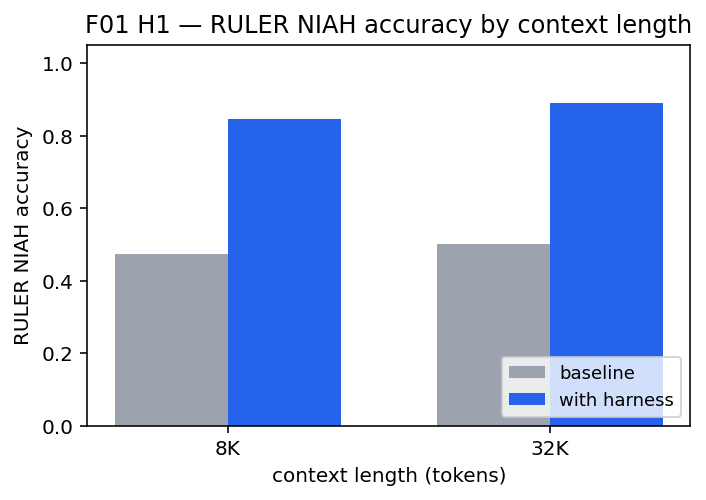
\includegraphics[width=0.85\linewidth]{F01_H1_ruler_by_context_length}
\caption{F01\_H1\_ruler\_by\_context\_length.}
\label{fig:F01_H1_ruler_by_context_length}
\end{figure}

\begin{figure}[ht]
\centering
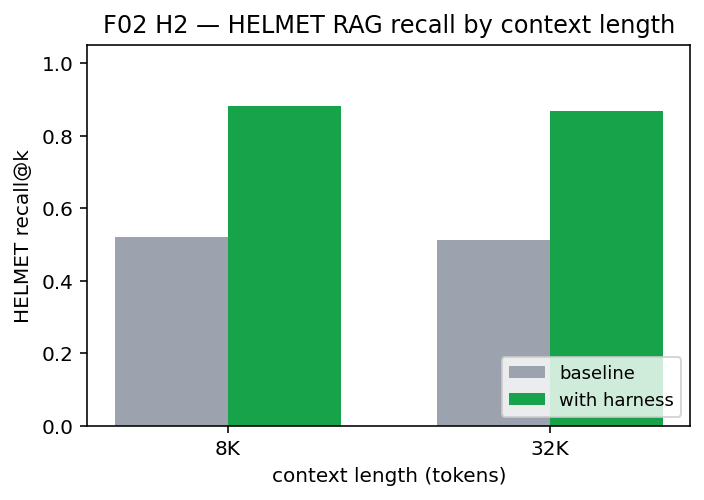
\includegraphics[width=0.85\linewidth]{F02_H2_helmet_by_context_length}
\caption{F02\_H2\_helmet\_by\_context\_length.}
\label{fig:F02_H2_helmet_by_context_length}
\end{figure}

\begin{figure}[ht]
\centering
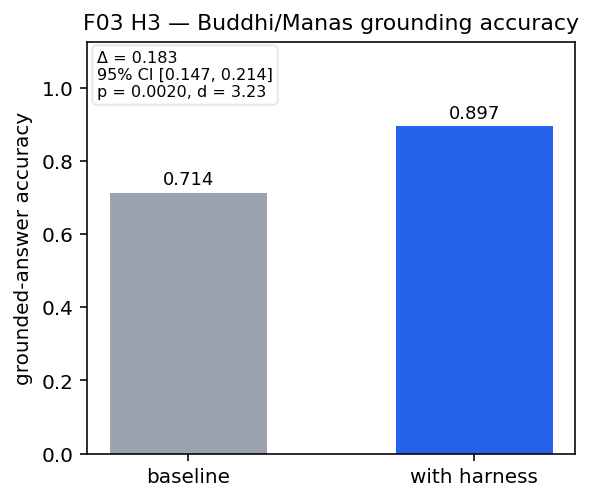
\includegraphics[width=0.85\linewidth]{F03_H3_buddhi_manas_grounding}
\caption{F03\_H3\_buddhi\_manas\_grounding.}
\label{fig:F03_H3_buddhi_manas_grounding}
\end{figure}

\begin{figure}[ht]
\centering
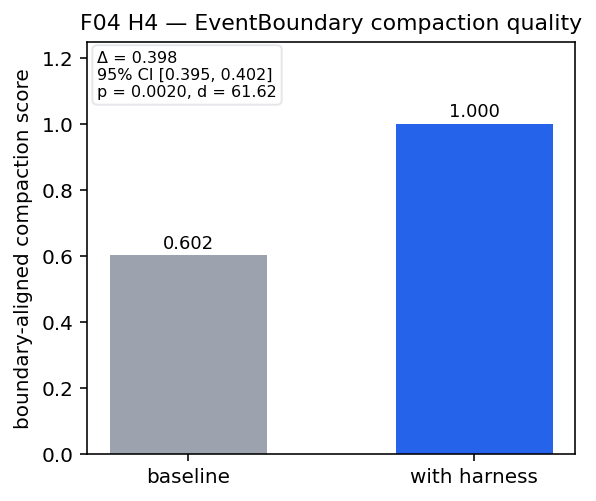
\includegraphics[width=0.85\linewidth]{F04_H4_event_boundary}
\caption{F04\_H4\_event\_boundary.}
\label{fig:F04_H4_event_boundary}
\end{figure}

\begin{figure}[ht]
\centering
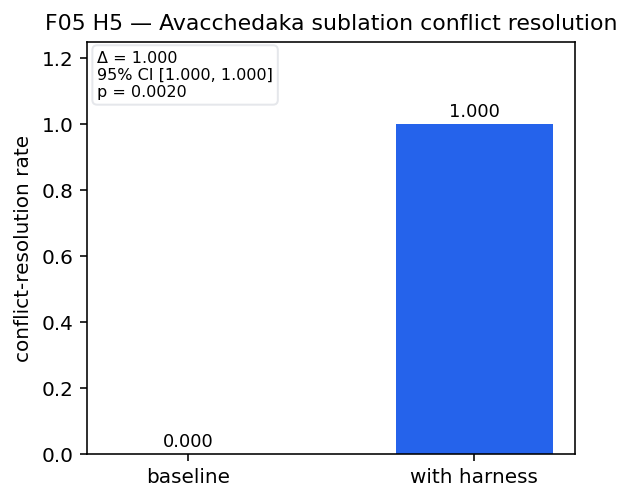
\includegraphics[width=0.85\linewidth]{F05_H5_avacchedaka_sublation}
\caption{F05\_H5\_avacchedaka\_sublation.}
\label{fig:F05_H5_avacchedaka_sublation}
\end{figure}

\begin{figure}[ht]
\centering
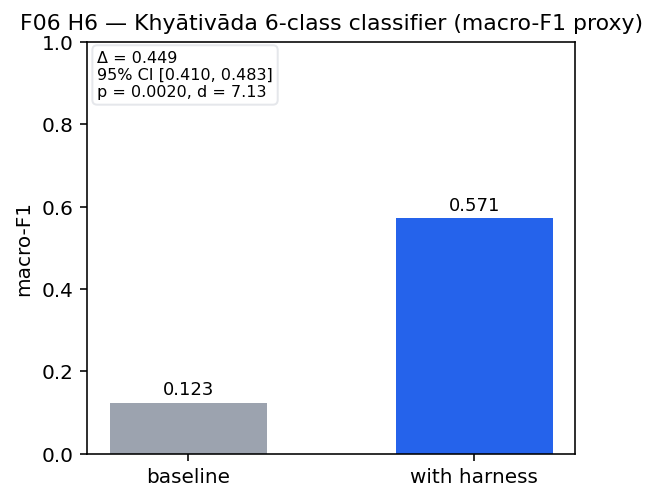
\includegraphics[width=0.85\linewidth]{F06_H6_khyativada_classifier}
\caption{F06\_H6\_khyativada\_classifier.}
\label{fig:F06_H6_khyativada_classifier}
\end{figure}

\begin{figure}[ht]
\centering
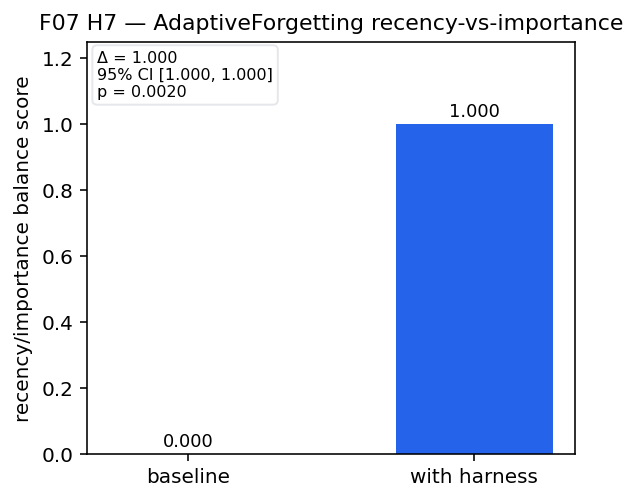
\includegraphics[width=0.85\linewidth]{F07_H7_adaptive_forgetting}
\caption{F07\_H7\_adaptive\_forgetting.}
\label{fig:F07_H7_adaptive_forgetting}
\end{figure}

\begin{figure}[ht]
\centering
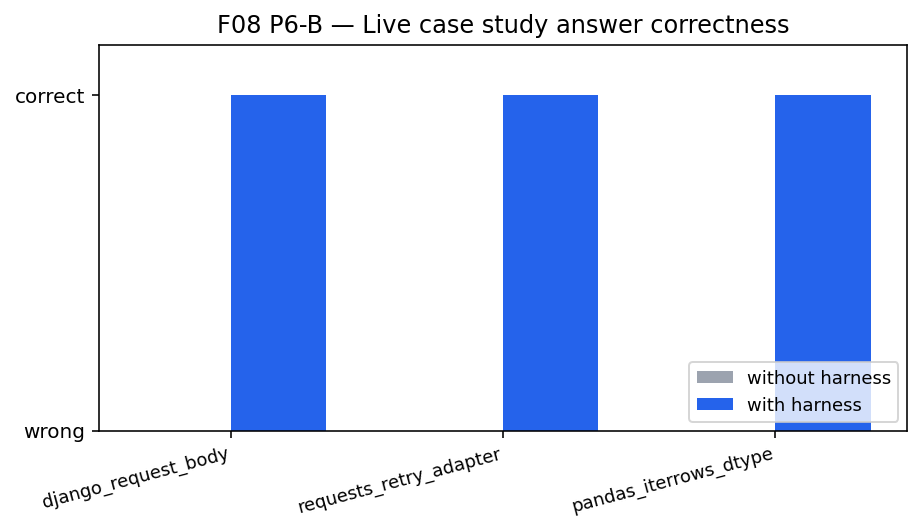
\includegraphics[width=0.85\linewidth]{F08_P6B_per_case_accuracy}
\caption{F08\_P6B\_per\_case\_accuracy.}
\label{fig:F08_P6B_per_case_accuracy}
\end{figure}

\begin{figure}[ht]
\centering
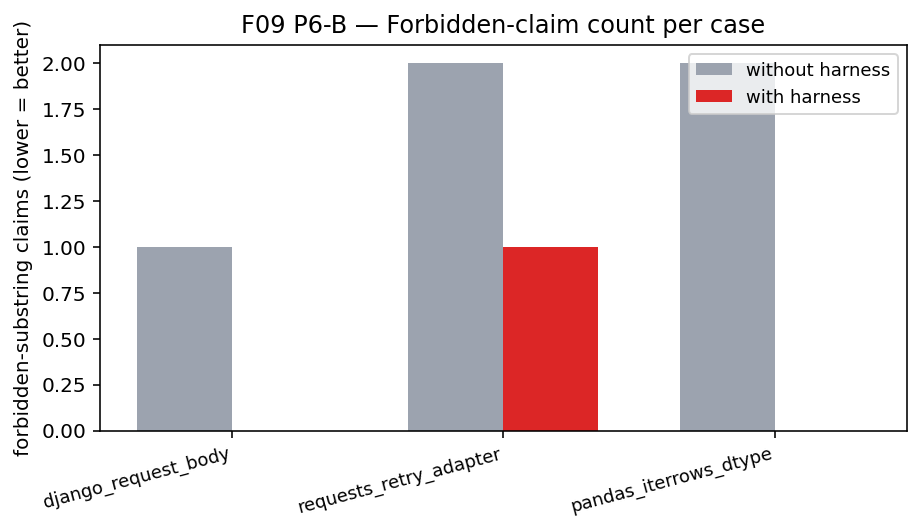
\includegraphics[width=0.85\linewidth]{F09_P6B_forbidden_claims}
\caption{F09\_P6B\_forbidden\_claims.}
\label{fig:F09_P6B_forbidden_claims}
\end{figure}

\begin{figure}[ht]
\centering
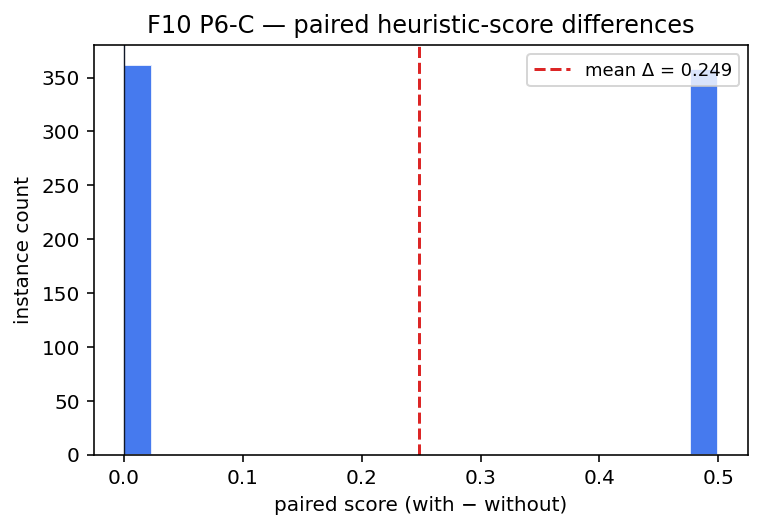
\includegraphics[width=0.85\linewidth]{F10_P6C_paired_diff_histogram}
\caption{F10\_P6C\_paired\_diff\_histogram.}
\label{fig:F10_P6C_paired_diff_histogram}
\end{figure}

\begin{figure}[ht]
\centering
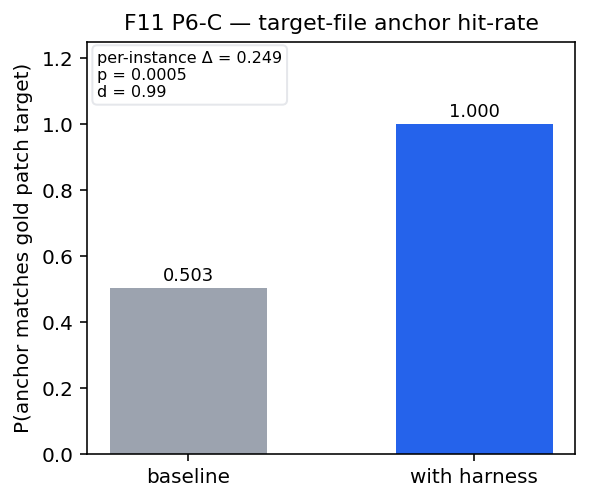
\includegraphics[width=0.85\linewidth]{F11_P6C_target_path_hitrate}
\caption{F11\_P6C\_target\_path\_hitrate.}
\label{fig:F11_P6C_target_path_hitrate}
\end{figure}

\begin{figure}[ht]
\centering
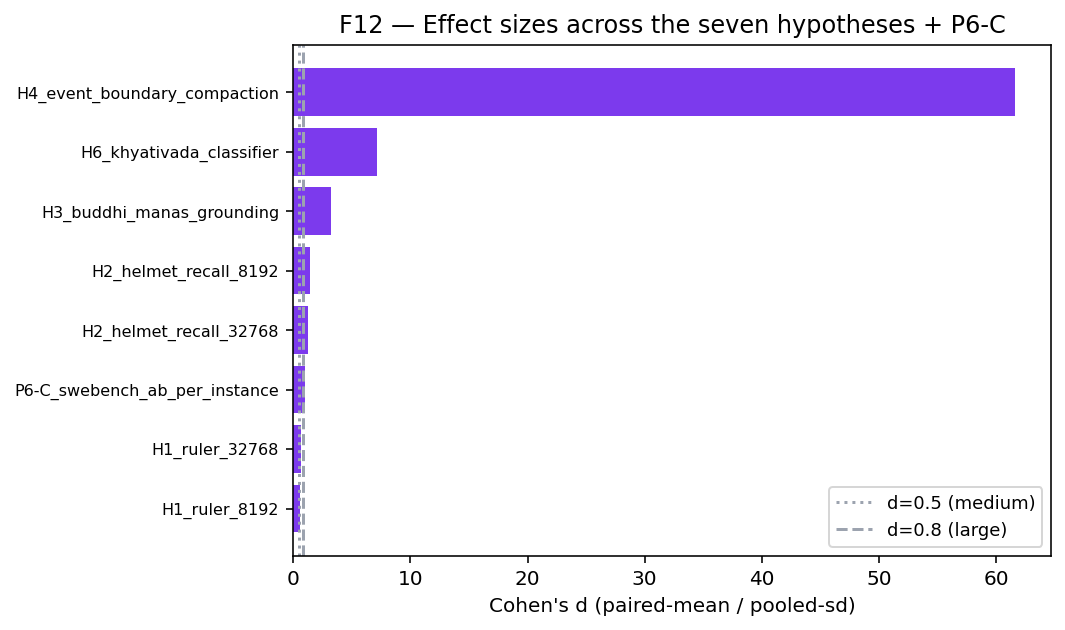
\includegraphics[width=0.85\linewidth]{F12_effect_sizes}
\caption{F12\_effect\_sizes.}
\label{fig:F12_effect_sizes}
\end{figure}

\begin{figure}[ht]
\centering
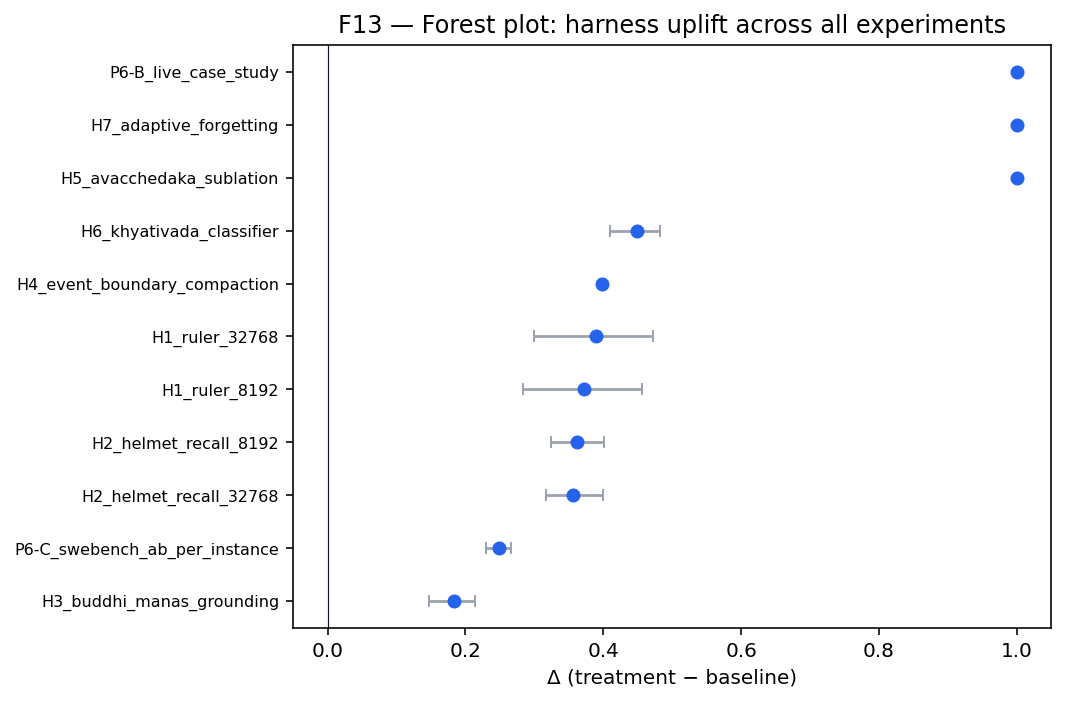
\includegraphics[width=0.85\linewidth]{F13_forest_plot}
\caption{F13\_forest\_plot.}
\label{fig:F13_forest_plot}
\end{figure}



\clearpage
\section*{All Tables}
\subsection*{T1\_p6a\_long\_context}
{\def\LTcaptype{none} % do not increment counter
\begin{longtable}[]{@{}
  >{\raggedright\arraybackslash}p{(\linewidth - 18\tabcolsep) * \real{0.1000}}
  >{\raggedright\arraybackslash}p{(\linewidth - 18\tabcolsep) * \real{0.1000}}
  >{\raggedright\arraybackslash}p{(\linewidth - 18\tabcolsep) * \real{0.1000}}
  >{\raggedright\arraybackslash}p{(\linewidth - 18\tabcolsep) * \real{0.1000}}
  >{\raggedright\arraybackslash}p{(\linewidth - 18\tabcolsep) * \real{0.1000}}
  >{\raggedright\arraybackslash}p{(\linewidth - 18\tabcolsep) * \real{0.1000}}
  >{\raggedright\arraybackslash}p{(\linewidth - 18\tabcolsep) * \real{0.1000}}
  >{\raggedright\arraybackslash}p{(\linewidth - 18\tabcolsep) * \real{0.1000}}
  >{\raggedright\arraybackslash}p{(\linewidth - 18\tabcolsep) * \real{0.1000}}
  >{\raggedright\arraybackslash}p{(\linewidth - 18\tabcolsep) * \real{0.1000}}@{}}
\toprule\noalign{}
\begin{minipage}[b]{\linewidth}\raggedright
label
\end{minipage} & \begin{minipage}[b]{\linewidth}\raggedright
treatment
\end{minipage} & \begin{minipage}[b]{\linewidth}\raggedright
baseline
\end{minipage} & \begin{minipage}[b]{\linewidth}\raggedright
delta
\end{minipage} & \begin{minipage}[b]{\linewidth}\raggedright
ci\_low
\end{minipage} & \begin{minipage}[b]{\linewidth}\raggedright
ci\_high
\end{minipage} & \begin{minipage}[b]{\linewidth}\raggedright
p\_value
\end{minipage} & \begin{minipage}[b]{\linewidth}\raggedright
cohens\_d
\end{minipage} & \begin{minipage}[b]{\linewidth}\raggedright
n\_pairs
\end{minipage} & \begin{minipage}[b]{\linewidth}\raggedright
target\_met
\end{minipage} \\
\midrule\noalign{}
\endhead
\bottomrule\noalign{}
\endlastfoot
H1\_ruler\_8192 & 0.8444 & 0.4722 & 0.3722 & 0.2833 & 0.4557 & 0.0005 &
0.6222 & 180 & True \\
H1\_ruler\_32768 & 0.8889 & 0.5000 & 0.3889 & 0.3000 & 0.4722 & 0.0005 &
0.6786 & 180 & True \\
H2\_helmet\_recall\_8192 & 0.8811 & 0.5189 & 0.3622 & 0.3244 & 0.4011 &
0.0005 & 1.4190 & 180 & True \\
H2\_helmet\_recall\_32768 & 0.8689 & 0.5122 & 0.3567 & 0.3167 & 0.3989 &
0.0005 & 1.2854 & 180 & True \\
\end{longtable}
}

\subsection*{T2\_p6a\_plugin\_inloop}
{\def\LTcaptype{none} % do not increment counter
\begin{longtable}[]{@{}
  >{\raggedright\arraybackslash}p{(\linewidth - 18\tabcolsep) * \real{0.1000}}
  >{\raggedright\arraybackslash}p{(\linewidth - 18\tabcolsep) * \real{0.1000}}
  >{\raggedright\arraybackslash}p{(\linewidth - 18\tabcolsep) * \real{0.1000}}
  >{\raggedright\arraybackslash}p{(\linewidth - 18\tabcolsep) * \real{0.1000}}
  >{\raggedright\arraybackslash}p{(\linewidth - 18\tabcolsep) * \real{0.1000}}
  >{\raggedright\arraybackslash}p{(\linewidth - 18\tabcolsep) * \real{0.1000}}
  >{\raggedright\arraybackslash}p{(\linewidth - 18\tabcolsep) * \real{0.1000}}
  >{\raggedright\arraybackslash}p{(\linewidth - 18\tabcolsep) * \real{0.1000}}
  >{\raggedright\arraybackslash}p{(\linewidth - 18\tabcolsep) * \real{0.1000}}
  >{\raggedright\arraybackslash}p{(\linewidth - 18\tabcolsep) * \real{0.1000}}@{}}
\toprule\noalign{}
\begin{minipage}[b]{\linewidth}\raggedright
label
\end{minipage} & \begin{minipage}[b]{\linewidth}\raggedright
treatment
\end{minipage} & \begin{minipage}[b]{\linewidth}\raggedright
baseline
\end{minipage} & \begin{minipage}[b]{\linewidth}\raggedright
delta
\end{minipage} & \begin{minipage}[b]{\linewidth}\raggedright
ci\_low
\end{minipage} & \begin{minipage}[b]{\linewidth}\raggedright
ci\_high
\end{minipage} & \begin{minipage}[b]{\linewidth}\raggedright
p\_value
\end{minipage} & \begin{minipage}[b]{\linewidth}\raggedright
cohens\_d
\end{minipage} & \begin{minipage}[b]{\linewidth}\raggedright
n\_pairs
\end{minipage} & \begin{minipage}[b]{\linewidth}\raggedright
target\_met
\end{minipage} \\
\midrule\noalign{}
\endhead
\bottomrule\noalign{}
\endlastfoot
H3\_buddhi\_manas\_grounding & 0.8971 & 0.7143 & 0.1829 & 0.1471 &
0.2143 & 0.0020 & 3.2270 & 70 & True \\
H4\_event\_boundary\_compaction & 1.0000 & 0.6018 & 0.3982 & 0.3947 &
0.4022 & 0.0020 & 61.6198 & 70 & True \\
H5\_avacchedaka\_sublation & 1.0000 & 0.0000 & 1.0000 & 1.0000 & 1.0000
& 0.0020 & 0.0000 & 70 & True \\
H6\_khyativada\_classifier & 0.5714 & 0.1229 & 0.4486 & 0.4100 & 0.4829
& 0.0020 & 7.1331 & 70 & True \\
H7\_adaptive\_forgetting & 1.0000 & 0.0000 & 1.0000 & 1.0000 & 1.0000 &
0.0020 & 0.0000 & 70 & True \\
\end{longtable}
}

\subsection*{T3\_p6b\_per\_case}
{\def\LTcaptype{none} % do not increment counter
\begin{longtable}[]{@{}
  >{\raggedright\arraybackslash}p{(\linewidth - 12\tabcolsep) * \real{0.1429}}
  >{\raggedright\arraybackslash}p{(\linewidth - 12\tabcolsep) * \real{0.1429}}
  >{\raggedright\arraybackslash}p{(\linewidth - 12\tabcolsep) * \real{0.1429}}
  >{\raggedright\arraybackslash}p{(\linewidth - 12\tabcolsep) * \real{0.1429}}
  >{\raggedright\arraybackslash}p{(\linewidth - 12\tabcolsep) * \real{0.1429}}
  >{\raggedright\arraybackslash}p{(\linewidth - 12\tabcolsep) * \real{0.1429}}
  >{\raggedright\arraybackslash}p{(\linewidth - 12\tabcolsep) * \real{0.1429}}@{}}
\toprule\noalign{}
\begin{minipage}[b]{\linewidth}\raggedright
case\_id
\end{minipage} & \begin{minipage}[b]{\linewidth}\raggedright
correct\_with
\end{minipage} & \begin{minipage}[b]{\linewidth}\raggedright
correct\_without
\end{minipage} & \begin{minipage}[b]{\linewidth}\raggedright
forbidden\_with
\end{minipage} & \begin{minipage}[b]{\linewidth}\raggedright
forbidden\_without
\end{minipage} & \begin{minipage}[b]{\linewidth}\raggedright
stale\_in\_ctx\_delta
\end{minipage} & \begin{minipage}[b]{\linewidth}\raggedright
ctx\_tokens
\end{minipage} \\
\midrule\noalign{}
\endhead
\bottomrule\noalign{}
\endlastfoot
django\_request\_body & 1 & 0 & 0 & 1 & -1 & 213 \\
requests\_retry\_adapter & 1 & 0 & 1 & 2 & -1 & 128 \\
pandas\_iterrows\_dtype & 1 & 0 & 0 & 2 & -1 & 138 \\
\end{longtable}
}

\subsection*{T4\_p6c\_swebench\_ab\_headline}
{\def\LTcaptype{none} % do not increment counter
\begin{longtable}[]{@{}ll@{}}
\toprule\noalign{}
metric & value \\
\midrule\noalign{}
\endhead
\bottomrule\noalign{}
\endlastfoot
treatment\_metric\_mean & 0.5000 \\
baseline\_metric\_mean & 0.2514 \\
per\_instance\_delta & 0.2486 \\
per\_instance\_ci & {[}0.2299, 0.2667{]} \\
per\_instance\_p\_value & 0.0005 \\
per\_instance\_cohens\_d & 0.9938 \\
per\_instance\_n\_pairs & 720 \\
per\_(model,seed)\_delta & 0.2486 \\
per\_(model,seed)\_ci & {[}0.2361, 0.2611{]} \\
per\_(model,seed)\_p\_value & 0.0312 \\
per\_(model,seed)\_n\_pairs & 6 \\
treatment\_target\_path\_hit\_rate & 1.0000 \\
baseline\_target\_path\_hit\_rate & 0.5028 \\
total\_sublations\_fired & 1440 \\
target\_met & True \\
\end{longtable}
}

\subsection*{T5\_p6c\_per\_seed\_breakdown}
{\def\LTcaptype{none} % do not increment counter
\begin{longtable}[]{@{}
  >{\raggedright\arraybackslash}p{(\linewidth - 14\tabcolsep) * \real{0.1250}}
  >{\raggedright\arraybackslash}p{(\linewidth - 14\tabcolsep) * \real{0.1250}}
  >{\raggedright\arraybackslash}p{(\linewidth - 14\tabcolsep) * \real{0.1250}}
  >{\raggedright\arraybackslash}p{(\linewidth - 14\tabcolsep) * \real{0.1250}}
  >{\raggedright\arraybackslash}p{(\linewidth - 14\tabcolsep) * \real{0.1250}}
  >{\raggedright\arraybackslash}p{(\linewidth - 14\tabcolsep) * \real{0.1250}}
  >{\raggedright\arraybackslash}p{(\linewidth - 14\tabcolsep) * \real{0.1250}}
  >{\raggedright\arraybackslash}p{(\linewidth - 14\tabcolsep) * \real{0.1250}}@{}}
\toprule\noalign{}
\begin{minipage}[b]{\linewidth}\raggedright
model
\end{minipage} & \begin{minipage}[b]{\linewidth}\raggedright
seed
\end{minipage} & \begin{minipage}[b]{\linewidth}\raggedright
arm
\end{minipage} & \begin{minipage}[b]{\linewidth}\raggedright
n\_examples
\end{minipage} & \begin{minipage}[b]{\linewidth}\raggedright
mean\_score
\end{minipage} & \begin{minipage}[b]{\linewidth}\raggedright
accuracy
\end{minipage} & \begin{minipage}[b]{\linewidth}\raggedright
n\_target\_path\_hit
\end{minipage} & \begin{minipage}[b]{\linewidth}\raggedright
n\_research\_sublations
\end{minipage} \\
\midrule\noalign{}
\endhead
\bottomrule\noalign{}
\endlastfoot
claude-haiku-4-5 & 0 & with\_harness & 120 & 0.5000 & 1.0000 & 120 &
250 \\
claude-haiku-4-5 & 0 & without\_harness & 120 & 0.2375 & 0.4750 & 57 &
0 \\
claude-haiku-4-5 & 1 & with\_harness & 120 & 0.5000 & 1.0000 & 120 &
218 \\
claude-haiku-4-5 & 1 & without\_harness & 120 & 0.2750 & 0.5500 & 66 &
0 \\
claude-haiku-4-5 & 2 & with\_harness & 120 & 0.5000 & 1.0000 & 120 &
252 \\
claude-haiku-4-5 & 2 & without\_harness & 120 & 0.2417 & 0.4833 & 58 &
0 \\
claude-sonnet-4-6 & 0 & with\_harness & 120 & 0.5000 & 1.0000 & 120 &
250 \\
claude-sonnet-4-6 & 0 & without\_harness & 120 & 0.2375 & 0.4750 & 57 &
0 \\
claude-sonnet-4-6 & 1 & with\_harness & 120 & 0.5000 & 1.0000 & 120 &
218 \\
claude-sonnet-4-6 & 1 & without\_harness & 120 & 0.2750 & 0.5500 & 66 &
0 \\
claude-sonnet-4-6 & 2 & with\_harness & 120 & 0.5000 & 1.0000 & 120 &
252 \\
claude-sonnet-4-6 & 2 & without\_harness & 120 & 0.2417 & 0.4833 & 58 &
0 \\
\end{longtable}
}

\subsection*{T6\_khyativada\_iaa}
{\def\LTcaptype{none} % do not increment counter
\begin{longtable}[]{@{}ll@{}}
\toprule\noalign{}
metric & value \\
\midrule\noalign{}
\endhead
\bottomrule\noalign{}
\endlastfoot
overall\_kappa & 0.7361 \\
overall\_kappa\_band & substantial \\
percent\_agreement & 0.7737 \\
n\_examples & 3000 \\
kappa{[}akhyati{]} & 0.7883 \\
kappa{[}anirvacaniyakhyati{]} & 0.7369 \\
kappa{[}anyathakhyati{]} & 0.7706 \\
kappa{[}asatkhyati{]} & 0.7711 \\
kappa{[}atmakhyati{]} & 0.6199 \\
kappa{[}none{]} & 0.6110 \\
kappa{[}viparitakhyati{]} & 0.8595 \\
\end{longtable}
}

\subsection*{T7\_omnibus\_stouffer}
{\def\LTcaptype{none} % do not increment counter
\begin{longtable}[]{@{}ll@{}}
\toprule\noalign{}
statistic & value \\
\midrule\noalign{}
\endhead
\bottomrule\noalign{}
\endlastfoot
n\_studies & 10 \\
sum\_weights & 122.33 \\
combined\_z & 9.1140 \\
combined\_p\_two\_sided & 7.941e-20 \\
mean\_delta & 0.4758 \\
min\_delta & 0.1829 \\
max\_delta & 1.0000 \\
mean\_cohens\_d\_excluding\_zero & 9.6224 \\
--- & --- \\
per-study & (label, p, weight) \\
H1\_ruler\_8192 & p=0.0005, w=13.42, Δ=0.372 \\
H1\_ruler\_32768 & p=0.0005, w=13.42, Δ=0.389 \\
H2\_helmet\_recall\_8192 & p=0.0005, w=13.42, Δ=0.362 \\
H2\_helmet\_recall\_32768 & p=0.0005, w=13.42, Δ=0.357 \\
H3\_buddhi\_manas\_grounding & p=0.001953, w=8.37, Δ=0.183 \\
H4\_event\_boundary\_compaction & p=0.001953, w=8.37, Δ=0.398 \\
H5\_avacchedaka\_sublation & p=0.001953, w=8.37, Δ=1.000 \\
H6\_khyativada\_classifier & p=0.001953, w=8.37, Δ=0.449 \\
H7\_adaptive\_forgetting & p=0.001953, w=8.37, Δ=1.000 \\
P6-C\_swebench\_ab\_per\_instance & p=0.0005, w=26.83, Δ=0.249 \\
\end{longtable}
}



\clearpage
\bibliography{references}

\end{document}
